\documentclass[12pt,a4paper]{article}
\usepackage{../.tex/mcs-notes}
\usepackage{todonotes}
\usepackage{multicol}
\usepackage{inkscape}
\usepackage[all]{xy}
\CompileMatrices

\settitle
{Геометрия и топология.}
{Евгений Анатольевич Фоминых}
{geometry-and-topology/main.pdf}
\date{}

\newcommand{\Id}{\ensuremath{\mathrm{Id}}\xspace}
\newcommand{\Ker}{\ensuremath{\mathrm{Ker}}\xspace}
\newcommand{\Img}{\ensuremath{\mathrm{Im}}\xspace}
\newcommand{\diam}{\ensuremath{\mathrm{diam}}\xspace}
\newcommand{\Int}{\ensuremath{\mathrm{Int}}\xspace}
\newcommand{\Ext}{\ensuremath{\mathrm{Ext}}\xspace}
\newcommand{\Cl}{\ensuremath{\mathrm{Cl}}\xspace}
\newcommand{\Fr}{\ensuremath{\mathrm{Fr}}\xspace}
\newcommand{\SCl}{\ensuremath{\mathrm{SCl}}\xspace}
\newcommand{\Lin}{\ensuremath{\mathrm{Lin}}\xspace}
\newcommand{\Homeo}{\ensuremath{\mathrm{Homeo}}\xspace}
\newcommand{\Aff}{\ensuremath{\mathrm{Aff}}\xspace}
\newcommand{\Iso}{\ensuremath{\mathrm{Iso}}\xspace}
\renewcommand{\Pr}{\ensuremath{\mathrm{Pr}}\xspace}
\newcommand{\conv}{\ensuremath{\mathrm{conv}}\xspace}
\newcommand{\RelInt}{\ensuremath{\mathrm{RelInt}}\xspace}
\DeclareMathOperator*{\bigtimes}{\text{\raisebox{-6pt}{\scalebox{3}{$\times$}}}}
\newcommand{\FAC}{\ensuremath{\mathrm{FAC}}\xspace}
\newcommand{\SAC}{\ensuremath{\mathrm{SAC}}\xspace}
\newcommand{\T}{\ensuremath{\mathrm{T}}\xspace}
\newcommand{\ex}{\ensuremath{\mathrm{ex}}\xspace}
\newcommand{\ind}{\ensuremath{\mathrm{ind}}\xspace}

\begin{document}
    \maketitle

    \listoftodos[TODOs]

    \tableofcontents

    \vspace{2em}

    Литература:
    \begin{itemize}
        \item Виро О.Я., Иванов О.А., Нецветаев Н.Ю., Харламов В.М., ``Элементарная топология'', М.:МЦНМО, 2012.
        \item Коснёвски Чес, ``Начальный курс алгебраической топологии'', М.:Мир, 1983.
        \item Ю.Г. Борисович, Н.М. Близняков, Я.А. Израилевич, Т.Н. Фоменко, ``Введение в топологию'', М.:Наука. Физматлит, 1995.
        \item James Munkres, ``Topology''.
        \item Agusti Reventos Tarrida, ``Affine maps, Euclidean motions and quadrics''.
        \item Винберг, ``Курс алгебры''.
        \item Хатчер, ``Алгебраическая топология''. 
    \end{itemize}

    \section{Метрические и топологические пространства. Базовые понятия.}
    
    \subsection{Метрические пространства.}

    \begin{definition}
        Функция $d: X \times X \to \RR_+$ называется \emph{метрикой} (или \emph{расстоянием}) в множестве $X$, если:
        \begin{itemize}
            \item $d(x, y) = 0 \Leftrightarrow x = y$;
            \item $d(x, y) = d(y, x)$;
            \item $d(x, z) \leqslant d(x, y) + d(y, z)$ (``неравенство треугольника'').
        \end{itemize}
        Пара $(X, d)$, где $d$ --- метрика в $X$, называется \emph{метрическим пространством}.
    \end{definition}

    \begin{example}
        Пусть $X$ --- произвольное множество. Тогда метрика
        \[
            d(x, y) := 
                \begin{cases}
                    1& \text{если $x \neq y$}\\
                    0& \text{если $x = y$}
                \end{cases}
        \]
        называется \emph{дискретной} метрикой на множестве $X$.
    \end{example}

    \begin{example}\ 
        \begin{itemize}
            \item $X := \RR$, тогда $d(x, y) := |x-y|$ --- метрика.
            \item $X := \RR^n$, $x = (x_1, \dots, x_n)$, $y = (y_1, \dots, y_n)$. Тогда
                \[d(x, y) := \sqrt{(x_1 - y_1)^2 + \dots + (x_n + y_n)^2}\]
                называется \emph{евклидовой} метрикой.
            \item $X := \RR^n$, $d(x, y) := \max_{i = 1}^n |x_i - y_i|$
            \item $X := \RR^n$, $d(x, y) := \sum_{i = 1}^n |x_i - y_i|$
            \item $X := C[0; 1]$, $d(x(t), y(t)) = \max_{t \in [0; 1]} |x(t) - y(t)|$. $(X, d)$ называют \emph{пространством непрерывных функций}.
        \end{itemize}
    \end{example}

    \begin{definition}
        Пусть $(X, d)$ --- метрическое пространство. Сужение функции $d$ на $Y \times Y$ является метрикой в $Y$. Метрическое пространство $(Y, d|_{Y\times Y})$ называется \emph{подпространством} пространства $(X, d)$.
    \end{definition}

    \begin{theorem}\label{generalised_metric_spaces_multiplication_theorem}
        Пусть дана $g: \RR_+ \times \RR_+ \to \RR_+$, что
        \begin{itemize}
            \item $\forall x, y \in \RR_+\quad g(x, y) = 0 \leftrightarrow x = y = 0$;
            \item $\forall x, y, d \in \RR_+\quad g(x + d, y) \geqslant g(x, y) \wedge g(x, y + d) \geqslant g(x, y)$;
            \item $\forall x_1, y_1, x_2, y_2 \in \RR_+ \quad g(x_1 + x_2, y_1 + y_2) \leqslant g(x_1, y_1) + g(x_2, y_2)$.
        \end{itemize}
        Тогда для любых метрических пространств $(X, d_X)$ и $(Y, d_Y)$ функция
        \[d_{X \times Y}((x_1, y_1), (x_2, y_2)) := g(d_X(x_1, x_2), d_Y(y_1, y_2))\]
        будет метрикой на $X \times Y$.
    \end{theorem}

    \begin{proof}
        Проверим, что $d_{X \times Y}$ --- метрика.
        \begin{itemize}
            \item $\forall x_1, x_2 \in X, y_1, y_2 \in Y$
                \begin{align*}
                    d_{X \times Y}((x_1, y_1), (x_2, y_2)) = 0\quad
                    &\longleftrightarrow\quad g(d_X(x_1, x_2), d_Y(y_1, y_2)) = 0\\
                    &\longleftrightarrow\quad d_X(x_1, x_2) = 0 \wedge d_Y(y_1, y_2) = 0\\
                    &\longleftrightarrow\quad x_1 = x_2 \wedge y_1 = y_2
                \end{align*}
            \item $\forall x_1, x_2 \in X, y_1, y_2 \in Y$
                \begin{multline*}
                    d_{X \times Y}((x_1, y_1), (x_2, y_2))\\
                    = g(d_X(x_1, x_2), d_Y(y_1, y_2)) = g(d_X(x_2, x_1), d_Y(y_2, y_1))\\
                    = d_{X \times Y}((x_2, y_2), (x_1, y_1))
                \end{multline*}
            \item $\forall x_1, x_2, x_3 \in X, y_1, y_2, y_3 \in Y$
                \begin{multline*}
                    d_{X \times Y}((x_1, y_1), (x_3, y_3))\\
                    = g(d_X(x_1, x_3), d_Y(y_1, y_3))\\
                    \leqslant g(d_X(x_1, x_2) + d_X(x_2, x_3), d_Y(y_1, y_2) + d_Y(y_2, y_3))\\
                    \leqslant g(d_X(x_1, x_2), d_Y(y_1, y_2)) + g(d_X(x_2, x_3), d_Y(y_2, y_3))\\
                    = d_{X \times Y}((x_1, y_1), (x_2, y_2)) + d_{X \times Y}((x_2, y_2), (x_3, y_3))
                \end{multline*}
        \end{itemize}
    \end{proof}

    \begin{corollary}
        Для любых метрических пространств $(X, d_X)$ и $(Y, d_Y)$ пара $(X \times Y, d_{X \times Y})$, где
        \[d_{X \times Y} := \sqrt{d_X(x_1, x_2)^2 + d_Y(y_1, y_2)^2}\]
        есть метрическое пространство.
    \end{corollary}

    \begin{proof}
        Необходимо лишь проверить, что $g(x, y) := \sqrt{x^2 + y^2}$ удовлетворяет условиям теоремы.
        \begin{itemize}
            \item $\forall x, y \in \RR_+\quad \sqrt{x^2 + y^2} \leftrightarrow x^2 + y^2 = 0 \leftrightarrow x = 0 = y$.
            \item $\forall x, y, d \in \RR_+\quad x+d \geqslant x \Rightarrow (x+d)^2 \geqslant x^2 \Rightarrow (x+d)^2 + y^2 \geqslant x^2 + y^2 \Rightarrow \sqrt{(x+d)^2 + y^2} \geqslant \sqrt{x^2 + y^2}$; для $y$ аналогично.
            \item $\forall x_1, y_1, x_2, y_2 \in \RR_+$ по неравенству Коши-Буняковского-Шварца
            \begin{gather*}
                (x_1y_2 - x_2y_1)^2 \geqslant 0\\
                x_1^2y_2^2 + x_2^2y_1^2 \geqslant 2x_1x_2y_1y_2\\
                (x_1^2 + y_1^2)(x_2^2 + y_2^2) \geqslant (x_1x_2 + y_1y_2)^2\\
                (x_1^2 + y_1^2) + 2\sqrt{(x_1^2 + y_1^2)(x_2^2 + y_2^2)} + (x_2^2 + y_2^2) \geqslant (x_1^2 + y_1^2) + 2(x_1x_2 + y_1y_2) + (x_2^2 + y_2^2)\\
                \left(\sqrt{x_1^2 + y_1^2} + \sqrt{x_2^2 + y_2^2}\right)^2 \geqslant (x_1 + x_2)^2 + (y_1 + y_2)^2\\
                \sqrt{x_1^2 + y_1^2} + \sqrt{x_2^2 + y_2^2} \geqslant \sqrt{(x_1 + x_2)^2 + (y_1 + y_2)^2}
            \end{gather*}
        \end{itemize}
    \end{proof}

    \begin{remark}
        Если $g$ ассоциативна (например, $g(x, y) := \sqrt{x^2 + y^2}$; она заодно коммутативна), то аналогично можно определить метрику на $X_1 \times X_2 \times \dots \times X_n = (X_1 \times (X_2 \times (\dots \times X_n)\dots))$.

        Таким образом евклидова метрика есть метрика, так как её можно получить, применяя $g(x, y) := \sqrt{x^2 + y^2}$ к пространствам $(X_i, d_i) = (\RR, d_{\RR})$ (где $d_{\RR}(x, y) = |x-y|$).
    \end{remark}

    \begin{definition}
        Пусть 
        Для $g(x, y) := \sqrt{x^2 + y^2}$ из последней теоремы пространство $(X \times Y, d_{X \times Y})$ называется \emph{(декартовым) произведением} метрических пространств $(X, d_X)$ и $(Y, d_Y)$. Аналогично определяется произведение конечного числа пространств.
    \end{definition}

    \begin{remark}
        На роль $g(x, y)$ подходят следующие функции:
        \begin{itemize}
            \item $(x^\alpha + y^\alpha)^{1/\alpha}$ для всех $\alpha \geqslant 1$;
            \item $\max(x, y)$.
        \end{itemize}
        А следующие функции уже не подходят:
        \begin{itemize}
            \item $(x^\alpha + y^\alpha)^{1/\alpha}$ для всех $\alpha < 1$ (даже для отрицательных);
            \item $\min(x, y)$;
            \item $x \cdot y$ и $x / y$.
        \end{itemize}
    \end{remark}

    \begin{definition}
        Пусть $(X, d)$ --- метрическое пространство, $a \in X$, $r \in \RR$, $r > 0$. Тогда:
        \begin{itemize}
            \item $B_r(a) := \{x \in X \mid d(a, x) < r\}$ --- \emph{(открытый) шар пространства $(X, d)$ с центром в точке $a$ и радиусом $r$};
            \item $\overline{B}_r(a) = D_r(a) := \{x \in X \mid d(a, x) \leqslant r\}$ --- \emph{замкнутой шар пространства $(X, d)$ с центром в точке $a$ и радиусом $r$};
            \item $S_r(a) := \{x \in X \mid d(a, x) = r\}$ --- \emph{сфера пространства $(X, d)$ с центром в точке $a$ и радиусом $r$}.
        \end{itemize}
    \end{definition}

    \begin{definition}
        Пусть $(X, d)$ --- метрическое пространство, $A \subseteq X$. Множество $A$ называется \emph{открытым} в метрическом пространстве, если
        \[\forall a \in A\ \exists r > 0: B_r(a) \subseteq A\]
    \end{definition}

    \begin{theorem}В любом метрическом пространстве $(X, d)$
        \begin{enumerate}
            \item $\varnothing$ и $X$ открыты;
            \item для всяких $a \in X$ и $r > 0$ открытый шар $B_r(a)$ открыт; 
            \item объединение любого семейства открытых множеств открыто;
            \item пересечение конечного семейства открытых множеств открыто.
        \end{enumerate}
    \end{theorem}

    \begin{proof}\ 
        \begin{enumerate}
            \item Очевидно.
            \item Для всякого $x \in B_r(a)$ верно, что $B_{r-d(x, a)}(x) \subseteq B_r(a)$, откуда утверждение очевидно следует.
            \item Пусть дано семейство открытых множеств $\Sigma$. Пусть также $I = \bigcup \Sigma$. Для любого $x \in I$ верно, что существует $J \in \Sigma$, что $x \in J$, а значит есть $r > 0$, что $B_r(x) \subseteq J \subseteq I$, т.е. $x$ --- внутренняя точка $I$. Таким образом $I$ открыто.
            \item Пусть $I = \bigcap_{i = 1}^n I_i$. Тогда для любого $x \in I$ верно, что существуют $r_1, \dots, r_n > 0$, что $B_{r_i}(x) \subseteq I_n$, значит $B_{\min r_i} \subseteq I$, значит $x$ --- внутренняя точка $I$. Таким образом $I$ открыто.
        \end{enumerate}
    \end{proof}

    \subsection{Топологические пространства.}

    \begin{definition}
        Пусть $X$ --- некоторое множество. Рассмотрим набор $\Omega$ его подмножеств, для которого:
        \begin{enumerate}
            \item $\varnothing, X \in \Omega$;
            \item объединение любого семейства множеств из $\Omega$ лежит в $\Omega$;
            \item пересечение любого конечного семейства множеств, принадлежащих $\Omega$, также принадлежит $\Omega$.
        \end{enumerate}
        В таком случае:
        \begin{itemize}
            \item $\Omega$ --- \emph{топологическая структура} или просто \emph{топология} в множестве $X$;
            \item множество $X$ с выделенной топологической структурой $\Omega$ (т.е.пара $(X, \Omega)$) называется \emph{топологическим пространством};
            \item элементы множества $\Omega$ называются \emph{открытыми множествами} пространства $(X, \Omega)$.
        \end{itemize}
    \end{definition}

    \begin{example}\ 
        \begin{itemize}
            \item Если $\Omega$ --- множество открытых множеств в метрическом пространстве $(X, d)$, то $(X, \Omega)$ --- топологическое пространство. Таким образом любое метрическое пространство можно отождествлять с соответствующим топологическим пространством.
            \item Топология, индуцированная евклидовой метрикой в $\RR^n$, называется \emph{стандартной}.
            \item $\Omega := 2^X$ --- \emph{дискретная} топология на произвольном множестве $X$. Именно она порождается дискретной метрикой на $X$.
            \item $\Omega := \{\varnothing, X\}$ --- \emph{антидискретная} топология на произвольном множестве $X$.
            \item $X := \RR$, $\Omega := \{(a; +\infty) : a \in \RR\} \cup \{\RR\} \cup \{\varnothing\}$. Такая топология называется \emph{стрелкой}.
            \item $\Omega = \{\varnothing\} \cup \{A \in X: |X\setminus A| \in \NN\}$ --- топология \emph{конечных дополнений} на произвольном множестве $X$.
        \end{itemize}
    \end{example}

    \begin{definition}
        Множество $F \subseteq X$ \emph{замкнуто} в топологическом пространстве $(X, \Sigma)$, если его дополнение $X \setminus F$ открыто (т.е. если $X \setminus F \in \Sigma$).
    \end{definition}

    \begin{theorem}
        В любом топологическом пространстве $X$
        \begin{itemize}
            \item $\varnothing$ и $X$ --- замкнуты;
            \item объединение конечного набора замкнутых множеств замкнуто;
            \item пересечение любого набора замкнутых множеств замкнуто.
        \end{itemize}
    \end{theorem}

    \begin{theorem}
        Пусть $U$ --- открыто, а $V$ --- замкнуто в $(X, \Omega)$. Тогда:
        \begin{multicols}{2}
            \begin{itemize}
                \item $U \setminus V$ открыто;
                \item $V \setminus U$ замкнуто.
            \end{itemize}
        \end{multicols}
    \end{theorem}

    \subsection{Внутренность и замыкание множества. Разные виды точек.}

    \begin{definition}
        Пусть $(X, \Omega)$ --- топологическое пространство и $A \subseteq X$. Тогда \emph{внутренностью} множества $A$ называется
        объединение всех открытых подмножеств $A$:
        \[\Int(A) := \bigcup_{\substack{U \in \Omega\\U \subseteq A}} U\]
    \end{definition}

    \begin{theorem}\ 
        \begin{multicols}{2}
            \begin{itemize}
                \item $\Int(A)$ --- открытое множество.
                \item $\Int(A) \subseteq A$.
                \item $B\text{ --- открыто} \wedge B \subseteq A \Rightarrow B \subseteq \Int(A)$.
                \item $A = \Int(A) \Leftrightarrow A \text{ --- открыто}$.
                \item $\Int(\Int(A)) = \Int(A)$.
                \item $A \subseteq B \Rightarrow \Int(A) \subseteq \Int(B)$.
                \item $\Int(\bigcap_{k=1}^n A_k) = \bigcap_{k=1}^n \Int(A_k)$.
                \item $\Int(\bigcup_{A \in \Sigma} A) \supseteq \bigcup_{A \in \Sigma} \Int(A)$.
            \end{itemize}
        \end{multicols}
    \end{theorem}

    \begin{definition}
        \emph{Окрестность} точки $a$ в топологическом пространстве $X$ --- открытое множество в $X$, содержащее $a$.

        Точка $a$ топологического пространства $X$ называется \emph{внутренней точкой} множества $A \subseteq X$, если $A$ содержит как подмножество некоторую окрестность $a$.
    \end{definition}

    \begin{theorem}\ 
        \begin{itemize}
            \item Множество открыто тогда и только тогда, когда все его точки внутренние.
            \item Внутренность множества есть множество всех его внутренних точек.
        \end{itemize}
    \end{theorem}

    \begin{proof}\ 
        \begin{itemize}
            \item
                \begin{itemize}
                    \item[($\Rightarrow$)] Пусть $A$ открыто, а $a \in A$. Тогда $A$ --- та самая окрестность $a$, которая является подмножеством $A$, поэтому $a$ --- внутренняя точка $A$.
                    \item[($\Leftarrow$)] Пусть каждая точка $A$ внутренняя. Тогда для каждого $a \in A$ определим окрестность $I_a$, лежащую в $A$ как подмножество (такая есть по определению). Тем самым $A = \bigcup_{a \in A} I_a$, т.е. $A$ есть объединение открытых множеств, следовательно открытое множество.
                \end{itemize}
            \item
                \begin{itemize}
                    \item[($\subseteq$)] Пусть $a \in \Int(A)$. Вспомним, что $\Int(A)$ --- открытое подмножество $A$. Следовательно, $a$ --- внутренняя точка $A$.
                    \item[($\supseteq$)] Пусть $a$ --- внутренняя точка $A$. Следовательно есть открытое $I$, что $a \in I \subseteq A$, следовательно $I \subseteq \Int(A)$, а значит $a \in \Int(A)$.
                \end{itemize}
        \end{itemize}
    \end{proof}

    \begin{definition}
        Пусть $(X, \Omega)$ --- топологическое пространство, а $A \subseteq X$. \emph{Замыканием} множества $A$ называется пересечение всех замкнутых пространств, содержащих $A$ как подмножество:
        \[\Cl(A) := \bigcap_{\substack{X \setminus V \in \Omega\\V\supseteq A}} V\]
    \end{definition}

    \begin{theorem}\ 
        \begin{multicols}{2}
            \begin{itemize}
                \item $\Cl(A)$ --- замкнутое множество.
                \item $\Cl(A) \supseteq A$.
                \item $B\text{ --- замкнуто} \wedge B \supseteq A \Rightarrow B \supseteq \Cl(A)$.
                \item $A = \Cl(A) \Leftrightarrow A \text{ --- замкнуто}$.
                \item $\Cl(\Cl(A)) = \Cl(A)$.
                \item $A \subseteq B \Rightarrow \Cl(A) \subseteq \Cl(B)$.
                \item $\Cl(\bigcup_{k=1}^n A_k) = \bigcup_{k=1}^n \Cl(A_k)$.
                \item $\Cl(\bigcap_{A \in \Sigma} A) \subseteq \bigcap_{A \in \Sigma} \Cl(A)$.
                \item $\Cl(A) \sqcup \Int(X \setminus A) = X$.
            \end{itemize}
        \end{multicols}
    \end{theorem}

    \begin{definition}
        Пусть $X$ --- топологическое пространство, $A \subseteq X$ и $b \in X$. Точка $b$ называется \emph{точкой прикосновения} множества $A$, если всякая её окрестность пересекается с $A$.
    \end{definition}

    \begin{theorem}\ 
        \begin{itemize}
            \item Множество замкнуто тогда и только тогда, когда оно является множеством своих точек прикосновения.
            \item Замыкание множества есть множество всех его точек прикосновения.
        \end{itemize}
    \end{theorem}

    \begin{definition}
        Пусть $X$ --- топологическое пространство, $A \subseteq X$ и $a \in X$.

        \emph{Граница} множества $A$ --- разность замыкания и внутренности $A$: $\Fr(A) := \Cl(A) \setminus \Int(A)$.

        Точка $a$ --- \emph{граничная точка} множества $A$, если всякая её окрестность пересекается с $A$ и с $X \setminus A$.
    \end{definition}

    \begin{theorem}
        Граница множества совпадает с множеством его граничных точек.
    \end{theorem}

    \begin{theorem}\ 
        \begin{multicols}{2}
            \begin{itemize}
                \item $\Fr(A)$ замкнуто.
                \item $\Fr(A) = \Fr(X \setminus A)$.
                \item $A\text{ замкнуто} \Leftrightarrow A \supseteq \Fr(A)$.
                \item $A\text{ открыто} \Leftrightarrow A \cap \Fr(A) = \varnothing$.
            \end{itemize}
        \end{multicols}
    \end{theorem}

    \begin{definition}
        Пусть $X$ --- топологическое пространство, $A \subseteq X$ и $a \in X$.

        $a$ --- \emph{предельная точка} $A$, если в любой окрестности $a$ есть точка $A \setminus \{a\}$.

        $a$ --- \emph{изолированная точка} $A$, если $a \in A$ и есть окрестность $a$ без точка $A \setminus \{a\}$.
    \end{definition}

    \begin{theorem}\ 
        \begin{itemize}
            \item $b\text{ --- предельная} \Rightarrow b\text{ --- точка прикосновения}$.
            \item $\Cl(A) = \{\text{внутренние точки $A$}\} \sqcup \{\text{граничные точки $A$}\}$.
            \item $\Cl(A) = \{\text{предельные точки $A$}\} \sqcup \{\text{изолированные точки $A$}\}$.
        \end{itemize}
    \end{theorem}

    \subsection{Сравнение топологий.}

    \begin{definition}
        Пусть $\Omega_1$ и $\Omega_2$ --- топологии на $X$. Тогда если $\Omega_1 \subseteq \Omega_2$, то говорят, что $\Omega_1$ \emph{слабее (грубее)} $\Omega_2$, а $\Omega_2$ \emph{сильнее (тоньше)} $\Omega_1$.
    \end{definition}

    \begin{example}
        Из всех топологий на $X$ антидискретная --- самая грубая, а дискретная --- самая тонкая.
    \end{example}

    \begin{theorem}\label{metric_generated_topologies_comparation_theorem}
        Топология метрики $d_1$ грубее топологии метрики $d_2$ тогда и только тогда, когда в любом шаре метрики $d_1$ содержится шар метрики $d_2$ с тем же центром.
    \end{theorem}

    \begin{proof}
        \begin{itemize}
            \item[($\Rightarrow$)] Пусть топология метрики $d_1$ грубее топологии метрики $d_2$. Тогда любой шар $B_r^{d_1}(a)$ открыт в $d_2$, следовательно по определению открытости есть шар $B_q^{d_2}(a) \subseteq B_r^{d_1}(a)$.
            \item[($\Leftarrow$)] Пусть в любом шаре метрики $d_1$ содержится шар метрики $d_2$ с тем же центром. Возьмём любое открытое в $d_1$ множество $U$. Тогда для всякой точки $a \in U$ есть шар $B_r^{d_1}(a) \subseteq U$. При этом есть шар $B_q^{d_2}(a) \subseteq B_r^{d_1}(a)$, таким образом $a$ --- внутренняя точка $U$ в $d_2$. Следовательно $U$ открыто в $d_2$.
        \end{itemize}
    \end{proof}

    \begin{corollary}
        Если $d_1$ и $d_2$ --- метрики на $X$ и $d_1 \leqslant d_2$, то топология $d_1$ грубее топологии $d_2$. 
    \end{corollary}

    \begin{definition}
        Две метрики на одном множестве называются \emph{эквивалентными}, если они порождают одну топологию.
    \end{definition}

    \begin{lemma}
        Пусть $(X, d)$ --- метрическое пространство. Тогда для всякого $C > 0$ функция $C \cdot d$ --- метрика на $X$, эквивалентная $d$. 
    \end{lemma}

    \begin{corollary}
        Если для метрик $d_1$ и $d_2$ на $X$ есть такое $C > 0$, что $d_1 \leqslant C d_2$, то $d_1$ грубее $d_2$.
    \end{corollary}

    \begin{definition}
        Метрики $d_1$ и $d_2$ на одном множестве называются \emph{липшицево эквивалентными}, если существуют $c, C > 0$, что $c \cdot d_1 \leqslant d_2 \leqslant C \cdot d_1$.
    \end{definition}

    \begin{theorem}
        Липшицево эквивалентные метрики просто эквивалентны.
    \end{theorem}

    \begin{definition}
        Топологическое пространство \emph{метризуемо}, если есть метрика, её порождающая.
    \end{definition}

    \subsection{База и предбаза топологии.}

    \begin{definition}
        \emph{База} топологии $\Omega$ --- такое семейство $\Sigma$ открытых множеств, что всякое открытое $U$ представимо в виде объединения множеств из $\Sigma$.
        \[\Sigma \subseteq \Omega\text{ --- база} \Longleftrightarrow \forall U \in \Omega\; \exists \Lambda \subseteq \Sigma:\quad U = \bigcup_{W \in \Lambda} W\]
    \end{definition}

    \begin{definition}
        Множество $\Gamma$ подмножеств множества $X$ называется его \emph{покрытием}, если $X := \bigcup_{A \in \Gamma} A$. Часто покрытие записывают в виде $\Gamma = \{A_i\}_{i \in I}$.
    \end{definition}

    \begin{theorem}[второе определение базы]
        Пусть $(X, \Omega)$ --- топологическое пространство и $\Sigma \subseteq \Omega$. Тогда $\Sigma$ --- база топологии $\Omega$ тогда и только тогда, когда для любой точки $a$ любого открытого множества $U$ есть окрестность из $\Sigma$, лежащая в $U$ как подмножество.
    \end{theorem}

    \begin{definition}
        Пусть $(X, \Omega)$ --- топологическое пространство, $a \in X$ и $\Lambda \subseteq \Omega$. $\Lambda$ называется \emph{базой топологии (базой окрестности) в точке $a$}, если:
        \begin{enumerate}
            \item $\forall U \in \Lambda\; a \in U$;
            \item $\forall\text{ окрестности }U\text{ точки }a\; \exists V_a \in \Lambda:\; V_a \subseteq U$.
        \end{enumerate}
    \end{definition}

    \begin{theorem}\ 
        \begin{itemize}
            \item Если $\Sigma$ --- база топологии, то для всякой точки $a \in X$ множество $\Sigma_a := \{U \in \Sigma \mid a \in U\}$ --- база топологии в точке $a$.
            \item Пусть для каждой точки $a \in X$ определена база топологии $\Sigma_a$ в ней. Тогда $\bigcup_{a \in X} \Sigma_a$ --- база топологии.
        \end{itemize}
    \end{theorem}

    \begin{theorem}
        Пусть $\Sigma$ --- семейство подмножеств $X$. Тогда есть не более одной топологии, для которой $\Sigma$ является базой.
    \end{theorem}

    \begin{proof}
        Предположим противное: пусть $\Omega_1$ и $\Omega_2$ --- различные топологии на $X$, для которых $\Sigma$ является базой. По определению базы для всякого $U \in \Omega_1$ есть семейство $\Gamma \subseteq \Sigma$, что $U = \bigcup_{A \in \Gamma} A$; но поскольку $\Gamma \subseteq \Sigma \subseteq \Omega_2$, то всякое $A \in \Gamma$ лежит в $\Omega_2$, а значит $U$ тоже лежит в $\Omega_2$. Таким образом $\Omega_1 \subseteq \Omega_2$; аналогично наоборот, следовательно $\Omega_1 = \Omega_2$ --- противоречие.

        Таким образом для всякого $\Sigma$ будет не более одной топологии, где для которой оно будет базой.
    \end{proof}

    \begin{corollary}
        Пусть $\Sigma_1$ и $\Sigma_2$ --- базы топологий $\Omega_1$ и $\Omega_2$ на одном и том же множестве. Тогда если $\Sigma_1 = \Sigma_2$, то и $\Omega_1 = \Omega_2$.
    \end{corollary}

    \begin{theorem}[критерий базы]
        Пусть $X$ --- произвольное множество, а $\Sigma$ --- его покрытие. $\Sigma$ --- база некоторой топологии на $X$ тогда и только тогда, когда для всяких $A, B \in \Sigma$ есть семейство $\Lambda \subseteq \Sigma$, что $A \cap B = \bigcup_{S \in \Lambda} S$.
    \end{theorem}

    \begin{proof}
        \begin{itemize}
            \item[($\Rightarrow$)] Если $\Sigma$ --- база, то для всяких $A, B \in \Sigma$ множество $A \cap B$ открыто, а поэтому представляется как объединение некоторого подсемейства $\Sigma$.
            
            \item[($\Leftarrow$)] Рассмотрим топологию $\Omega$, образованную всевозможными объединениями множеств из $\Sigma$, т.е.
            \[\Omega := \left\{\bigcup_{S \in \Lambda} S \mid \Lambda \subseteq \Sigma\right\}\]
            Проверим, что это действительно топология.
            \begin{enumerate}
                \item $\Sigma$ --- покрытие, поэтому $X = \bigcup_{S \in \Sigma} S \in \Omega$. Также рассматривая $\Lambda = \varnothing$, получаем, что $\bigcup_{S \in \Lambda} S = \varnothing \in \Omega$.
                \item Пусть $\Phi \subseteq \Omega$. Тогда для каждого $S \in \Phi$ есть семейство $\Lambda_S \subseteq \Sigma$, его образующее, т.е. $S = \bigcup_{T \in \Lambda_S} T$. В таком случае $\Lambda := \bigcup_{S \in \Phi} \Lambda_S$ является подмножеством $\Sigma$, а тогда
                \[\bigcup_{S \in \Phi} S = \bigcup_{S \in \Phi} \bigcup_{T \in \Lambda_S} T = \bigcup_{T \in \Lambda} T \in \Omega\]
                \item Пусть $U, V \in \Omega$. Тогда существуют $M, N \subseteq \Sigma$, что $U = \bigcup_{S \in M} S$ и $V = \bigcup_{S \in N} S$. Также для каждой $P = (A, B) \in M \times N$ существует $\Lambda_P \subseteq \Sigma$, что $A \cap B = \bigcup_{S \in \Lambda_P}$. Пусть $\Lambda := \bigcup_{P \in M \times N} \Lambda_S$. Понятно, что $\Lambda \subseteq \Sigma$. Следовательно
                \[U \cap V = \left(\bigcup_{A \in M} A\right) \cap \left(\bigcup_{B \in N} B\right) = \bigcup_{(A, B) \in M \times N} A \cap B = \bigcup_{P \in M \times N} \bigcup_{S \in \Lambda_P} S = \bigcup_{S \in \Lambda} S \in \Omega\]
            \end{enumerate}
        \end{itemize}
    \end{proof}

    \begin{definition}
        \emph{Предбаза} --- семейство $\Delta$ открытых множеств в пространстве $(X, \Omega)$, что $\Omega$ --- наименьшая топология по включению топология, содержащая $\Delta$.
    \end{definition}

    \begin{theorem}
        Любое семейство $\Delta$ подмножеств множества $X$ является предбазой некоторой топологии.
    \end{theorem}

    \begin{proof}
        Определим
        \[\Sigma := \{X\} \cup \left\{\bigcap_{A \in W} A \mid W \subseteq \Delta \wedge |W| \in \NN\right\}\]
        Заметим, что $\Delta \subseteq \Sigma$. Действительно, для всякого $A \in \Delta$ семейство $W := \{A\}$ является подмножеством $\Delta$, следовательно $A = \bigcap_{T \in W} T \in \Sigma$.

        Покажем, что любая топология, которая содержит как подмножество $\Delta$, содержит и $\Sigma$ как подмножество. Действительно, пусть $A \in \Sigma$ (будем считать, что $A$ --- не $X$ и не $\varnothing$; иначе утверждение очевидно). Тогда есть конечное семейство $W \subseteq \Delta$, что $A = \bigcap_{T \in W} T$. Пусть $\Omega$ --- любая топология, содержащая $\Delta$ как подмножество. Тогда $W \subseteq \Omega$, а следовательно $A = \bigcap_{T \in W} T \in \Omega$. Таким образом $\Sigma \subseteq \Omega$. Поэтому для топология, для которой $\Sigma$ будет предбазой, $\Delta$ тоже будет предбазой.

        Покажем, что $\Sigma$ удовлетворяет критерию базы.
        \begin{itemize}
            \item $X \in \Sigma$, значит $\Sigma$ --- покрытие $X$.
            \item Пусть $A, B \in \Sigma$. Если $A = X$, то $A \cap B = B = \bigcup_{T \in W} T$, где $W := \{B\} \subseteq \Sigma$. Если $A = \varnothing$, то $A \cap B = \varnothing = \bigcup_{T \in W} T$, где $W := \varnothing \subseteq \Sigma$. Аналогично, если $B$ есть $X$ или $\varnothing$. Иначе есть непустые $V, U \subseteq \Delta$, что $A = \bigcap_{T \in V} T$, а $B = \bigcap_{T \in U} T$. Следовательно $A \cap B = \bigcap_{T \in V \cup U} T$. Но поскольку $V \cup U \subseteq \Delta$, то $A \cap B \in \Sigma$. Таким образом $A \cap B = \bigcup_{T \in W} T$, где $W := \{A \cap B\} \subseteq \Sigma$.
        \end{itemize}

        Рассмотрим
        \[\Omega := \left\{\bigcup_{S \in \Lambda} S \mid \Lambda \subseteq \Sigma\right\}\]
        По теореме о критерии базы $\Omega$ --- топология, где $\Sigma$ --- база. С другой стороны $\Omega$ --- множество, которое содержится как подмножество в любой топологии, которая содержит как подмножество $\Sigma$. Следовательно $\Omega$ --- минимальное топология, содержащая как подмножество $\Sigma$, а значит и $\Delta$. Поэтому $\Delta$ --- предбаза в $\Omega$. 
    \end{proof}

    \subsection{Индуцированная топология.}

    \begin{theorem}
        Пусть $(X, \Omega)$ --- топологическое пространство, а $A \subseteq X$. Тогда множество
        \[\Omega_A := \{U \cap A \mid U \in \Omega\}\]
        есть топология на $A$.
    \end{theorem}

    \begin{definition}
        Пусть $(X, \Omega)$ --- топологическое пространство, а $A \subseteq X$. Тогда
        \[\Omega_A := \{U \cap A \mid U \in \Omega\}\]
        --- топология, \emph{индуцированная} множеством $A$, а $(A, \Omega_A)$ --- подпространство $(X, \Omega)$.
    \end{definition}

    \begin{theorem}\ 
        \begin{itemize}
            \item Множества, открытые в подпространстве, не обязательно открыты в объемлющем пространстве.
            \item Открытые множества открытого подпространства открыты и во всём пространстве.
            \item Если $\Sigma$ --- база топологии $\Omega$, то
                \[\Sigma_A := \{U \cap A \mid U \in \Sigma\}\]
                --- база индуцированной топологии.
            \item Пусть $(X, \Omega)$ --- топологическое пространство и $B \subseteq A \subseteq X$. Тогда $(\Omega_A)_B = \Omega_B$, т.е. топология, которая индуцируется в $B$ топологией, индуцированной в $A$, совпадает с топологией,индуцированной непосредственно из $X$.
            \item Пусть $\Omega$ --- топология метрического пространства $(X, d)$, а $A \subseteq X$. Тогда топология, индуцированная $A$ из топологии $\Omega$, совпадает с топологией, порождённой метрикой, индуцированной $A$ из $d$.
        \end{itemize}
    \end{theorem}

    \section{Базовые конструкции на топологических пространствах.}

    \subsection{Непрерывность.}

    \begin{definition}
        Пусть $X$, $Y$ --- топологические пространства. Отображение $f: X \to Y$ называется \emph{непрерывным}, если прообраз всякого открытого множества из $Y$ открыт в $X$.
    \end{definition}

    \begin{theorem}\ 
        \begin{itemize}
            \item Отображение непрерывно тогда и только тогда, когда прообраз замкнутого замкнут.
            \item Композиция непрерывных отображений непрерывно.
            \item Пусть $Z$ --- подпространство $X$, а $f: X \to Y$ непрерывно. Тогда $f{\mid}_Z: Z \to Y$ непрерывно.
            \item Пусть $Z$ --- подпространство $Y$, $f: X \to Y$ и $f(X) \subseteq Z$. Пусть $\widetilde f: X \to Z, x \mapsto f(x)$. Тогда $f$ непрерывна тогда и только тогда, когда $\widetilde f$ непрерывна.
        \end{itemize}
    \end{theorem}

    \begin{definition}
        Отображение $f: X \to Y$ называется непрерывным в точке $a \in X$, если для любой окрестности $U$ точки $f(a)$ существует такая окрестность $V$ точки $a$, что $f(V) \subseteq U$.
    \end{definition}

    \begin{theorem}
        Отображение $f: X \to Y$ непрерывно тогда и только тогда, когда оно непрерывно в каждой точке пространства $X$.
    \end{theorem}

    \begin{proof}
        \begin{itemize}
            \item[($\Rightarrow$)] Очевидно, $V = f^{-1}(U)$.
            \item[($\Leftarrow$)] Пусть $U \in \Omega_Y$. Тогда для всякого $a \in f^{-1}(U)$ есть окрестность $V_a$ точки $a$, что $V_a \subseteq f^{-1}(U)$. Следовательно любая точка $f^{-1}(U)$ внутренняя, а значит $f^{-1}(U)$ открыто.
        \end{itemize}
    \end{proof}

    \begin{theorem}
        Пусть $X$ и $Y$ --- топологические пространства, $a \in X$, $f: X \to Y$, $\Sigma_a$ --- база окрестностей в точке $a$ и $\Lambda_{f(a)}$ --- база окрестностей в точке $f(a)$. Тогда $f$ непрерывна в точке $a$ тогда и только тогда, когда для всякого $U \in \Lambda_{f(a)}$ есть $V \in \Sigma_a$, что $f(V) \subseteq U$.
    \end{theorem}

    \begin{proof}\ 
        \begin{itemize}
            \item[($\Rightarrow$)] Пусть $f$ непрерывна в $a$. Рассмотрим любое $U \in \Lambda_{f(a)}$. $U$ --- окрестность $f(a)$, соответственно есть $W$ --- окрестность $a$, что $f(W) \subseteq U$. Но тогда есть $V \in \Sigma_a$, что $V \subseteq W$. Тогда $V \in \Sigma_a$ и $f(V) \subseteq U$.
            \item[($\Leftarrow$)] Пусть для всякого $U \in \Lambda_{f(a)}$ найдётся $V \in \Sigma_a$, что $f(V) \subseteq U$. Рассмотрим любую окрестность $U$ точки $f(a)$. Тогда есть семейство $W \in \Lambda_{f(a)}$, что $W \subseteq U$. Следовательно найдётся $V \in \Sigma_a$, что $f(V) \subseteq W$, а следовательно $V$ --- окрестность $a$, и $f(V) \subseteq U$.
        \end{itemize}
    \end{proof}

    \begin{corollary}
        Пусть $X$, $Y$ --- метрические пространства, $a \in X$, $f: X \to Y$. Тогда
        \begin{enumerate}
            \item $f$ непрерывно в точке $a$ тогда и только тогда, когда
                \[\forall \varepsilon > 0\; \exists \delta > 0:\quad f(B_\delta(a)) \subseteq B_\varepsilon(f(a))\]
            \item $f$ непрерывно в точке $a$ тогда и только тогда, когда
                \[\forall \varepsilon > 0\; \exists \delta > 0:\quad d_X(x, a) < \delta \rightarrow d_Y(f(x), f(a)) < \varepsilon\]
        \end{enumerate}
    \end{corollary}

    \begin{definition}
        Пусть $X$, $Y$ --- метрические пространства. Отображение $f: X \to Y$ называется \emph{липшицевым}, если:
        \[\exists C > 0:\; \forall a, b \in X\quad d_Y(f(a), f(b)) \leqslant C \cdot d_X(a, b)\]
        Значение $C$ называют \emph{константой Липшица} отображения $f$.
    \end{definition}

    \begin{theorem}
        Всякое липшицево отображение непрерывно.
    \end{theorem}

    \begin{proof}
        Действительно,
        \[\forall \varepsilon > 0\qquad \delta := \frac{\varepsilon}{C}\quad \Longrightarrow\quad \Bigl(d_X(x, a) < \delta\quad \longrightarrow\quad d_Y(f(x), f(a)) \leqslant C \cdot d_X(x, a) < C \cdot \delta = \varepsilon \Bigr)\]
    \end{proof}

    \begin{example}\ 
        \begin{itemize}
            \item Пусть фиксирована точка $x_0$ в метрическом пространстве $(X, d)$. Тогда отображение
                \[f: X \to \RR,\; a \mapsto d(a, x0),\]
                непрерывно.
            \item Пусть $A$ --- непустое подмножество метрического пространства $(X, d)$. \emph{Расстоянием от точки $x \in X$ до множества $A$} называется число
                \[d(x, A) := \inf\{d(x, a): a \in A\}.\]
                Отображение
                \[f: X \to \RR,\; x \mapsto d(x, A),\]
                непрерывно.
            \item Метрика $d$ на множестве $X$ является непрерывным отображением $X \times X \to \RR$.
        \end{itemize}
    \end{example}

    \subsection{Фундаментальные покрытия.}

    \begin{definition}
        Покрытие $\Gamma$ топологического пространства $X$ называется \emph{фундаментальным}, если
        \[\forall U \subseteq X:\quad \Bigl(\forall A \in \Gamma\quad U \cap A \text{ открыто в } A\Bigr) \quad \longrightarrow \quad \Bigl(U \text{ открыто в } X\Bigr)\]
    \end{definition}

    \begin{lemma}
        Покрытие $\Gamma$ топологического пространства $X$ фундаментально тогда и только тогда, когда
        \[\forall V \subseteq X \quad \Bigl(\forall A \in \Gamma\quad V \cap A \text{ замкнуто в } A\Bigr) \quad \longrightarrow \quad \Bigl(U \text{ замкнуто в } X\Bigr)\]
    \end{lemma}

    \begin{proof}
        \begin{itemize}
            \item[($\Rightarrow$)] Пусть $\Gamma$ фундаментально. Рассмотрим $V \subseteq X$, что для всякого $A \in \Gamma$ множество $V \cap A$ замкнуто в $A$. Следовательно $(X \setminus V) \cap A$ открыто в $A$, а тогда по фундаментальности $\Gamma$ множество $X \setminus V$ открыто, а значит всё $V$ замкнуто.
            \item[($\Leftarrow$)] Аналогично, поменяв местами слова "открыто" и "замкнуто".
        \end{itemize}
    \end{proof}

    \begin{theorem}
        Пусть $X$, $Y$ --- топологические пространства, $\Gamma$ --- фундаментальное покрытие $X$ и $f: X \to Y$. Если сужение $f$ на всякое $A \in \Gamma$ непрерывно, то и само $f$ непрерывно.
    \end{theorem}

    \begin{proof}
        Рассмотрим любое открытое в $Y$ множество $U$. Если $A \in \Gamma$, то $f^{-1}(U) \cap A = (f{\mid}_A)^{-1}(U)$ открыто. А в таком случае из фундаментальности $\Gamma$ следует, что $f^{-1}(U)$ открыто. Таким образом $f$ непрерывно.
    \end{proof}

    \begin{definition}
        Покрытие топологического пространства называется
        \begin{itemize}
            \item \emph{открытым}, если оно состоит из открытых множеств;
            \item \emph{замкнутым} --- если из замкнутых;
            \item \emph{локально конечным} --- если каждая точка пространства обладает окрестностью, пересекающейся лишь с конечным числом элементов покрытия.
        \end{itemize}
    \end{definition}

    \begin{theorem}\ 
        \begin{enumerate}
            \item Всякое открытое покрытие фундаментально.
            \item Всякое конечное замкнутое покрытие фундаментально.
            \item Всякое локально конечное замкнутое покрытие фундаментально.
        \end{enumerate}
    \end{theorem}

    \begin{proof}
        Пусть $\Gamma$ --- данное покрытие.
        \begin{enumerate}
            \item Пусть дано $U \subseteq X$, что для всякого $A \in \Gamma$ множество $U \cap A$ открыто в $A$, а значит открыто в $X$. Тогда
                \[U = U \cap X = \bigcup_{A \in \Gamma} U \cap A\]
                есть объединение открытых множеств, а значит само открыто. Таким образом $\Gamma$ фундаментально.

            \item Пусть дано $U \subseteq X$, что для всякого $A \in \Gamma$ множество $U \cap A$ замкнуто в $A$, а значит замкнуто в $X$. Тогда
                \[U = U \cap X = \bigcup_{A \in \Gamma} U \cap A\]
                есть конечное объединение замкнутых множеств, а значит само замкнуто. Таким образом $\Gamma$ фундаментально.

            \item Пусть дано $U \subseteq X$, что для всякого $A \in \Gamma$ множество $U \cap A$ открыто в $A$. Рассмотрим некоторую точку $u \in U$ и её окрестность $V_u$, которая пересекается с конечным набором $\Gamma_u$ элементов из $\Gamma$. Тогда для всякого $A \in \Gamma_u$ множество
                \[U \cap A \cap V_u = (U \cap A) \cap (A \cap V_u)\]
                открыто в $V_u \cap A$. При этом
                \[\{V_u \cap A \mid A \in \Gamma_u\}\]
                --- конечное замкнутое покрытие $V_u$, а значит $U \cap V_u$ открыто в $V_u$ (по предыдущему пункту), а значит и в $X$. Таким образом $U \cap V_u$ --- окрестность $u$, а значит $u$ --- внутренняя точка $U$. Значит $U$ открыто.
        \end{enumerate}
    \end{proof}

    \subsection{Произведения топологических пространств.}

    \begin{theorem}
        Пусть $(X, \Omega_X)$ и $(Y, \Omega_Y)$ --- топологические пространства. Тогда
        \[\Sigma := \{U \times V \mid U \in \Omega_X \wedge V \in \Omega_Y\}\]
        является базой топологии на $X \times Y$.
    \end{theorem}

    \begin{proof}
        Проверим критерий базы:
        \begin{enumerate}
            \item $X \in \Omega_X$, $Y \in \Omega_Y$, следовательно $X \times Y \in \Sigma$. Таким образом $\Sigma$ --- покрытие $X \times Y$.
            \item Пусть $U_1 \times V_1, U_2 \times V_2 \in \Sigma$. Тогда $U_1 \cap U_2 \in \Omega_X$, $V_1 \cap V_2 \in \Omega_Y$, а значит $(U_1 \times V_1) \cap (U_2 \times V_2) = (U_1 \cap U_2) \times (V_1 \cap V_2) \in \Sigma$.
        \end{enumerate}
        Таким образом $\Sigma$ --- база.
    \end{proof}

    \begin{definition}
        Пусть $(X, \Omega_X)$ и $(Y, \Omega_Y)$ --- топологические пространства, а $\Omega_{X \times Y}$ --- топология, порождённая базой $\Sigma$ из предыдущей теоремы. Тогда $(X \times Y, \Omega_{X \times Y})$ называется \emph{произведением} топологических пространств, а сама $\Omega_{X \times Y}$ называется \emph{стандартной} топологией.
    \end{definition}

    \begin{remark}
        По аналогии если $\Sigma_X$ и $\Sigma_Y$ --- базы топологий $\Omega_X$ и $\Omega_Y$ соответственно, то
        \[\Lambda := \{U \times V \mid U \in \Sigma_X \wedge V \in \Sigma_Y\}\]
        также являются базой стандартной топологии на $X \times Y$.
    \end{remark}

    \begin{definition}
        Обозначения:
        \begin{itemize}
            \item $X = \prod_{i \in I} X_i$ --- произведение топологических пространств.
            \item Элементами $X$ являются такие функции $x: I \to \bigcup_{i \in I} X_i$, что $x(i) \in X_i$.
            \item $p_i: X \to X_i$ --- координатная проекция, где $p_i(x) := x(i)$.
        \end{itemize}
    \end{definition}

    \begin{definition}
        Пусть $\{(X_i, \Omega_i)\}_{i \in I}$ --- семейство топологических пространств. \emph{Тихоновская топология} на $X = \prod_{i \in I} X_i$ задаётся предбазой, состоящей из всевозможных множеств вида $p_i^{-1}(U)$, где $i \in I$, а $U \subseteq \Omega_i$.
    \end{definition}

    \begin{remark}
        В случае конечного произведения тихоновская топология совпадает со стандартной. Так как строимая по ней база совпадает с базой из определения конечного произведения.       
    \end{remark}

    \begin{theorem}
        Пусть $(X, d_X)$ и $(Y, d_Y)$ --- метрические пространства, $\Omega_X$ и $\Omega_Y$ --- топологии в данных метрических пространствах. Рассмотрим две топологии:
        \begin{itemize}
            \item $\Omega_{X \times Y}$ --- топология-произведение топологий $\Omega_X$ и $\Omega_Y$;
            \item $\Omega_{\max}$ --- топология, порождённая произведением метрик по функции $g := \max$ (см. теорему \ref{generalised_metric_spaces_multiplication_theorem}).
        \end{itemize}
        Тогда эти топологии совпадают.
    \end{theorem}

    \begin{proof}
        Определим
        \[d_{\max}: (X \times Y) \times (X \times Y) \to \RR, ((x_1, y_1), (x_2, y_2)) \mapsto \max(d_X(x_1, x_2), d_Y(y_1, y_2))\]
        Таким образом $d_{\max}$ --- метрика, порождающая $\Omega_{\max}$.

        \begin{thlemma}
            \[B_r^{d_{\max}}((x, y)) = B_r^{d_X}(x) \times B_r^{d_Y}(y)\]
        \end{thlemma}

        \begin{proof}
            Очевидно.
        \end{proof}

        Вспомним, что
        \[
            \Sigma_X := \{B_r^{d_X}(x) \mid r > 0 \wedge x \in X\}
            \qquad \text{ и } \qquad
            \Sigma_Y := \{B_r^{d_Y}(y) \mid r > 0 \wedge y \in Y\}
        \]
        являются базами $\Omega_X$ и $\Omega_Y$. Следовательно
        \[\Sigma_{X \times Y} := \{U_X \times U_Y \mid U_X \in \Sigma_X \wedge U_Y \in \Sigma_Y\}\]
        является базой $\Omega_{X \times Y}$. Также заметим, что
        \[\Sigma_{\max} := \{B_r^{d_{\max}}((x, y)) \mid r > 0 \wedge x \in X \wedge y \in Y\} = \{B_r^{d_X}(x) \times B_r^{d_Y}(y) \mid r > 0 \wedge x \in X \wedge y \in Y\}\]
        является базой $\Omega_{\max}$. При этом несложно видеть, что $\Sigma_{\max} \subseteq \Sigma_{X \times Y}$, следовательно $\Omega_{\max}$ грубее $\Omega_{X \times Y}$. Осталось показать, что $\Sigma_{\max}$ порождает $\Sigma_{X \times Y}$, т.е. всякое $U \in \Sigma_{X \times Y}$ представимо в виде объединения некоторых множеств из $\Sigma_{\max}$.

        Пусть $U$ --- некоторый элемент $\Sigma_{X \times Y}$. Тогда есть некоторые $r_X, r_Y > 0$ и $(x, y) \in X \times Y$, что $U = B_{r_X}^{d_X}(x) \times B_{r_Y}^{d_Y}(y)$. Пусть $(x', y') \in U$, тогда $x' \in B_{r_X}^{d_X}(x)$. Следовательно $q_X := r_X - d_X(x, x') > 0$, а $B_{q_X}^{d_X}(x') \subseteq B_{r_X}^{d_X}(x)$; аналогично для $Y$. Пусть $q := \min(q_X, q_Y) > 0$. Тогда
        \[V := B_q^{d_X}(x') \times B_q^{d_Y}(y')\]
        --- окрестность $(x', y')$. При этом $V \subseteq U$. Значит $U$ представляется в виде объединения всех таких окрестностей для каждой точки $(x', y')$ из него. Но $V \in \Sigma_{\max}$, поэтому $\Sigma_{\max}$ порождает $\Sigma_{X \times Y}$. Значит топология, которая порождает $\Sigma_{\max}$, --- $\Omega_{\max}$ --- содержит как подмножество топологию, которую порождает $\Sigma_{X \times Y}$, --- $\Omega_{X \times Y}$.

        Таким образом $\Omega_{\max} = \Omega_{X \times Y}$.
    \end{proof}

    \begin{theorem}
        Пусть дана $g: \RR_+ \times \RR_+ \to \RR_+$, что
        \begin{itemize}
            \item $\forall x, y \in \RR_+\quad g(x, y) = 0 \leftrightarrow x = y = 0$;
            \item $\forall x, y, d \in \RR_+\quad g(x + d, y) \geqslant g(x, y) \wedge g(x, y + d) \geqslant g(x, y)$;
            \item $\forall x_1, y_1, x_2, y_2 \in \RR_+ \quad g(x_1 + x_2, y_1 + y_2) \leqslant g(x_1, y_1) + g(x_2, y_2)$;
            \item $\forall \alpha > 0\, \exists x, y > 0:\quad 0 < g(x, 0) < \alpha \wedge 0 < g(0, y) < \alpha$. 
        \end{itemize}
        Тогда для любых метрических пространств $(X, d_X)$ и $(Y, d_Y)$ функция
        \[
            d_g((x_1, y_1), (x_2, y_2)) = g(d_X(x_1, x_2), d_Y(y_1, y_2))
        \]
        является метрикой, эквивалентной метрике
        \[
            d_{\max}((x_1, y_1), (x_2, y_2)) = \max(d_X(x_1, x_2), d_Y(y_1, y_2))
        \]
    \end{theorem}

    \begin{proof}
        Заметим, что по теореме \ref{generalised_metric_spaces_multiplication_theorem} функция $d_{\max}$ является метрикой. С помощью теоремы \ref{metric_generated_topologies_comparation_theorem} имеем, что нужно показать, что в каждом шаре по одной метрик $d_{\max}$ и $d_g$ есть шар с тем же центром по другой метрики.

        Рассмотрим шар $B_r^{d_g}((x, y))$. Тогда по свойству $g$ есть $q_X > 0$, что $0 < g(q_X, 0) < r/2$; аналогично для $Y$. Следовательно для всех точек $x' \in B_{q_X}^{d_X}(x)$ и $y' \in B_{q_Y}^{d_Y}(y)$ верно, что
        \begin{multline*}
            d_g((x', y'), (x, y))\\
            = g(d_X(x', x), d_Y(y', y))\\
            \leqslant g(d_X(x', x), 0) + g(0, d_Y(y', y))\\
            \leqslant g(q_X, 0) + g(0, q_Y)\\
            < \frac{r}{2} + \frac{r}{2} = r
        \end{multline*}
        Пусть $q := \min(q_X, q_Y)$. Тогда
        \[B_q^{d_{\max}}((x, y)) = B_q^{d_X}(x) \times B_q^{d_Y}(y) \subseteq B_{q_X}^{d_X}(x) \times B_{q_Y}^{d_Y}(y) \subseteq B_r^{d_g}((x, y))\]
        Т.е. для каждого шара по $d_g$ нашёлся подшар по $d_{\max}$.

        \begin{thlemma}
            Для всякого $r > 0$ есть такое $q_X > 0$, что
            \[\forall x \in \RR_+\qquad g(x, 0) < q_X \longrightarrow x < r\]
            Аналогично для $Y$.
        \end{thlemma}

        \begin{proof}
            Рассмотрим $q_X := g(r, 0) > 0$. Тогда если $x \geqslant r$, то $g(x, 0) \geqslant g(r, 0) = q_X$. Следовательно
            \[\forall x \in \RR_+\qquad g(x, 0) < q_X \longrightarrow x < r\]
            Аналогично для $Y$.
        \end{proof}

        Рассмотрим шар $B_r^{d_{\max}}((x, y))$. Тогда определим $q_X$ и $q_Y$ по прошлой лемме для $r$ и координат $X$ и $Y$ соответственно. Пусть также $q := \min(q_X, q_Y)$ Тогда
        \begin{multline*}
            \forall (x', y') \in B_q^{d_g}((x, y))\\
                \left\{
                    \begin{aligned}
                        &g(d_X(x', x), 0) \leqslant g(d_X(x', x), d_Y(y', y)) = d_g((x', y'), (x, y)) < q \leqslant q_X\\
                        &g(0, d_Y(y', y)) \leqslant g(d_X(x', x), d_Y(y', y)) = d_g((x', y'), (x, y)) < q \leqslant q_Y
                    \end{aligned}
                \right.\\
            \Longrightarrow
            \left\{
                \begin{aligned}
                    &d_X(x', x) < r\\
                    &d_Y(y', y) < r
                \end{aligned}
            \right.\\
            \Longrightarrow d_{\max}((x', y'), (x, y)) = \max(d_X(x', x), d_Y(y', y)) < r\\
            \Longrightarrow (x', y') \in B_r^{d_{\max}}((x, y))
        \end{multline*}
    \end{proof}

    \begin{corollary}
        Произведения метрических пространств по функции $g(x, y) := (x^\alpha + y^\alpha)^{1/\alpha}$ для всякого $\alpha \geqslant 1$ даёт такую же топологию, что и произведение стандартных топологий на метрических пространствах. В случае $\alpha = 2$ мы имеем стандартное произведение метрических пространств.
    \end{corollary}

    \begin{theorem}
        Пусть $X = \prod_{i \in I} X_i$ --- произведение топологических пространств. Тогда координатные проекции $p_i: X \to X_i$ непрерывны.
    \end{theorem}

    \begin{proof}
        Для всякого открытого в $X_i$ множества $U$ множество $p_i^{-1}(U)$ --- элемент предбазы тихоновской топологии (по определению), поэтому $p_i^{-1}(U)$ открыто, а значит $p_i$ непрерывно.
    \end{proof}

    \begin{definition}[отображение в $X \times Y$]
        Пусть $X$, $Y$, $Z$– топологические пространства. Любое отображение $f: Z \to X \times Y$ имеет вид
        \[f(z) = (f_1(z), f_1(z)),\qquad \text{для всех $z \in Z$},\]
        где $f_1: Z \to X$, $f_2: Z \to Y$ --- некоторые отображения, называемые \emph{компонентами} отображениями $f$.
    \end{definition}

    \begin{definition}[отображение в $\prod_{i \in I} X_i$]
        Пусть $Z$ и $\{X_i\}_{i \in I}$ --- топологические пространства. \emph{Компонентами} отображения $f: Z \to \prod_{i \in I} X_i$ называются отображения $f_i: Z \to X_i$, задаваемые формулами
        \[f_i := p_i \circ f_i\]
    \end{definition}

    \begin{theorem}[о покоординатной непрерывности]
        Пусть $Z$ и $\{X_i\}_{i \in I}$ --- топологические пространства, $X = \prod_{i \in I} X_i$ --- тихоновское произведение.Тогда отображение $f: Z \to \prod_{i \in I} X_i$ непрерывно тогда и только тогда, когда каждая его компонента $f_i$ непрерывна.
    \end{theorem}

    \begin{proof}
        \begin{itemize}
            \item[($\Rightarrow$)] $f_i = p_i \circ f$, при этом $p_i$ и $f$ непрерывны, следовательно и $f_i$ непрерывно.
            \item[($\Leftarrow$)] Пусть $U$ --- элемент предбазы тихоновской топологии. Тогда существуют $i \in I$ и $V \in \Omega_i$, что $U = p_i^{-1}(V)$, следовательно
            \[f^{-1}(U) = f^{-1}(p_i^{-1}(V)) = (p_i \circ f)^{-1}(V) = f_i^{-1}(V)\]
            --- открытое множество.

            Теперь заметим, что для всякого открытого в $X$ множества $W$ существует семейство $\Sigma$ конечных наборов открытых множеств предбазы, что
            \[W = \bigcup_{\Lambda \in \Sigma} \bigcap_{T \in \Lambda} T\]
            Следовательно
            \[
                f^{-1}(W)
                = f^{-1}\left(\bigcup_{\Lambda \in \Sigma} \bigcap_{T \in \Lambda} T\right)
                = \bigcup_{\Lambda \in \Sigma} f^{-1}\left(\bigcap_{T \in \Lambda} T\right)
                = \bigcup_{\Lambda \in \Sigma} \bigcap_{T \in \Lambda} f^{-1}(T)
            \]
            является открытым, поскольку каждое $f^{-1}(T)$ открыто (т.к. $T$ --- элемент предбазы, для него уже показали), а каждое $\Lambda$ конечно.
        \end{itemize}
    \end{proof}

    \begin{remark}
        Также для проверки на непрерывность $f: X \to Y$ достаточно проверить открытость $f^{-1}(U)$ для всякого $U$ из какой-либо базы или предбазы $Y$.
    \end{remark}

    \begin{remark}
        Развёрнутое утверждение неверно: неверно, что если $f: \prod_{i \in I} X_i \to Y$ непрерывно по каждой координате, от непрерывно и в итоге. Для этого несложно проверить, что подходит
        \[f: \RR^2 \to \RR, (x, y) \mapsto \begin{cases}
            0& \text{если $(x, y) = (0, 0)$}\\
            \frac{2xy}{x^2 + y^2}& \text{иначе}
        \end{cases}\]
    \end{remark}

    \subsection{Гомеоморфность.}

    \begin{definition}
        Пусть $X$, $Y$ --- топологические пространства. Отображение $f: X \to Y$ называется \emph{гомеоморфизмом}, если
        \begin{multicols}{3}
            \begin{enumerate}
                \item $f$ --- биекция,
                \item $f$ --- непрерывно,
                \item $f^{-1}$ --- непрерывно.
            \end{enumerate}
        \end{multicols}
    \end{definition}

    \begin{definition}
        Если существует гомеоморфизм между $X$ и $Y$, то $X$ и $Y$ \emph{гомеоморфны}. Обозначение: $X \simeq Y$.
    \end{definition}

    \begin{theorem}
        Гомеоморфность --- ``отношение эквивалентности'' на топологических пространствах.
    \end{theorem}

    \begin{proof}\ 
        \begin{itemize}
            \item Тождественное отображение (любого топологического пространства) есть гомеоморфизм. Следовательно $A \simeq A$.
            \item Отображение, обратное гомеоморфизму, есть гомеоморфизм. Следовательно $A \simeq B \leftrightarrow B \simeq A$.
            \item Композиция гомеоморфизмов есть гомеоморфизм. Следовательно $A \simeq B \simeq C \rightarrow A \simeq C$.
        \end{itemize}
    \end{proof}

    \begin{remark}\ 
        \begin{itemize}
            \item Гомеоморфизм задаёт биекцию между открытыми множествами в $X$ и $Y$.
            \item Гомеоморфные пространства неотличимы с точки зрения топологии.
        \end{itemize}
    \end{remark}

    \section{Сложные свойства топологических пространств.}

    \begin{definition}
        \emph{Топологическое свойство} --- свойство топологического пространства, которое сохраняется при гомеоморфизмах.

        \emph{Топологический инвариант} --- характеристика топологического пространства (например, число, группа и т.д.), сохраняющаяся при гомеоморфизмах.
    \end{definition}

    \begin{remark*}
        Для доказательства \emph{негомеоморфности} двух топологических пространств, как правило, находят топологическое свойство или инвариант, который их различает.
    \end{remark*}

    \subsection{Аксиомы счётности (axioms of countability).}

    \begin{remark*}
        С этого момента \emph{счётным множеством} называется всякое множество $X$, что есть инъекция $X \to \NN$. 
    \end{remark*}

    \begin{definition}
        Топологическое пространство удовлетворяет
        \begin{itemize}
            \item \emph{первой аксиоме счётности (1АС или \FAC , first axiom of countability)}, если оно обладает счётными базами во всех своих точках (такое пространство называется ``first-countable space'');
            \item \emph{второй аксиоме счётности (2АС или \SAC , second axiom of countability)}, если оно имеет счётную базу (такое пространство называется ``second-countable space'').
        \end{itemize}
    \end{definition}

    \begin{theorem}\label{AC_conseq_theorem}
        $\SAC \Rightarrow \FAC$.
    \end{theorem}

    \begin{proof}
        Если $\Sigma$ --- база топологии, то для всякого $a \in X$ множество
        \[\Sigma_a := \{U \in \Sigma \mid a \in U\}\]
        --- база в точке $a$. При этом $|\Sigma_a| \leqslant |\Sigma|$, следовательно выполнена $\FAC$.
    \end{proof}

    \begin{theorem}
        Всякое метрическое пространство удовлетворяет $\FAC$.
    \end{theorem}

    \begin{proof}
        Множество
        \[\{B_{\frac{1}{n}}(a)\}_{n=1}^\infty\]
        является счётной базой топологии в точке $a$.
    \end{proof}

    \begin{definition}
        Топологическое свойство называется \emph{наследственным}, если из того, что пространство $X$ обладает этим свойством, следует, что любое подпространство пространства $X$ тоже им обладает.

        Топологическое свойство называется \emph{наследственным при произведении}, если из того, что пространства $X$ и $Y$ обладают этим свойством, следует, что пространство $X \times Y$ тоже им обладает.
    \end{definition}

    \begin{theorem}
        $\SAC$ наследственна и наследственна при произведении.
    \end{theorem}

    \begin{proof}
        \begin{itemize}
            \item Пусть $Y$ --- подпространство пространства $X$, удовлетворяющего $\SAC$, а $\Sigma$ --- счётная база $X$ (существует по $\SAC$). Тогда
                \[\Sigma_Y := \{U \cap Y\mid U \in \Sigma\}\]
                --- база $Y$. При этом $|\Sigma_Y| \leqslant |\Sigma|$, следовательно $Y$ удовлетворяет $\SAC$.
            \item Пусть $\Sigma_X$ и $\Sigma_Y$ --- базы топологических пространств $X$ и $Y$, удовлетворяющих $\SAC$. Тогда
                \[\Sigma := \{U \times V \mid U \in \Sigma_X \wedge V \in \Sigma_Y\}\]
                --- база $X \times Y$, при этом
                \[|\Sigma| \leqslant |\Sigma_X| \times |\Sigma_Y| \leqslant |\NN| \times |\NN| = |\NN|\]
                т.е. $\Sigma$ счётно. Следовательно $X \times Y$ удовлетворяет $\SAC$.
        \end{itemize}
    \end{proof}

    \begin{theorem}[Линдлёфа, \href{https://en.wikipedia.org/wiki/Lindel\%C3\%B6f\%27s_lemma}{вики}]\label{countable_supcover_by_SAC_theorem}
        Если пространство удовлетворяет \SAC, то из всякого его открытого покрытия можно выделить счётное подпокрытие.
    \end{theorem}

    \begin{proof}
        Пусть $\Gamma$ --- открытое покрытие $X$. По \SAC есть счётная база $\Sigma$. Рассмотрим
        \[\Lambda := \{V \in \Sigma \mid \exists U \in \Gamma:\; V \subseteq U\}\]
        Поскольку всякое $U$ из $\Gamma$ является открытым, то представляется в виде объединения элементов из $\Sigma$, следовательно $\Lambda$ непусто. По этой же причине $\Lambda$ является покрытием $X$, так как всякая точка $X$ покрывается некоторым $U \in \Gamma$, которое является объединением элементов из $\Sigma$; но все эти элементы лежат в $\Gamma$, значит $\Gamma$ покрывает $U$, а значит и выбранную точку.

        Теперь для каждого $U \in \Lambda$ рассмотрим $V_U \in \Gamma$, в котором оно содержится. Определим
        \[\Gamma' := \{V_U \mid U \in \Lambda\}\]
        Тогда $\Gamma'$ --- покрытие, поскольку $\Gamma$ является покрытием; $\Gamma' \subseteq \Gamma$; $|\Gamma'| = |\Lambda| \leqslant |\Sigma| \leqslant |\NN|$. Таким образом $\Gamma'$ --- счётное подпокрытие покрытия $\Gamma$.
    \end{proof}

    \subsection{Сепарабельность.}

    \begin{definition}
        $A \subseteq X$ называется \emph{всюду плотным}, если $\Cl(A) = X$.
    \end{definition}

    \begin{lemma}
        TFAE:
        \begin{multicols}{2}
            \begin{itemize}
                \item $A$ --- всюду плотно.
                \item $\Int(X \setminus A) = \varnothing$.
                \item Всякое непустое открытое множество в $X$ пересекается с $A$.
                \item Всякая точка $X$ является точкой прикосновения $A$.
            \end{itemize}
        \end{multicols}
    \end{lemma}

    \begin{proof}
        $A$ всюду плотно тогда и только тогда, когда $\Cl(A) = X$, т.е. $\Int(X \setminus A) = \varnothing$.

        $\Int(X \setminus A) = \varnothing$ тогда и только тогда, когда нет открытых подмножеств у $X \setminus A$ кроме $\varnothing$, что равносильно тому, что всякое непустое открытое множество содержит точки вне $X \setminus A$, т.е. пересекается с $A$.

        Если всякое непустое открытое множество пересекается с $A$, то в любой окрестности любой точки будут точки $A$, поэтому всякая точка $X$ является точкой прикосновения. Если же есть непустое открытое множество, непересекающееся с $A$, то оно является окрестностью любой своей точки, а значит все его точки не являются точками прикосновения.
    \end{proof}

    \begin{definition}
        Топологическое пространство \emph{сепарабельно}, если оно содержит счётное всюду плотное множество.
    \end{definition}

    \begin{theorem}\label{separable_space_properties}\ 
        \begin{enumerate}
            \item Если топологическое пространство удовлетворяет \SAC, то оно сепарабельно.
            \item Метрическое сепарабельное пространство удовлетворяет \SAC.
        \end{enumerate}
    \end{theorem}

    \begin{proof}\ 
        \begin{enumerate}
            \item По \SAC есть счётная база $\Sigma$. Рассмотрим $A$ --- множество представителей семейства $\Sigma$, т.е. множество выделенных элементов в каждом из множеств в $\Sigma$. Тогда $A$ всюду плотно, но $|A| \leqslant |\Sigma| \leqslant |\NN|$.

            \item Пусть $A$ --- счётное, всюду плотное множество. Рассмотрим
                \[\Sigma := \{B_{\frac{1}{n}}(a) \mid a \in A \wedge n \in \NN \setminus \{0\}\}\]
                Пусть $U$ --- некоторое открытое множество, а $x$ --- некоторая его точка. Тогда в $U$ лежит как подмножество некоторый шар $B_\varepsilon(x)$. Рассмотрим некоторое $\delta \in (0; \varepsilon)$, что
                \[\frac{1}{\delta} - \frac{1}{\varepsilon - \delta} \geqslant 1\]
                (при $\delta \to 0^+$ левая сторона стремится к $+\infty$, следовательно найдётся достаточно маленькое $\delta$, что неравенство будет выполнено). Заметим, что в $B_\delta(x)$ есть некоторая точка $a \in A$ (по свойству $A$). При этом есть $n \in \NN \setminus \{0\}$, что
                \[\frac{1}{\delta} \geqslant n \geqslant \frac{1}{\varepsilon - \delta}\]
                т.е.
                \[\delta \leqslant \frac{1}{n} \leqslant \varepsilon - \delta\]
                Тогда $d(x, a) < \delta \leqslant \frac{1}{n}$, следовательно $x \in B_{\frac{1}{n}}(a)$; но с другой стороны $\frac{1}{n} \leqslant \varepsilon - \delta < \varepsilon - d(a, x)$, поэтому $B_\frac{1}{n}(a) \subseteq B_\varepsilon(x)$. Так можно для всякой точки $x \in U$ предоставить шар из $\Sigma$, лежащий в $U$ как подмножество и покрывающий $x$, значит $U$ порождается объединением шаров из $\Sigma$. А значит $\Sigma$ --- база.

                При этом $|\Sigma| \leqslant |A| \times |\NN \setminus \{0\}| \leqslant |\NN| \times |\NN| = |\NN|$.
        \end{enumerate}
    \end{proof}

    \subsection{Аксиомы отделимости (\T-аксиомы).}

    \begin{definition}
        Топологическое пространство удовлетворяет \emph{первой аксиоме отделимости} $\T_1$, если каждая из любых двух различных точек пространства обладает окрестностью, не содержащей другую из этих точек.
    \end{definition}

    \begin{theorem}
        $X$ удовлетворяет $\T_1$ тогда и только тогда, когда все одноточечные множества замкнуты.
    \end{theorem}

    \begin{proof}
        \begin{itemize}
            \item[($\Rightarrow$)] Пусть $x$ --- случайная точка $X$. По $\T_1$ для всякой точки $a \in X \setminus \{x\}$ есть окрестность $U_a$ точки $a$, не содержащая $x$. Следовательно
                \[U := \bigcup_{a \in X \setminus \{x\}} U_a\]
                --- открытое множество, содержащее каждую точку $X \setminus \{x\}$ и не содержащее $x$. Следовательно $X \setminus \{x\} = U$ --- открыто, значит $\{x\}$ замкнуто.

            \item[($\Leftarrow$)] Если $\{x\}$ замкнуто, то $X \setminus \{x\}$ открыто. Значит для всяких $x$ и $y$ множество $X \setminus \{x\}$ будет окрестностью $y$, не содержащей $x$. Таким образом выполнена $\T_1$.
        \end{itemize}
    \end{proof}

    \begin{definition}
        Топологическое пространство удовлетворяет \emph{второй аксиоме отделимости} $\T_2$, если любые две различные точки пространства обладают непересекающимися окрестностями.

        Пространства, удовлетворяющие аксиоме $\T_2$, называются \emph{хаусдорфовыми}.
    \end{definition}

    \begin{remark*}
        Всякое метрическое пространство хаусдорфово.
    \end{remark*}

    \begin{theorem}
        $X$ хаусдорфово тогда и только тогда, когда множество $\{(a, a) \mid a \in X\}$ замкнуто в $X \times X$.
    \end{theorem}

    \begin{proof}
        Обозначим
        \[\Delta := \{(a, a) \mid a \in X\}\]
        \begin{itemize}
            \item[($\Rightarrow$)] Покажем, что $(X \times X) \setminus \Delta$ открыто. Пусть $(b, c) \notin \Delta$. Тогда по $\T_2$ есть окрестности $U_b$ и $U_c$ точек $b$ и $c$ в $X$, что $U_b \cap U_c = \varnothing$. Следовательно $(U_b \times U_c) \cap \Delta = \varnothing$, тогда $U_b \times U_c$ --- окрестность $(b, c)$, лежащая в $(X \times X) \setminus \Delta$ как подмножество.

            \item[($\Leftarrow$)] Пусть $b$ и $c$ --- различные точки $X$. Тогда $(b, c) \notin \Delta$. Поскольку $\Delta$ замкнуто, то $(X \times X) \setminus \Delta$ открыто. Поскольку $\{U \times V \mid U, V \in \Omega_X\}$ --- база $X \times X$, то есть некоторые открытые в $X$ множества $U$ и $V$, что
            \[(b, c) \in U \times V \subseteq (X \times X) \setminus \Delta.\]
            Следовательно $(U \times V) \cap \Delta = \varnothing$, а значит $U \cap V = \varnothing$. При этом $b \in U$, а $c \in V$. Значит $U$ и $V$ --- непересекающиеся окрестности $b$ и $c$. Поскольку $b$ и $c$ случайны, то выполнена $\T_2$. 
        \end{itemize}
    \end{proof}

    \begin{definition}
        Топологическое пространство удовлетворяет \emph{третьей аксиоме отделимости} $\T_3$, если в нём любое замкнутое множество и любая не содержащаяся в этом множестве точка обладают непересекающимися окрестностями.

        Пространства, одновременно удовлетворяющие аксиомам $\T_1$ и $\T_3$, называются \emph{регулярными}.
    \end{definition}

    \begin{theorem}
        $X$ удовлетворяет $\T_3$ тогда и только тогда, когда для любой окрестности $U_a$ любой точки $a$ есть такая окрестность $V_a$ точки $a$, что $\Cl(V_a) \subseteq U_a$.
    \end{theorem}

    \begin{proof}
        \begin{itemize}
            \item[($\Rightarrow$)]
                Пусть $U_a$ --- некоторая окрестность некоторой точки $a$ в $X$. Тогда $X \setminus U_a$ замкнуто. По $\T_3$ у $X \setminus U_a$ и $a$ есть непересекающиеся окрестности $W_a$ и $V_a$ соответственно. Тогда $X \setminus W_a$ замкнуто; при этом $W_a \supseteq X \setminus U_a$, следовательно $X \setminus W_a \subseteq U_a$; аналогично имеем, что $V_a \subseteq X \setminus W_a$. Следовательно
                \[\Cl(V_a) \subseteq X \setminus W_a \subseteq U_a.\]
                Таким образом мы нашли искомую окрестность $V_a$.

            \item[($\Leftarrow$)]
                Пусть даны замкнутое $F$ и точка $a$ вне него. Тогда $U_a := X \setminus F$ --- окрестность $a$. Тогда есть окрестность $V_a$ точки $a$, что $\Cl(V_a) \subseteq U_a$. Следовательно $\Int(X \setminus V_a) \supseteq X \setminus U_a = F$. Значит $\Int(X \setminus V_a)$ и $V_a$ --- непересекающиеся окрестности $F$ и $a$.
        \end{itemize}
    \end{proof}

    \begin{definition}
        Топологическое пространство удовлетворяет \emph{четвёртой аксиоме отделимости} $\T_4$, если в нём любые два непересекающихся замкнутых множества обладают непересекающимися окрестностями.

        Пространства, одновременно удовлетворяющие аксиомам $\T_1$ и $\T_4$, называются \emph{нормальными}.
    \end{definition}

    \begin{theorem}
        $X$ удовлетворяет $\T_4$ тогда и только тогда, когда для любой окрестности $U_A$ любого замкнутого множества $A$ есть такая окрестность $V_A$ множества $A$, что $\Cl(V_A) \subseteq U_A$.
    \end{theorem}

    \begin{proof}
        \begin{itemize}
            \item[($\Rightarrow$)]
                Пусть $U_A$ --- некоторая окрестность некоторого замкнутого множества $A$. Тогда $X \setminus U_a$ замкнуто. По $\T_4$ у $X \setminus U_A$ и $A$ есть непересекающиеся окрестности $W_A$ и $V_A$ соответственно. Тогда $X \setminus W_A$ замкнуто; при этом $W_A \supseteq X \setminus U_a$, следовательно $X \setminus W_A \subseteq U_A$; аналогично имеем, что $V_A \subseteq X \setminus W_A$. Следовательно
                \[\Cl(V_A) \subseteq X \setminus W_A \subseteq U_A.\]
                Таким образом мы нашли искомую окрестность $V_A$.

            \item[($\Leftarrow$)]
                Пусть даны замкнутые непересекающиеся $F$ и $G$ вне него. Тогда $U_G := X \setminus F$ --- окрестность $G$. Тогда есть окрестность $V_G$ множества $G$, что $\Cl(V_G) \subseteq U_G$. Следовательно $\Int(X \setminus V_G) \supseteq X \setminus U_G = F$. Значит $\Int(X \setminus V_G)$ и $V_G$ --- непересекающиеся окрестности $F$ и $G$.
        \end{itemize}
    \end{proof}

    \begin{theorem}
        ``$X$ нормально'' $\Rightarrow$ ``$X$ регулярно'' $\Rightarrow$ ``$X$ хаусдорфово'' $\Rightarrow$ ``$X$ удовлетворяет $\T_1$''.
    \end{theorem}

    \begin{proof}
        По $\T_1$ любое одноточечное множество замкнуто. Следовательно рассматривая как замкнутое множество конкретную точку можно получить следствия $\T_4 \Rightarrow \T_3 \Rightarrow \T_2$. Последнее же следствие теоремы очевидно: нужно всего лишь выкинуть аксиому $\T_2$.
    \end{proof}

    \begin{theorem}
        Всякое метрическое пространство нормально.
    \end{theorem}
    
    \begin{proof}
        Очевидно, что всякое метрическое пространство удовлетворяет $\T_1$. Значит осталось проверить $\T_4$.

        Пусть даны замкнутые непересекающиеся множества $A$ и $B$. Тогда $X \setminus B$ --- окрестность $A$. Значит для сякого $x \in A$ есть $r_x > 0$, что $B_{r_x}(x) \subseteq X \setminus B$, т.е. $B_{r_x}(x) \cap B = \varnothing$. Рассмотрим
        \[U_A := \bigcup_{x \in A} B_{r_x/2}(x);\]
        аналогично определим $U_B$. Очевидно, что $U_A$ и $U_B$ --- окрестности $A$ и $B$. Покажем, что $U_A \cap U_B = \varnothing$.

        Предположим противное, т.е. есть $a \in A$ и $b \in B$, что $B_{r_a/2}(a) \cap B_{r_b/2}(b)$ содержит некоторую точку $x$. Тогда
        \[d(a, b) \leqslant d(a, x) + d(x, b) < \frac{r_a}{2} + \frac{r_b}{2}\]
        WLOG $r_a \geqslant r_b$. Тогда
        \[d(a, b) < \frac{r_a}{2} + \frac{r_b}{2} \leqslant r_a,\]
        т.е. $b \in B_{r_a}(a)$. Но мы знаем, что $B_{r_a}(a) \cap B = \varnothing$ --- противоречие. Значит $U \cap V = \varnothing$.

        Таким образом для случайных непересекающихся замкнутых $A$ и $B$ мы построили их непересекающиеся окрестности. Значит выполнена $\T_4$.
    \end{proof}

    \begin{lemma}\ 
        \begin{enumerate}
            \item Аксиома $\T_1$, хаусдорфовость и регулярность наследуются подпространствами и произведениями.
            \item Существует нормальное пространство $X$ и подпространство $Y$ в нём, не являющееся нормальным.
            \item Существуют нормальные пространства $X$ и $Y$ такие, что $X \times Y$ не является нормальным.
        \end{enumerate}
    \end{lemma}

    \begin{proof}\ 
        % \begin{enumerate}
        %     \item 
        % \end{enumerate}
        \todo[inline]{Доказать. Пока лень...}
    \end{proof}

    \subsection{Связность.}

    \begin{definition}
        Топологическое пространство \emph{связно}, если его нельзя разбить на два непустых открытых множества.
    \end{definition}

    \begin{theorem}
        TFAE
        \begin{itemize}
            \item $X$ связно.
            \item $X$ нельзя разбить на два непустых замкнутых множества.
            \item Любое подмножество $X$, открытое и замкнутое одновременно, либо пусто, либо совпадает со всем пространством $X$.
            \item Не существует сюръективного непрерывного отображения из $X$ в $\{0; 1\}$ с дискретной топологией.
        \end{itemize}
    \end{theorem}

    \begin{proof}
        \begin{itemize}
            \item $X$ связно тогда и только тогда, когда его нельзя разбить на два непустых открытых множества. Заменяя множества разбиения на их дополнения, получаем, что $X$ нельзя разбить на два непустых открытых множества тогда и только тогда, когда $X$ нельзя разбить на два несовпадающих с $X$ замкнутых множества, что равносильно разбиению на два непустых замкнутых множества.

            \item $X$ нельзя разбить на два непустых открытых множества тогда и только тогда, когда всякое непустое открытое множество не имеет непустого открытого дополнения в $X$. Т.е. всякое открытое множество либо совпадает с $\varnothing$ или $X$, либо не является замкнутым, что равносильно тому, что всякое открытое замкнутое множество является либо $\varnothing$, либо $X$.

            \item Сюръективное непрерывное отображение из $X$ в $\{0; 1\}$ с дискретной топологией равносильно разложению $X$ на два открытых непустых множества. Так как прообразы $0$ и $1$ являются множествами, дополняющими друг друга до $X$; при этом сюръективность равносильна непустоте обоих, а непрерывность --- открытости обоих.
        \end{itemize}
    \end{proof}

    \begin{remark*}
        Когда говорят, что какое-то множество связно, всегда имеют в виду, что множество лежит в некотором топологическом пространстве (в каком именно --- должно быть ясно из контекста) и что с индуцированной этим включением топологией оно является связным пространством.
    \end{remark*}

    \begin{theorem}
        Пусть $X \subseteq \RR$. TFAE
        \begin{itemize}
            \item $X$ связно.
            \item $X$ выпукло, т.е. для всяких $a, b \in X$, что $a < b$ отрезок $[a; b] \subseteq X$.
            \item $X$ есть интервал (в широком смысле), точка или $\varnothing$.
        \end{itemize}
    \end{theorem}

    \begin{proof}
        \begin{itemize}
            \item Пусть $X$ связно. Пусть есть такие $a, b \in X$, что $[a; b] \nsubseteq X$, значит есть $c \in (a; b)$, что $c \notin X$. Заметим, что $(-\infty; c)$ и $(c; +\infty)$ открыты. При этом
                \[X = \bigl(X \cap (-\infty; c)\bigr) \sqcup \bigl(X \cap (c; +\infty)\bigr)\]
                Заметим, что $X \cap (-\infty; c)$ и $X \cap (c; +\infty)$ открыты в $X$, значит $X$ несвязно --- противоречие.

            \item Пусть $X$ выпукло. Тогда $X \supseteq (\inf X; \sup X)$, где $\inf$ и $\sup$ могут принимать значения $\pm \infty$. Если $\inf X < \sup X$, то $X$ --- интервал с концами $\inf X$ и $\sup X$ (каким интервалом $X$ является --- вопрос про то, лежат ли $\inf X$ и $\sup X$ в самом $X$); иначе $X$ --- точка или $\varnothing$.

            \item Пусть $X$ --- интервал (в широком смысле), точка или $\varnothing$. Если $X$ --- точка или $\varnothing$, то очевидно, что $X$ --- связно. Поэтому покажем, что если $X$ --- интервал в широком смысле, то оно связно.

                Пусть $X$ раскладывается в объединение двух непустых открытых $A$ и $B$. Заметим, что ни одно из $A$ и $B$ не могут состоять только из концов $X$ (так как должны содержать и некоторую окрестность). Значит $X'$ --- $X$ без своих концов --- раскладывается в объединение двух непустых открытых $A' := A \cap X'$ и $B' := B \cap X'$. Значит $A'$ и $B'$ являются объединением непересекающихся интервалов. Пусть $I$ --- некоторый интервал из разложения $A'$, а $t$ --- его конец. Понятно, что $A'$ открыто в $\RR$, значит $t \notin A'$. Если $t \in X'$, то $t \in B'$, значит некоторая окрестность $t$ лежит в $B'$, а тогда $B'$ и $I$ пересекаются, следовательно $A'$ и $B'$ тоже --- противоречие. Таким образом никакой конец $I$ не лежит в $X'$, значит концы $I$ совпадают с концами $X'$, т.е. $I = X'$; следовательно $A' = X'$, $B' = \varnothing$ --- противоречие. Значит $X'$ и $X$ связны.
        \end{itemize}
    \end{proof}

    \begin{theorem}[Непрерывный образ связного пространства связен]
        Если $f: X \to Y$ --- непрерывное отображение и пространство $X$ связно, то и множество $f(X)$ связно.
    \end{theorem}

    \begin{proof}
        Предположим противное: пусть $f(X)$ несвязно. Тогда $f(X) = U \cup V$, $U \cap V = \varnothing$, где $U$, $V$ непусты и открыты. Следовательно, мы имеем разбиение пространства $X$ на два непустых открытых множества --- $f^{-1}(U)$ и $f^{-1}(V)$, что противоречит связности $X$.
    \end{proof}

    \begin{corollary}
        \emph{Связность} --- топологическое свойство.
    \end{corollary}

    \begin{theorem}[о промежуточном значении]
        Пусть $f: X \to \RR$ --- непрерывное отображение, а $X$ связно. Тогда для любых $a, b \in f(X)$ множество $f(X)$ содержит все числа между $a$ и $b$.
    \end{theorem}

    \begin{proof}
        $f(X)$ связно, значит выпукло, значит содержит $[a; b]$.
    \end{proof}

    \begin{definition}
        \emph{Компонентой связности} пространства $X$ называется всякое его связное подмножество, не содержащееся ни в каком другом (строго большем) связном подмножестве пространства $X$. (Компонента связности пространства $X$ --- максимальное по включению связное множество в $X$.)
    \end{definition}

    \begin{lemma}
        Объединение любого семейства попарно пересекающихся связных множеств связно.
    \end{lemma}

    \begin{proof}
        Пусть $\Sigma$ --- семейство попарно пересекающихся связных множеств в $X$. Определим
        \[Y := \bigcup_{A \in \Sigma} A\]
        Предположим противное: $Y$ раскладывается в объединение непересекающихся открытых в $Y$ множеств $U$ и $V$. Несложно видеть, что для всякого $A \in \Sigma$ множества $U \cap A$ и $V \cap A$ открыты в $A$, не пересекаются, а в объединении дают $A$; следовательно одно из них совпадает с $A$, а другое с $\varnothing$. Т.е. $A$ является подмножеством одного из $U$ и $V$, а с другим не пересекается.

        Пусть $A, B \in \Sigma$. Пусть $A \subseteq U$. Тогда $B$ пересекается с $U$, так как пересекается с $A$. Значит $B \subseteq U$, а $B \cap V = \varnothing$. Таким образом если одно из $U$ и $V$ содержит как подмножество какой-то элемент $\Sigma$, то содержит как подмножества все элементы $\Sigma$, а значит и $Y$; следовательно другое пусто --- противоречие.

        Таким образом $Y$ связно.
    \end{proof}

    \begin{theorem}\ 
        \begin{enumerate}
            \item Каждая точка пространства $X$ содержится в некоторой компоненте связности.
            \item Различные компоненты связности пространства $X$ не пересекаются.
        \end{enumerate}
    \end{theorem}

    \begin{proof}
        \begin{enumerate}
            \item Пусть $x$ --- некоторая точка $X$. Пусть $A_x$ --- объединение всех связных множеств, содержащих $x$ (при этом $A$ определено корректно, так как $\{x\}$ связно). Таким образом $A_x$ является максимальным по включению связным множеством, так как если есть некоторое связное $B$, что $B \supsetneq A_x$, то $B$ --- связное множество, содержащее $x$, а тогда $B \subseteq A_x$ --- противоречие. Значит $A_x$ --- компонента связности, содержащая $x$.

            \item Если $U$ и $V$ --- различные компоненты связности $X$ --- пересекаются, то $U \subsetneq U \cup V$, а $U \cup V$ --- компонента связности по доказанной теореме. Таким образом $U$ не максимальное по включению, но связное множество --- противоречие с определением компоненты связности.
        \end{enumerate}
    \end{proof}

    \begin{corollary}
        Компоненты связности составляют разбиение топологического пространства. (Напомним, что разбиение множества --- это его покрытие попарно непересекающимися подмножествами.)
    \end{corollary}

    \begin{corollary}\ 
        \begin{enumerate}
            \item Любое связное множество содержится в некоторой связной компоненте пространства как подмножество.
            \item Две точки содержатся в одной компоненте связности тогда и только тогда, когда они содержатся в одном связном множестве.
            \item Пространство несвязно тогда и только тогда, когда оно имеет как минимум две компоненты связности.
        \end{enumerate}
    \end{corollary}

    \begin{corollary}
        Число компонент связности является топологическим инвариантом.
    \end{corollary}

    \begin{theorem}
        Замыкание связного множества связно.
    \end{theorem}

    \begin{proof}
        Пусть дано связное множество $A$ в пространстве $X$. Предположим противное: $\Cl(A)$ разбивается на два замкнутых в $\Cl(A)$ непустых множествах $U$ и $V$. Поскольку $\Cl(A)$ замкнуто, то $U$ и $V$ замкнуты в $X$, следовательно $U \cap A$ и $V \cap A$ замкнуты в $A$. Из связности $A$ следует, что WLOG $U \cap A = A$, $V \cap A = \varnothing$, т.е. $A \subseteq U$, $A \cap V = \varnothing$. Соответственно из замкнутости $U$ следует, что $\Cl(A) \subseteq U$. Следовательно $U = \Cl(A)$, а $V = \varnothing$ --- противоречие.
    \end{proof}

    \begin{corollary}
        Компоненты связности замкнуты.
    \end{corollary}

    \subsection{Линейная связность.}

    \begin{definition}
        \emph{Путём} в топологическом пространстве $X$ называется непрерывное отображение $\alpha: [0,1] \to X$. Началом пути $\alpha$ называется точка $\alpha(0)$, концом --- точка $\alpha(1)$. При этом говорят, что путь $\alpha$ соединяет точку $\alpha(0)$ сточкой $\alpha(1)$.
    \end{definition}

    \begin{definition}
        Топологическое пространство называется \emph{линейно связным}, если в нём любые две точки можно соединить путём.
    \end{definition}

    \begin{remark*}
        \emph{Линейно связным множеством} называют подмножество топологического пространства (какого именно, должно быть ясно из контекста), линейно связное как пространство с топологией, индуцированной из объемлющего пространства.
    \end{remark*}

    \begin{theorem}
        Пусть даны линейно связное пространство $X$ и непрерывное отображение $f: X \to Y$. Тогда и пространство $f(X)$ линейно связно.
    \end{theorem}

    \begin{proof}
        Если $\alpha$ --- путь, соединяющий точки $a$ и $b$ из $X$, то $f \circ \alpha$ --- путь, соединяющий точки $f(a)$ и $f(b)$ из $f(X)$.
    \end{proof}

    \begin{corollary}
        Линейная связность --- топологическое свойство.
    \end{corollary}
    
    \begin{corollary}
        Число компонент линейной связности является топологическим инвариантом.
        \todo[inline,color=green!40]{Предупреждение: ``немного опережая события''.}
    \end{corollary}

    \begin{lemma}
        Соединимость путём --- отношение эквивалентности на множестве точек пространства.
    \end{lemma}

    \begin{proof}
        \begin{itemize}
            \item (\emph{Рефлексивность.}) Для всякой точки $a \in X$ путь \[\alpha: [0; 1] \to X, t \mapsto a\] соединяет $a$ с собой.
            \item (\emph{Симметричность.}) Для всякого пути $\alpha$ из точки $a$ в точку $b$ отображение \[\beta: [0; 1] \to X, t \mapsto \alpha(1 - t)\] является путём из $b$ в $a$.
            \item (\emph{Транзитивность.}) Для всякого пути $\alpha$ из $a$ в $b$ и всякого пути $\beta$ из $b$ в $c$ отображение
                \[\gamma: [0; 1] \to X, t \mapsto
                    \begin{cases}
                        \alpha(2t)& \text{если $t \in [0; \frac{1}{2}]$}\\
                        \beta(2t-1)& \text{если $t \in [\frac{1}{2}; 1]$}\\
                    \end{cases}
                \]
                --- путь из $a$ в $c$.
        \end{itemize}
    \end{proof}

    \begin{definition}
        \emph{Компонентой линейной связности} пространства $X$ называется класс эквивалентности отношения соединимости путём.
    \end{definition}

    \begin{exercise}\ 
        \begin{enumerate}
            \item Объединение любого семейства попарно пересекающихся линейно связных множеств линейно связно.
            \item Приведите пример линейно связного множества, замыкание которого не является линейно связным.
            \item Приведите пример незамкнутой компоненты линейной связности.
        \end{enumerate}
    \end{exercise}

    \begin{theorem}
        В топологическом пространстве, каждая точка которого имеет линейно связную окрестность,
        \begin{enumerate}
            \item компоненты линейной связности открыты;
            \item компонентны линейной связности совпадают с компонентами связности.
        \end{enumerate}
    \end{theorem}

    \begin{proof}
        \begin{enumerate}
            \item Пусть $W$ --- компонента линейной связности, $a \in W$ и $U$ --- линейно связная окрестность точки $a$. Тогда $U \subseteq W$, что влечёт открытость $W$.
            \item Пусть $\Sigma$ --- компоненты линейной связности пространства. По предыдущему пункту, каждое $W$ из $\Sigma$ открыто. Пусть $A$ --- компонента связности. В силу связности, $A$ не может пересекать несколько разных элементов $\Sigma$, так ка иначе будет иметь разбиение на открытые множества. Значит $A$ содержится в некотором $W$ из $\Sigma$. Отсюда, $W = A$.
        \end{enumerate}
    \end{proof}

    \subsection{Применение топологических свойств и инвариант для доказательства негомеоморфности.}

    \begin{lemma}
        Пусть $X$, $Y$ --- топологические пространства, а $f: X \to Y$ --- гомеоморфизм. Тогда для любой точки $a \in X$ пространства $X \setminus \{a\}$ и $Y \setminus \{f(a)\}$ гомеоморфны.
    \end{lemma}

    \begin{theorem}
        Следующие пространства попарно негомеоморфны: $[0; 1]$, $[0; 1)$, $\RR$, $S^1$.
    \end{theorem}

    \begin{proof}
        У $[0; 1]$ можно удалить максимум 2 точки, чтобы оно осталось связным, у $[0; 1)$ и $S^1$ --- по одной, а у $\RR$ --- ноль. Следовательно если какие-то из этих пространств гомеоморфны, то только $[0; 1)$ и $S^1$. Но у $S^1$ какую точку ни удали, оно останется связным, а у $[0; 1)$ --- только $0$; следовательно $[0; 1)$ негомеоморфно $S^1$.
    \end{proof}

    \begin{theorem}
        $\RR^2$ негомеоморфно никакому интервалу (в широком смысле) и $S^1$.
    \end{theorem}

    \begin{proof}
        Если из $\RR^2$ выколоть любое конечное множество точек, то множество останется связным. С другой стороны этим свойством не обладают ни интервалы в широком смысле, ни $S^1$.
    \end{proof}

    \subsection{Компактность и ограниченность.}

    \begin{definition}
        Топологическое пространство \emph{компактно}, если из любого его открытого покрытия можно выделить конечное подпокрытие.
    \end{definition}

    \begin{remark*}
        Когда говорят, что какое-то множество \emph{компактно}, всегда имеют в виду, что это множество лежит в топологическом пространстве и что, будучи наделено индуцированной топологией, оно является компактным пространством.
    \end{remark*}

    \begin{remark*}
        При определении компактности множества можно использовать два эквивалентных подхода. Первый подход --- рассматривать открытые множества в подпространстве. Второй --- рассматривать открытые множества в исходном пространстве.
    \end{remark*}

    \begin{theorem}
        Отрезок $[0; 1]$ компактен.
    \end{theorem}

    \begin{proof}
        Пусть дано некоторое открытое покрытие $\Sigma$ отрезка $[0; 1]$. Обозначим $I_0 := [0; 1]$.

        Построим индуктивно последовательность $(I_n)_{n=0}^\infty$ отрезков, которые не покрываются конечным подпокрытием $\Sigma$. $I_0$ уже определён. Если $I_n$ построен, то разделим его пополам; если оба отрезка-половины покрываются конечными подпокрытиями $\Sigma$, значит и $I_n$ покрывается. Таким образом одна из ``половин'' $I_n$ не покрывается: её и обозначим за $I_{n+1}$.

        Так мы получили последовательность вложенных отрезков, значит по аксиоме полноты есть точка $c$, лежащая во всех них. Заметим, что $c$ покрывается $\Sigma$, значит есть некоторый элемент $U$ покрытия $\Sigma$, который покрывает $c$. Но поскольку $\Sigma$ --- открытое покрытие, то $U$ открыто и, следовательно, покрывает некоторую окрестность $c$, а с ней и все отрезки последовательности $(I_n)_{n=0}^\infty$, начиная с некоторого --- противоречие с непокрываемостью конечным подпокрытием $\Sigma$.
    \end{proof}

    \begin{theorem}
        Пусть $X$ --- компактное пространство и $A$ --- замкнутое подмножество. Тогда $A$ компактно.
    \end{theorem}

    \begin{proof}
        Пусть $\Sigma$ --- открытое в $X$ покрытие $A$. Поскольку $X \setminus A$ --- открытое, то $\Sigma \cup \{X \setminus A\}$ --- открытое покрытие $X$, следовательно из него можно выделить конченое подпокрытие. Удалив из него, если нужно, $X \setminus A$, получим конечное подпокрытие $\Sigma$ множества $A$.
    \end{proof}

    \begin{theorem}
        Пусть $X$, $Y$ --- компактные пространства. Тогда и пространство $X \times Y$ компактно.
    \end{theorem}

    \begin{proof}
        Пусть $\Sigma$ --- некоторые покрытие $X \times Y$. Заметим, что, заменив всякое открытое в $\Sigma$ на элементы базы $X \times Y$ в качестве объединения которых оно раскладывается, можно свести задачу поиска конечного подпокрытия к новому покрытию. Восстановление подпокрытия для старого покрытия просто: нужно просто для каждого элемента конечного подпокрытия нового покрытия найти тот элемент старого покрытия, который содержит его как подмножество. Тогда получится конечное подпокрытие старого покрытия.

        Для каждой точки $x$ заметим, что $\Sigma$ является покрытием слоя $\{x\} \times Y$. Несложно понять, что этот слой компактен, и выделить из него конечное подпокрытие $\Lambda_x$. Рассмотрим
        \[W_x := \bigcap_{\substack{U \times V \in \Lambda_x\\U \subseteq X\\V \subseteq Y}} U_x\]
        Поскольку $W_x$ открыто, то $\{W_x\}_{x \in X}$ --- покрытие. Тогда мы можем из него выделить конечное подпокрытие $\{W_{x_i}\}_{i = 1}^n$. Тогда $\bigcup_{i=1}^n \Lambda_{x_i}$ --- конечное подпокрытие $\Sigma$ пространства $X \times Y$.
    \end{proof}

    \begin{theorem}[Тихонова]
        Пусть $\{X_i\}_{i \in i}$ --- семейство компактных топологических пространств. Тогда тихоновское произведение $X = \prod_{i \in I} X_i$ компактно.
    \end{theorem}

    \begin{proof}
        Пусть $\Sigma$ --- покрытие $X$. WLOG можно считать, что $\Sigma$ --- подмножество базы тихоновской топологии, причём в качестве базы мы возьмём всевозможные конечные пересечения стандартной предбазы этой же топологии. Несложно видеть, что данная база выглядит как
        \[\bigcup_{\stackrel{J \subseteq I}{|J| < |\NN|}} \left\{\left(\bigtimes_{i \in I \setminus J} X_i\right) \times \left(\bigtimes_{j \in J} U_j\right) \mid \forall j \in J\quad U_j \in \Omega_j\right\},\]
        т.е. произведение открытых множеств топологических пространств из конечного подсемейства $\{X_i\}_{i \in I}$ и остальных топологических пространств. (Для конечного множества пространств $X_i$ верно, что в них есть точка $x_i$, не имеющая соответствующего координатного прообраза ($p_i^{-1}(x_i) \cap U = \varnothing$) в данном открытом множестве $U$.)

        Заметим, что \dots
        \todo[inline,color=blue!40]{Просто попытка. Не получилось. Нужна трансфинитная индукция или рекурсия... Сама теорема --- анонс.}
    \end{proof}

    % \newpage
    % Let $I$ be set of indices (it can be any finite set, $\NN$, any ordinal or cardinal etc.), $\{X_i\}_{i \in I}$ be a family of sets and $\{\Omega_i\}_{i \in I}$ be another family, where $\Omega_i$ is set of some subsets of $X_i$ for each $i \in I$. Look at
    % \[\bigcup_{\stackrel{J \subseteq I}{|J| < |\NN|}} \left\{\left(\bigtimes_{i \in I \setminus J} X_i\right) \times \left(\bigtimes_{j \in J} U_j\right) \mid \forall j \in J\quad U_j \in \Omega_j\right\}\]
    % \begin{enumerate}
    %     \item Can you understand last formula?
    %     \item How can you describe by human speech what sets are in this object?
    % \end{enumerate}

    \begin{theorem}\label{closed-compact-in-hausdorff-space}
        Пусть $X$ --- хаусдорфово пространство, а $A \subseteq X$ --- компакт. Тогда $A$ замкнуто в $X$.
    \end{theorem}

    \begin{proof}
        Пусть $b$ --- некоторая точка $X \setminus A$. Покажем, что $b$ является внутренней для $X \setminus A$.

        Для всякой точки $a \in A$ найдутся непересекающиеся окрестности $U_a$ и $V_a$ точек $a$ и $b$. Тогда $\{U_a\}_{a \in A}$ --- открытое покрытие $A$, значит найдётся конченое подпокрытие $\{U_{a_1}; \dots; U_{a_n}\}$. Получим, что
        \[V := \bigcap_{i=1}^n V_{a_i}\]
        --- окрестность $b$, непересекающаяся с $\bigcup_{i=1}^n U_{a_i}$ --- окрестностью $A$. Таким образом $V \subseteq X \setminus A$. Следовательно $b$ внутренняя точка $X \setminus A$. Значит $A$ замкнуто в $X$.
    \end{proof}

    \begin{theorem}
        Если пространство $X$ хаусдорфово и компактно, то оно нормально.
    \end{theorem}

    \begin{proof}
        Покажем, что $X$ удовлетворяет $\T_3$; $\T_1$ следует из $\T_2$.
        
        Пусть $A$ замкнуто в $X$ и $b$ --- некоторая точка $X \setminus A$. Поскольку $A$ --- замкнутое подмножество компакта, то само является компактом.

        Для каждой точки $a$ множества $A$ выделим непересекающиеся окрестности $U_a$ и $V_a$ точек $a$ и $b$ (они существуют по хаусдорфовости). Тогда $\{U_a\}_{a \in A}$ --- покрытие $A$, значит по компактности из него можно выделить конечное подпокрытие $\{U_{a_i}\}_{i=1}^n$. Таким образом
        \begin{align*}
            U &:= \bigcup_{i=1}^n U_{a_i}&
            &\text{ и }&
            V &:= \bigcap_{i=1}^n V_{a_i}
        \end{align*}
        являются непересекающимися окрестностями $A$ и $b$. Поскольку $A$ и $b$ случайны, то $\T_3$ выполнена.

        Теперь так же покажем выполняемость $\T_4$. Пусть $A$ и $B$ --- непересекающиеся замкнутые множества и, как следствие, компактны. Для каждой точки $a$ множества $A$ рассмотрим непересекающиеся окрестности $U_a$ и $V_a$ точки $a$ и множества $B$ (они существуют по $\T_3$). Тогда $\{U_a\}_{a \in A}$ --- покрытие $A$, значит по компактности из него можно выделить конечное подпокрытие $\{U_{a_i}\}_{i=1}^n$. Таким образом
        \begin{align*}
            U &:= \bigcup_{i=1}^n U_{a_i}&
            &\text{ и }&
            V &:= \bigcap_{i=1}^n V_{a_i}
        \end{align*}
        являются непересекающимися окрестностями $A$ и $B$. Поскольку $A$ и $B$ случайны, то $\T_4$ выполнена.

        Таким образом выполнены $\T_3$ и $\T_1$, и следовательно $X$ нормально.
    \end{proof}

    \begin{definition}
        Пусть дано метрическое пространство $(X, d)$. Множество $A \subseteq X$ называется \emph{ограниченным}, если оно содержится в некотором шаре пространства $X$.
    \end{definition}

    \begin{definition}
        Пусть дано метрическое пространство $(X, d)$. \emph{Диаметр} множества $A \subseteq X$ --- величина
        \[\diam(A) := \sup \{d(x,y) \mid x, y \in A\}.\]
    \end{definition}

    \begin{lemma}
        Пусть дано метрическое пространство $(X, d)$. Тогда для всякого множества $A \subseteq X$ верно, что оно ограничено тогда и только, когда $\diam(A) < +\infty$.
    \end{lemma}

    \begin{theorem}
        Компактное метрическое пространство ограничено.
    \end{theorem}

    \begin{proof}
        Возьмём любую точку $x$ нашего пространства $X$ и рассмотрим покрытие его всевозможными шарами $B_r(x)$, $r > 0$. По компактности будет конечное подпокрытие $\{B_{r_i}(x)\}_{i=1}^n$. Значит всё пространство покрывается шаром $B_r(x)$, где $r = max(r_1, \dots, r_n)$, т.е. $X$ ограничено.
    \end{proof}

    \begin{corollary}
        Компактное множество в метрическом пространстве замкнуто и ограничено.
    \end{corollary}

    \begin{proof}
        Метрическое пространство хаусдорфово, а компакт в хаусдорфовом пространстве замкнут.
    \end{proof}

    \begin{theorem}
        Множество в $\RR^n$ компактно тогда и только тогда, когда оно замкнуто и ограничено.
    \end{theorem}

    \begin{proof}\ 
        \begin{itemize}
            \item[($\Rightarrow$)] Очевидно по предыдущему следствию.
            \item[($\Leftarrow$)] Множество $A$ ограничено в $\RR^n$, следовательно содержится в кубе $[-a; a]^n$. Поскольку каждый из отрезков $[-a; a]$ компактен, то их произведение --- куб $[-a; a]^n$ --- компактно. Следовательно $A$ --- замкнутое подмножество компакта, а значит само компактно.
        \end{itemize}
    \end{proof}

    \begin{definition}\label{finite-intersection-property-definition}
        Набор подмножеств множества $X$ \emph{центрирован}, если пересечение любого его конечного поднабора множеств непусто.
    \end{definition}

    \begin{theorem}
        $X$ компактно тогда и только тогда, когда любой центрированный набор замкнутых множеств в $X$ имеет непустое пересечение.
    \end{theorem}

    \begin{proof}
        Заметим, что $\{X \setminus A_i\}_{i \in I}$ --- покрытие $X$ тогда и только тогда, когда $\bigcap_{i \in I} A_i = \varnothing$.

        \begin{itemize}
            \item[($\Rightarrow$)] Пусть $\{A_i\}_{i \in I}$ --- центрированный набор замкнутых множеств. Тогда $\{B_i\}_{i \in I} := \{X \setminus A_i\}_{i \in I}$ --- набор открытых множеств, что никакое их конечное подмножество не является покрытием $X$. Следовательно по компактности $X$ и весь набор $\{B_i\}_{i \in I}$ не является покрытием. Значит пересечение $A_i$, $i \in I$ непусто.

            \item[($\Leftarrow$)] Пусть $\{A_i\}_{i \in I}$ --- покрытие $X$. Следовательно $\{B_i\}_{i \in I} := \{X \setminus A_i\}_{i \in I}$ --- набор замкнутых множеств с пустым общим пересечением. Значит оно не центрировано, что значит, что есть конечный набор $\{B_{i_k}\}_{k=1}^n$ у которого пустое пересечение. Следовательно $\{A_{i_k}\}_{k=1}^n$ является конечным подпокрытием изначального покрытия.
        \end{itemize}
    \end{proof}

    \begin{corollary}\label{compactness-equivalence-closed-FIP-family-theorem-corollary-1}
        Пусть $X$ --- топологическое пространство, а $\{A_i\}_{i \in I}$ --- центрированный набор замкнутых множеств в $X$, хотя бы одно из которых компактно. Тогда $\bigcap_{i \in I} A_i$ непусто.
    \end{corollary}

    \begin{corollary}
        Пусть $X$ --- топологическое пространство, $\{A_i\}_{i \in I}$ --- линейно упорядоченный по включению набор непустых замкнутых множеств в $X$, хотя бы одно из которых компактно. Тогда $\bigcap_{i \in I} A_i$ непусто.
    \end{corollary}

    \begin{theorem}
        Пусть даны непрерывное отображение $f: X \to Y$ и компактное пространство $X$. Тогда и пространство $f(X)$ компактно.
    \end{theorem}

    \begin{proof}
        Пусть $\Sigma$ --- открытое покрытие $f(X)$. Тогда
        \[\Lambda := \{f^{-1}(U) \mid U \in \Sigma\}\]
        --- покрытие $X$. По компактности $X$ у него есть конечное подпокрытие $\Lambda'$. Значит
        \[\Sigma' := \{f(V) \mid V \in \Lambda'\}\]
        будет конечным подпокрытием $\Sigma$. Следовательно $f(X)$ компактно.
    \end{proof}

    \begin{corollary}
        Компактность --- топологическое свойство.
    \end{corollary}

    \begin{theorem}[Вейерштрассса]
        Если $f: X \to \RR$ --- непрерывная функция и пространство $X$ компактно, то $f(x)$ достигает наибольшего и наименьшего значений.
    \end{theorem}

    \begin{proof}
        $f(X)$ компактно. Следовательно замкнуто и ограничено. Значит содержит свои инфимум и супремум.
    \end{proof}

    \begin{theorem}
        Если $f: X \to Y$ --- непрерывная биекция компактного пространства $X$ на хаусдорфово пространство $Y$, то $f$ --- гомеоморфизм.
    \end{theorem}

    \begin{proof}
        Для гомеоморфизма $f$ не хватает только обратной непрерывности. Покажем, что образ всякого замкнутого замкнут, и тогда обратная непрерывность будет обеспечена.

        Пусть $V$ --- замкнутое подмножество компакта $X$. Значит $V$ --- компакт. Следовательно $f(V)$ --- компакт как непрерывный образ компакта. И тогда $f(V)$ замкнуто, так как является компактом в хаусдорфовом пространстве.
    \end{proof}

    \begin{definition}
        Отображение $f: X \to Y$ называется \emph{вложением}, если $f$ --- гомеоморфизм между $X$ и $f(X)$. Иначе говоря, $f$ --- вложение, если
        \begin{multicols}{3}
            \begin{itemize}
                \item $f$ непрерывно;
                \item $f$ --- инъекция;
                \item $f^{-1}$ непрерывно на области определения.
            \end{itemize}
        \end{multicols}
    \end{definition}

    \begin{corollary}
        Если $f: X \to Y$ --- непрерывная инъекция компактного пространства $X$ в хаусдорфово пространство $Y$, то $f$ --- вложение.
    \end{corollary}

    \begin{lemma}[Лебега]
        Пусть даны компактное метрическое пространство $X$ и его открытое покрытие $\Sigma$. Тогда существует такое $r > 0$, что любой шар радиуса $r$ содержится в одном элементе покрытия.
    \end{lemma}

    \begin{definition}
        Число $r$ называется \emph{числом Лебега} покрытия $\Sigma$.
    \end{definition}

    \begin{proof}
        Для всякого $x \in X$ есть некоторое $r_x > 0$, что шар $B_{r_x}(x)$ содержится как подмножество некоторого элемента $\Sigma$.

        Понятно, что $\{B_{r_x/2}(x)\}_{x \in X}$ --- открытое покрытие $X$. Следовательно у него есть конечное подпокрытие $\{B_{r_{x_i}/2}(x_i)\}_{i=1}^n$. Тогда определим $r := \min \{r_{x_i}/2\}_{i=1}^n$.

        Если $y$ --- некоторая точка $X$, то $y$ лежит в некотором шаре $B_{r_{x_k}/2}(x_k)$. Следовательно
        \[B_r(y) \subseteq B_{r_{x_k}}(x_k),\]
        т.е. шар $B_r(y)$ является подмножеством некоторого элемента $\Sigma$. Поскольку утверждение не зависит от $y$, то $r$ является числом Лебега покрытия $\Sigma$.
    \end{proof}

    \begin{corollary}\label{Lebesgue-lemma-functional-corollary}
        Пусть даны компактное метрическое пространство $X$, топологическое пространство $Y$, непрерывное $f: X \to Y$ и открытое покрытие $\Sigma$ множества $Y$. Тогда существует $r > 0$, что для всякой точки $a$ из $X$ множество $f(B_r(a))$ содержится как подмножество в одном из элементов $\Sigma$.
    \end{corollary}

    \begin{proof}
        Применим лемму Лебега к покрытию $\{f^{-1}(U) \mid U \in \Sigma\}$.
    \end{proof}

    \begin{definition}
        Пусть даны метрические пространства $(X, d_X)$ и $(Y, d_Y)$. Отображение $f: X \to Y$ называется \emph{равномерно непрерывным}, если
        \[\forall \varepsilon > 0\; \exists \delta > 0:\; \forall a, b \in X\qquad d_X(a, b) < \delta \longrightarrow d_Y(f(a), f(b)) < \varepsilon\]
    \end{definition}

    \begin{theorem}
        Пусть даны метрические пространства $X$ и $Y$. Тогда если $X$ компактно, то любое непрерывное $f: X \to Y$ будет равномерно непрерывным.
    \end{theorem}

    \begin{proof}
        Применим лемму Лебега для отображения $f$ и покрытия пространства $Y$ шарами радиуса $\varepsilon/2$.
    \end{proof}

    \subsection{Предел последовательности, фундаментальные последовательности, секвенциальное замыкание и полнота метрического пространства.}

    \begin{definition}
        Пусть $(a_n)_{n=0}^\infty$ --- последовательность точек топологического пространства $X$. Точка $b \in X$ называется её \emph{пределом}, если для всякой окрестности $U$ точки $b$ есть $N \in \NN$ такое, что $a_n \in U$ для всех $n > N$.
        
        Если $b$ --- предел последовательности $(a_n)_{n=0}^\infty$, то говорят, что $(a_n)_{n=0}^\infty$ \emph{сходится} к $b$ ($(a_n)_{n=0}^\infty \to b$, $b = \lim\, (a_n)_{n=0}^\infty$).
    \end{definition}

    \begin{theorem}
        В хаусдорфовом пространстве ни одна последовательность не может иметь более одного предела.
    \end{theorem}

    \begin{definition}
        Пусть $A$ --- подмножество топологического пространства $X$. Совокупность пределов всевозможных последовательностей точек множества $A$ называются \emph{секвенциальным замыканием} этого множества. Обозначение: $\SCl(A)$.
    \end{definition}

    \begin{theorem}
        $\SCl(A) \subseteq \Cl(A)$.
    \end{theorem}

    \begin{proof}
        Предел последовательности точек из $A$ --- точка прикосновения множества $A$.
    \end{proof}

    \begin{theorem}
        Если пространство $X$ удовлетворяет первой аксиоме счётности, то для любого $A \subseteq X$ верно $\SCl(A) = \Cl(A)$.
    \end{theorem}

    \begin{proof}
        Пусть $b \in \Cl(A)$. Если $\{V_i\}_{i = 0}^\infty$ --- счетная база в точке $b$, то $U_n = \bigcap_{i = 0}^n V_i$ --- убывающая база в точке $b$ ($U_0 \supseteq U_1 \supseteq U_2 \supseteq \dots$). Для всякого $n \in \NN \cup \{0\}$ выбираем $a_n \in U_n \cap A$. Тогда $(a_n)_{n=0}^\infty \to b$.
    \end{proof}

    \begin{definition}
        Последовательность $(a_n)_{n=0}^\infty$ в метрическом пространстве $(X, d)$ называется \emph{фундаментальной}, если $\forall \varepsilon > 0 \exists N \in \NN: \forall n, m > N d(a_n, a_m) < \varepsilon$. Другие названия: \emph{``последовательность Коши''}, \emph{``сходящаяся в себе''}.
    \end{definition}

    \begin{lemma}\ 
        \begin{enumerate}
            \item Всякая сходящаяся последовательность фундаментальна.
            \item Всякая фундаментальная последовательность ограничена.
            \item Всякая фундаментальная последовательность, содержащая сходящуюся подпоследовательность, сходится к тому же значению.
        \end{enumerate}
    \end{lemma}

    \begin{definition}
        Метрическое пространство называется \emph{полным}, если всякая его фундаментальная последовательность имеет предел.
    \end{definition}

    \begin{theorem}
        $\RR^n$ полно.
    \end{theorem}

    \begin{proof}
        Пусть $(a_k)_{k=0}^\infty$ --- фундаментальная последовательность точек $\RR^n$. Пусть также $a_k = (a_{k,1}, \dots, a_{k, n})$. Тогда для всякого $i \in \{1; \dots; n\}$ последовательность $(a_{k,i})_{k=0}^\infty$ фундаментальна, значит сходится к некоторому $A_i$. Тогда $(a_k)_{k=0}^\infty$ сходится к $A := (A_1, \dots, A_n)$.
    \end{proof}

    \begin{theorem}
        Пусть даны полное пространство $X$ и его замкнутое подпространство $Y$. Тогда $Y$ полно.
    \end{theorem}

    \begin{proof}
        Пусть $(a_n)_{n=0}^\infty$ --- фундаментальная последовательность в $Y$. Так как $X$ полно, то у неё есть предел $a$. Таким образом $a$ является предельной точкой $Y$, а тогда по замкнутости $Y$ имеем, что $a \in Y$.
    \end{proof}

    \begin{example}\ 
        \begin{multicols}{2}
            \begin{enumerate}
                \item $[0;1]$ --- полное подпространство.
                \item $(0;1)$ --- неполное подпространство.
            \end{enumerate}
        \end{multicols}
    \end{example}

    \begin{corollary}
        Полнота --- не топологическое свойство, так как $\RR \simeq (0; 1)$, но $\RR$ полно, а $(0; 1)$ неполно.
    \end{corollary}

    \begin{theorem}
        Метрическое пространство является полным тогда и только тогда, когда любая убывающая последовательность его замкнутых шаров с радиусами, стремящимися к нулю, обладает непустым пересечением.
    \end{theorem}

    \begin{proof}\ 
        \begin{itemize}
            \item[($\Rightarrow$)] Пусть $D_{r_0} \supseteq D_{r_1} \supseteq \dots$ --- убывающая последовательность замкнутых шаров, причём $(r_n)_{n=0}^\infty \to 0$. В каждом $D_{r_n}$ выберем точку $a_n$. Поскольку $(r_n)_{n=0}^\infty \to 0$, то $(a_n)_{n=0}^\infty$ фундаментальна. Тогда по полноте $X$ следует, что у неё есть предел $a$.
            
            Заметим, что $a_k \in D_{r_n}$ для всяких $k \geqslant n \geqslant 0$, а $D_{r_n}$ замкнуто, значит $a \in D_{r_n}$. Таким образом $a \in \bigcap_{n=0}^\infty D_{r_n}$.

            \item[($\Leftarrow$)] Пусть $(a_n)_{n=0}^\infty$ --- фундаментальная последовательность. Заметим, что для всякого $n \in \NN \cup \{0\}$ есть $N_n \in \NN \cup \{0\}$, что для всяких $k, l \geqslant N_n$ верно, что $d(a_k, a_l) \leqslant \frac{1}{2^n}$ и $N_{n+1} \geqslant N_n$. Значит $a_k \in D_{1/2^n}(a_{N_n})$ для всех $k \geqslant N_n$.
            
            Таким образом получим последовательность шаров $D_{1}(a_{N_0}) \supseteq D_{1/2}(a_{N_1}) \supseteq D_{1/4}(a_{N_2}) \supseteq \dots$. Тогда в их пересечении есть точка $a$. Несложно понять, что $a$ --- предел $(a_n)_{n=0}^\infty$.
        \end{itemize}
    \end{proof}

    \begin{definition}
        \emph{Внешность множества} $A$ --- $\Ext(A) := \Int(X \setminus A)$.
    \end{definition}

    \begin{lemma}\ 
        \begin{multicols}{2}
            \begin{enumerate}
                \item $\Ext(A)$ открыто.
                \item $X = \Int(A) \sqcup \Fr(A) \sqcup \Ext(A)$.
            \end{enumerate}
        \end{multicols}
    \end{lemma}

    \begin{definition}
        Подмножество $A$ топологического пространства $X$ называется \emph{нигде не плотным}, если $\Int(\Cl(A)) = \varnothing$.
    \end{definition}

    \begin{lemma}
        TFAE
        \begin{enumerate}
            \begin{multicols}{2}
                \item $A$ нигде не плотно.
                \item $\Ext(A)$ всюду плотно.
            \end{multicols}
            \item Любое непустое открытое $U \subseteq X$ содержит как подмножество непустое открытое $V \subseteq U$, что $V \cap A = \varnothing$.
        \end{enumerate}
    \end{lemma}

    \begin{proof}
        \begin{itemize}
            \item $(1) \Leftrightarrow \Int(\Cl(A)) = \varnothing \Leftrightarrow X \setminus \Int(\Cl(A)) = X \Leftrightarrow \Cl(\Int(X \setminus A)) = X \Leftrightarrow \Cl(\Ext(A)) = X \Leftrightarrow (2)$.
            \item Заметим, что $V \cap A = \varnothing \Leftrightarrow V \subseteq X \setminus A \Leftrightarrow V \subseteq \Ext(A)$. Поэтому $(2 \leftrightarrow 3)$ равносильно тому, что открытое $A$ всюду плотно тогда и только тогда, когда для всякого непустого открытого $U$ есть непустое открытое подмножество $V$, что $V \subseteq A$.

            Заметим, что $U \cap A$ открыто. Поэтому искомое $V$ существует $\Leftrightarrow$ $U \cap A \neq \varnothing$ $\Leftrightarrow$ $U \nsubseteq X \setminus A$ $\Leftrightarrow$ $A$ всюду плотно.
        \end{itemize}
    \end{proof}

    \begin{theorem}[Бэра]
        Полное пространство нельзя покрыть счётным набором нигде неплотных множеств.
    \end{theorem}

    \begin{proof}
        Предположим противное. Пусть $\{A_i\}_{i=0}^\infty$ --- счётное покрытие $X$ нигде не плотными множествами.

        Построим последовательность вложенных закрытых шаров $(D_n)_{n=0}^\infty$ с радиусами $(r_n)_{n=0}^\infty$ следующим образом. $D_0$ --- любой шар (ненулевого радиуса). Шар $D_{n+1}$ строится так. $\Int(D_n) \cap \Ext(A_n)$ непусто и открыто, значит содержит открытый шар $B$, а он содержит закрытый шар $D_{n+1}$ чей радиус $r_{n+1} \leqslant r_n/2$. Значит $D_{n+1} \subseteq D_n$ и $D_{n+1} \cap A_n = \varnothing$.
        
        Поскольку мы построили уменьшающуюся последовательность шаров, что их радиусы сходятся у нулю, то в их пересечении лежит некоторая точка $a$. Так как для всякого $n \in \NN \cup \{0\}$ верно, что $a \in D_{n+1}$, то $a \notin A_n$, значит $a \notin \bigcup_{n=0}^\infty A_n = X$ --- противоречие.
    \end{proof}

    \begin{corollary}
        Полное пространство без изолированных точек несчётно.
    \end{corollary}

    \begin{proof}
        Предположим противное: $X$ счётно. Покроем его точками из него самого. Так как каждая точка не изолирована, то она нигде не плотна. Противоречие с теоремой Бэра.
    \end{proof}

    \begin{corollary}
        Пусть $X$ --- полное пространство, $A$ --- объединение счётного набора нигде не плотных множеств. Тогда $\Int(A) = \varnothing$.
    \end{corollary}

    \begin{proof}
        Пусть по условию $A := \bigcup_{n=0}^\infty A_n$. Если $\Int(A)$ непусто, то $A$ содержит некоторый закрытый шар $D$. Тогда $\{A_n \cap D\}_{n=0}^\infty$ --- есть покрытие $D$ нигде не плотными множествами. При этом $D$ замкнут, значит является полным. Получаем противоречие с теоремой Бэра.
    \end{proof}

    \begin{definition}
        Пусть $X$ --- метрическое пространство. \emph{Пополнение} $X$ --- такое метрическое пространство $X$, что
        \begin{multicols}{3}
            \begin{itemize}
                \item $\overline{X}$ полно;
                \item $X$ --- подпространство $\overline{X}$;
                \item $X$ всюду плотно в $\overline{X}$.
            \end{itemize}
        \end{multicols}
    \end{definition}

    \begin{theorem}
        У любого метрического пространства есть пополнение.
    \end{theorem}

    \begin{proof}
        Рассмотрим множество $Y_0$ фундаментальных последовательностей в пространстве $X$ и определим функцию
        \[d_{Y_0}: Y_0 \times Y_0 \to [0; + \infty), ((a_k)_{k=0}^\infty, (b_l)_{l=0}^\infty) \mapsto \lim_{n \to \infty} d_X(a_n, b_n)\]
        Сначала поймём, почему $d_{Y_0}$ корректно определено, т.е. почему предел в его определении существует и неотрицателен. Заметим, что для всяких $n$ и $m$
        \[d_X(a_n, b_n) - d_X(a_n, a_m) - d_X(b_n, b_m) \leqslant d_X(a_m, b_m) \leqslant d_X(a_n, b_n) + d_X(a_n, a_m) + d_X(b_n, b_m)\]
        Следовательно $|d_X(a_n, b_n) - d_X(a_m, b_m)| \leqslant d_X(a_n, a_m) + d_X(b_n, b_m)$. Поэтому из фундаментальности $(a_n)_{n=0}^\infty$ и $(b_n)_{n=0}^\infty$ следует фундаментальность $(d_X(a_n, b_n))_{n=0}^\infty$. Значит
        \[\lim (d_X(a_n, b_n))_{n=0}^\infty\]
        определён и неотрицателен, так как все члены последовательности неотрицательны.

        Заметим также, что
        \begin{itemize}
            \item $d_{Y_0}((a_k)_{k=0}^\infty, (b_l)_{l=0}^\infty) = d((b_l)_{l=0}^\infty, (a_k)_{k=0}^\infty)$. Это очевидно, так как $d_X(a_n, b_n) = d_X(b_n, a_n)$.
            \item $d_{Y_0}((a_k)_{k=0}^\infty, (b_l)_{l=0}^\infty) + d((b_l)_{l=0}^\infty, (c_m)_{m=0}^\infty) \leqslant d((a_k)_{k=0}^\infty, (c_m)_{m=0}^\infty)$. Это верно, поскольку
            \[d_X(a_n, b_n) + d_X(b_n, c_n) \leqslant d_X(a_n, c_n),\]
            значит верно и в пределе.
        \end{itemize}

        У нас получилось, что $d_{Y_0}$ до метрики не хватает только того, что $d_{Y_0}(A, B) = 0 \leftrightarrow A = B$, что очевидно неверно для $Y_0$; например ``расстояние'' по $d_{Y_0}$ между $(x, x, x, \dots)$ и $(y, x, x, x, \dots)$ для всяких $x, y \in X$ равно $0$, но сами последовательности, очевидно, не совпадают.

        Давайте рассмотрим отношение $\sim$, определяемое так: $A \sim B \leftrightarrow d_{Y_0}(A, B) = 0$. Заметим, что
        \begin{itemize}
            \item $A \sim A$ --- очевидно.
            \item $A \sim B \leftrightarrow B \sim A$. Так как $d_{Y_0}(A, B) = d_{Y_0}(B, A)$.
            \item $A \sim B \sim C \rightarrow A \sim C$. Поскольку $d_{Y_0}(A, C) \leqslant d_{Y_0}(A, B) + d_{Y_0}(B, C) = 0$, значит $d_{Y_0}(A, C) = 0$.
        \end{itemize}
        Т.е. $\sim$ --- отношение эквивалентности. Тогда рассмотрим $Y_1 := Y_0/{\sim}$. Определим на нём функцию
        \[d_{Y_1}: Y_1 \times Y_1 \to [0; + \infty), ([A], [B]) \mapsto d_{Y_0}(A, B)\]
        Заметим, что если $A_1 \sim A_2$, то $d_{Y_0}(A_1, B) = d_{Y_0}(A_2, B)$; поэтому $d_{Y_1}$ определено корректно (значение в результате не меняется при замене представителей классов эквивалентности). При этом $d_{Y_1}$ наследует от $d_{Y_0}$ следующие свойства:
        \begin{itemize}
            \item $d_{Y_1}([A], [B]) = d_{Y_1}([B], [A])$;
            \item $d_{Y_1}([A], [B]) + d_{Y_1}([B], [C]) \geqslant d_{Y_1}([A], [C])$.
        \end{itemize}
        При этом от отношения эквивалентности $\sim$ оно наследует то, что $d_{Y_1}([A], [B]) = 0 \leftrightarrow [A] = [B]$. Значит $d_{Y_1}$ --- метрика на $Y_1$.

        Заметим, что $d_{Y_0}((x_1)_{n=0}^\infty, (x_2)_{n=0}^\infty) = d_X(x_1, x_2)$ для любых $x_1, x_2 \in X$, а значит
        \[d_{Y_1}([(x_1)_{n=0}^\infty], [(x_2)_{n=0}^\infty]) = d_X(x_1, x_2).\]
        Таким образом множество
        \[Y' := \{[(x)_{n=0}^\infty] \mid x \in X\} \subseteq Y_1\]
        с индуцированной на нём метрикой пространства $Y_1$ изоморфно пространству $X$. Т.е. $X$ изоморфно некоторому подпространству $Y_1$. Заметим, что если в $Y_1$ заменить элементы из $Y'$ на соответствующие элементы $X$ и оставить метрику как есть, то получим искомое $\overline{X}$ за исключением того, что не показано, почему $\overline{X}$ полно, а $X$ в нём всюду плотно.
        
        Поэтому обозначим данное пространство за $\overline{X}$ и докажем требуемые свойства. Также будем обозначать $[(x)_{n=0}^\infty]$ за просто $[x]$.

        \begin{thlemma}
            Пусть $A = (a_n)_{n=0}^\infty$ --- фундаментальная последовательность в $X$, что для всяких $n, m \in \NN \cup \{0\}$ верно, что $d_X(n, m) \leqslant \lambda$ для некоторого данного $\lambda$. Тогда для всякого $n \in \NN \cup \{0\}$
            \[d_{\overline{X}}([A], [a_n]) \leqslant \lambda\]
        \end{thlemma}

        \begin{proof}
            По определению
            \[d_{\overline{X}}([A], [a_n]) = d_{Y_0}(A, (a_n)_{k=0}^\infty) = \lim_{k \to \infty} d_X(a_k, a_n) \leqslant \lambda\]
        \end{proof}

        \begin{thlemma}
            Пусть $A = (a_n)_{n=0}^\infty$ --- фундаментальная последовательность в $X$. Тогда
            \[\bigl((a_n)_{k=0}^\infty\bigr)_{0}^\infty\]
            --- фундаментальная последовательность в $Y_0$, сходящаяся к $A$.
        \end{thlemma}

        \begin{proof}
            Заметим, что для всякого $\varepsilon > 0$ есть $N \in \NN \cup \{0\}$, что для всяких $n, m \geqslant N$ верно, что $d_X(a_n, a_m) \leqslant \varepsilon$. Значит
            \[d_{Y_0}((a_n)_{k=0}^\infty, (a_m)_{k=0}^\infty) = d_X(a_n, a_m) \leqslant \varepsilon,\]
            поэтому $\bigl((a_n)_{k=0}^\infty\bigr)_{0}^\infty$ фундаментальна. Также
            \[d_{Y_0}((a_n)_{k=0}^\infty, A) = \lim_{k \to \infty} d_X(a_n, a_k) \leqslant \varepsilon,\]
            что значит, что
            \[\lim_{n \to \infty} d_{Y_0}((a_n)_{k=0}^\infty, A) = 0,\]
            т.е. $A$ --- предел $\bigl((a_n)_{k=0}^\infty\bigr)_{0}^\infty$.
        \end{proof}

        \begin{thlemma}
            Пусть $A = (a_n)_{n=0}^\infty$ --- фундаментальная последовательность в $X$. Тогда $([a_n])_{0}^\infty$ --- фундаментальная последовательность в $\overline{X}$, сходящаяся к $[A]$.
        \end{thlemma}

        \begin{proof}
            Несложно следует из предыдущей леммы c повторением её же доказательства.
        \end{proof}

        Это значит, что $X$ всюду плотно в $\overline{X}$, так как $\SCl(X) = \overline{X}$.

        Тогда покажем, что $\overline{X}$ полно. Пусть $(A_n)_{n=0}^\infty$ --- фундаментальная последовательность в $\overline{X}$. Для всякого $n \in \NN \cup \{0\}$ в $U_{1/2^n}(A_n)$ возьмём элемент $a_n$ из $X$. Тогда $d_{\overline{X}}([a_n], A_n) < 1/2^n$. Значит $L = (a_n)_{n=0}^\infty$ --- фундаментальная последовательность в $X$. Значит $[L] \in \overline{X}$. Также понятно, что $(A_n)_{n=0}^\infty$ сходится к $[L]$.
    \end{proof}

    \begin{definition}
        Топологическое пространство \emph{секвенциально компактно}, если любая последовательность его точек содержит сходящуюся подпоследовательность.
    \end{definition}

    \begin{definition}
        Точка $b$ называется \emph{точкой накопления} множества $A$, если любая её окрестность содержит бесконечное число точек этого множества.
    \end{definition}

    \begin{theorem}
        В компактном пространстве всякое бесконечное множество имеет точку накопления.
    \end{theorem}

    \begin{proof}
        Пусть $S$ --- бесконечное подмножество $X$. Предположим противное: у всякой точки $x \in X$ есть окрестность $U_x$, что $U_x \cap S$ конечно. $\{U_x\}_{x \in X}$ --- открытое покрытие компактного $X$, значит есть конечное подпокрытие $\{U_{x_k}\}_{k=1}^n$. Значит
        \[|S| = \left|\bigcup_{k=1}^n S \cap U_k\right| \leqslant \sum_{k=1}^n |S \cap U_k| \in \NN\]
        --- противоречие с бесконечностью $S$.
    \end{proof}

    \begin{theorem}\label{compact_tern_part12_theorem}
        Всякое компактное метрическое пространство секвенциально компактно.
    \end{theorem}

    \begin{proof}
        Пусть дана последовательность $(a_n)_{n=0}^\infty$ в пространстве $X$.
        
        Если в данной последовательности лишь конечное число точек, то можно выделить константную последовательность, которая, очевидно, сходится.
        
        Иначе она содержит бесконечное количество точек, а значит по прошлой теореме оно имеет точку накопления $a$. Тогда можно построить последовательность $(a_{k_n})_{n=0}^\infty$, где $a_{k_n} \in U_{1/2^n}(a)$ и $k_{n+1} > k_n$; она будет подпоследовательностью $(a_n)_{n=0}^\infty$. Значит $X$ секвенциально замкнуто.
    \end{proof}

    \begin{theorem}[обобщение]\label{compact+FAC=>sequentially_compact_theorem}
        Если топологическое пространство $X$ компактно и удовлетворяет $\FAC$, то оно секвенциально компактно.
    \end{theorem}

    \begin{proof}
        Пусть дана последовательность $(a_n)_{n=0}^\infty$ в пространстве $X$.
        
        Если в данной последовательности лишь конечное число точек, то можно выделить константную последовательность, которая, очевидно, сходится.
        
        Иначе она содержит бесконечное количество точек, а значит по прошлой теореме оно имеет точку накопления $a$. Рассмотрим счётную базу $\{U_n\}_{n=0}^\infty$ в точке $b$; сделаем из неё другую счётную базу
        \[\{V_n\}_{n=0}^\infty := \left\{\bigcap_{k=0}^n U_k\right\}_{n=0}^\infty\]
        в точке $a$. Тогда можно построить последовательность $(a_{k_n})_{n=0}^\infty$, где $a_{k_n} \in V_n$ и $k_{n+1} > k_n$; она будет подпоследовательностью $(a_n)_{n=0}^\infty$. Значит $X$ секвенциально замкнуто.
    \end{proof}
    
    \begin{definition}
        Подмножество $A$ метрического пространства $X$ называется его \emph{$\varepsilon$-сетью} (для $\varepsilon > 0$), если $d(b, A) < \varepsilon$ для всякой точки $b \in X$.
    \end{definition}

    \begin{definition}
        Пространство $X$ \emph{вполне ограничено}, если для всякого $\varepsilon > 0$ существует конечная $\varepsilon$-сеть.
    \end{definition}

    \begin{exercise}
        Докажите, что у всякого метрического пространства $X$ для всякого $\varepsilon > 0$ есть $\varepsilon$-сеть $A$, что для всяких $a_1, a_2 \in A$ верно, что $d(a_1, a_2) \geqslant \varepsilon$.
    \end{exercise}

    \begin{theorem}\label{compact_tern_theorem}
        Для метрического пространства $X$ TFAE:
        \begin{multicols}{3}
            \begin{enumerate}
                \item $X$ компактно.
                \item $X$ секвенциально компактно.
                \item $X$ полно и вполне ограничено.
            \end{enumerate}
        \end{multicols}
    \end{theorem}
    
    \begin{proof}\ 
        \begin{itemize}
            \item ($1 \Rightarrow 2$) См. теорему \ref{compact_tern_part12_theorem}.
            \item ($1 \Rightarrow X$ вполне ограничено) Пусть $\varepsilon > 0$. Выберем конечное подпокрытие из всех шаров радиуса $\varepsilon$. Тогда центры выбранных шаров дадут конечную $\varepsilon$-сеть.
            \item ($2 \Rightarrow X$ вполне ограничено) Предположим противное: для какого-то $\varepsilon > 0$ нет $\varepsilon$-сети. Тогда построим последовательность $(a_n)_{n=0}^\infty$ следующим образом. $a_0$ --- любая точка. $a_{n+1}$ --- любая точка, что для всех $k = 0, \dots, n$ верно, что $d(a_k, a_n) \geqslant \varepsilon$ (такое существует вследствие отсутствия всякой конечной $\varepsilon$-сети). Тогда получим последовательность, где всякие два члена удалены друг от друга хотя бы на $\varepsilon$, значит у неё не может быть сходящейся подпоследовательности --- противоречие с секвенциальной компактностью.
            \item ($2 \Rightarrow X$ полно) Всякая фундаментальная последовательность имеет по секвенциальной компактности сходящуюся подпоследовательность. А тогда из фундаментальности выходит, что вся последовательность сходится.
            \item ($3 \Rightarrow 1$) Предположим противное: есть минимальное по включению бесконечное открытое покрытие $\Sigma$ пространства $X$. Тогда построим последовательность замкнутых шаров $(C_n)_{n=-1}^\infty$, что у всякого из них нет конечного подпокрытия покрытия $\Sigma$.
            
            Положим $C_{-1} := X$. Для всякого $n \in \NN \cup \{0\}$ рассмотрим конечную $1/2^n$-сеть $A_n$. Тогда $\{D_{1/2^n}(a) \cap C_{n-1}\}_{a \in A}$ --- конечное покрытие $C_{n-1}$. Тогда из несуществования конечного подпокрытия множества $C_{n-1}$ следует, что какое-то из множеств $D_{1/2^n}(a) \cap C_{n-1}$, где $a \in A_n$, не имеет конечного подпокрытия покрытия $\Sigma$. Тогда возьмём это множество за $C_n$.

            При этом мы получаем, что $C_n \subseteq D_{1/2^n}(a)$ для некоторой точки $a \in X$, значит $\diam(C_n) \leqslant 1/2^{n-1}$. Также $C_n \subseteq C_{n-1}$, и каждое $C_n$ замкнуто и не имеет конечного подпокрытия. Значит $\bigcap_{n=0}^\infty C_n = \{a\}$. Тогда $a$ покрывается каким-то $U \in \Sigma$. Следовательно для какого-то $N \in \NN \cup \{0\}$ верно, что $D_{1/2^N}(a) \subseteq U$, а тогда $C_{N+1} \subseteq U$, значит $\{U\}$ --- конечное подпокрытие множества $C_{N+1}$ --- противоречие. Значит всё-таки у $\Sigma$ есть конечное подпокрытие.
        \end{itemize}
    \end{proof}

    \begin{theorem}
        Всякое вполне ограниченное метрическое пространство имеет счетную базу (удовлетворяет \SAC).
    \end{theorem}

    \begin{proof}
        Рассмотрим для всякого $n \in \NN \cup \{0\}$ любую конечную $1/2^n$-сеть $A_n$ и множество $A := \bigcup_{n=0}^\infty A_n$. Тогда $A$ счётно и всюду плотно, а значит $X$ сепарабельно. Следовательно по теореме \ref{separable_space_properties} пространство $X$ удовлетворяет \SAC.
    \end{proof}

    \begin{corollary}
        Всякое компактное метрическое пространство имеет счетную базу.
    \end{corollary}

    \begin{proof}
        По теореме \ref{compact_tern_theorem} $X$ вполне ограничено, а значит удовлетворяет \SAC.
    \end{proof}

    \begin{theorem}
        Пусть топологическое пространство $X$ удовлетворяет \SAC. Тогда TFAE:
        \begin{multicols}{2}
            \begin{enumerate}
                \item $X$ компактно.
                \item $X$ секвенциально компактно.
            \end{enumerate}
        \end{multicols}
    \end{theorem}

    \begin{proof}\ 
        \begin{itemize}
            \item ($1 \Rightarrow 2$) По теореме \ref{AC_conseq_theorem} $\SAC \Rightarrow \FAC$. По теореме \ref{compact+FAC=>sequentially_compact_theorem} $X$ компактно и $FAC$ $\Rightarrow$ $X$ секвенциально компактно.
            \item ($2 \Rightarrow 1$) Пусть $\Sigma$ --- покрытие $X$. По теореме \ref{countable_supcover_by_SAC_theorem} из \SAC следует, что есть счётное подпокрытие $\{U_n\}_{n=0}^\infty$. Предположим, что у него нет конечного подпокрытия.

            Заметим, что $F_n := X \setminus U_n$ замкнуто, а значит $W_n := \bigcap_{i=0}^n F_i = X \setminus \bigcup_{i=0}^n U_i \neq \varnothing$ и $W_n$ замкнуто. Также $W_0 \supseteq W_1 \supseteq W_2 \supseteq \dots$

            Построим последовательность $(a_n)_{n=0}^\infty$, взяв из каждого $W_n$ по представителю $a_n$. Тогда по секвенциальной компактности выделим подпоследовательность $(a_{k_n})_{n=0}^\infty$, сходящуюся к некоторому $a$.

            $\SCl(W_{k_n}) \subseteq \Cl(W_{k_n}) = W_{k_n} \Rightarrow \forall n\; a \in W_{k_n} \Rightarrow \forall n\; a \in W_n \Rightarrow a \in \bigcap_{n=0}^\infty W_n = \bigcap_{n=0}^\infty F_n = X \setminus \bigcup_{n=0}^\infty U_n = \varnothing$ --- противоречие.
        \end{itemize}
    \end{proof}

    \subsection{Разбиение топологического пространства.}

    \begin{definition}
        \emph{Разбиение множества} --- это его покрытие попарно непересекающимися подмножествами.
    \end{definition}

    \begin{remark*}\ 
        \begin{itemize}
            \item С каждым разбиением $S$ множества $X$ связано отношение эквивалентности: $x \sim y \leftrightarrow$ $x$ и $y$ лежат в одном из множеств разбиения $S$.
            \item Обратно, с каждым отношением эквивалентности в множестве $X$ связано разбиение $S$ этого множества на классы эквивалентных элементов.
        \end{itemize}
        Во всех случаях $S$ играет роль фактормножества.
    \end{remark*}

    \begin{definition}
        \emph{Фактормножество} множества $X$ по его разбиению $S$ --- это множество, элементами которого являются подмножествами $X$, составляющие разбиение $S$. Обозначение: $X/S$.
        
        На втором языке, фактормножество $X/{\sim}$ множество классов эквивалентности.
    \end{definition}

    \begin{definition}
        \emph{Каноническая проекция} $X$ на $X/S$ --- это отображение $p: X \to X/S$, относящее каждой точке $x \in X$ содержащий её элемент разбиения $S$. Другое название --- \emph{отображение факторизации}.
    \end{definition}

    \begin{remark*}
        Если использовать фактор $X/{\sim}$, то отображение $p: X \to X/{\sim}$ сопоставляет каждой точке $x \in X$ её класс эквивалентности $[x]$.
    \end{remark*}

    \begin{definition}
        Пусть $X$ --- топологическое пространство. Тогда фактормножество $X/S$ наделяется естественной топологией: множество $U \subseteq X/S$ открыто в $X/S$ тогда и только тогда, когда его прообраз $p^{-1}(U)$ открыт в $X$.

        Эта топологическая структура называется \emph{фактортопологией}, а множество $X/S$, наделённое ею, называется \emph{факторпространством} пространства $X$ по разбиению $S$.
    \end{definition}

    \begin{remark*}
        Каноническая проекция является непрерывным отображением.
    \end{remark*}

    \begin{lemma}\ 
        \begin{enumerate}
            \item Факторпространство связного пространства связно.
            \item Факторпространство линейно связного пространства линейно связно.
            \item Факторпространство сепарабельного пространства сепарабельно.
            \item Факторпространство компактного пространства компактно.
        \end{enumerate}
    \end{lemma}

    \begin{proof}
        Все эти свойства сохраняются при непрерывных отображениях.
    \end{proof}

    \begin{definition}
        Частные случаи факторпространств.
        \begin{enumerate}
            \item \emph{Стягивание подмножества в точку.} Пусть $A \subseteq X$, тогда можно рассмотреть разбиение $S$, где $A$ стягивается в одну точку, а все остальные точки не трогаются.

            \item
            \begin{itemize}
                \item \emph{Несвязное объединение.} Пусть $X$, $Y$ --- топологические пространства. Тогда их \emph{несвязное объединение} --- множество $X \sqcup Y$ с топологией, где всякое подмножество $U$ открыто тогда и только тогда, когда $U \cap X$ открыто в $X$ и $U \cap Y$ открыто в $Y$.
                \item Аналогично можно рассматривать не только два пространства, а всякое семейство пространств. Если есть семейство топологических пространств $\Sigma$, то можно рассмотреть пространство $\bigsqcup_{X \in \Sigma} X$, где всякое подмножество $U$ открыто тогда и только тогда, когда $U \cap X$ открыто в $X$ для всех $X \in \Sigma$.
                \item \emph{Приклеивание по отображению.} Пусть даны топологические пространства $X$, $Y$, множество $A \subseteq X$ и непрерывное отображение $f: A \to Y$. Рассмотрим факторпространства несвязного объединения $X \sqcup Y$, где стягиваются множества $\{b\} \cup f^{-1}(b)$ для каждого $b \in f(A)$, а остальные точки остаются как есть. Это пространство обозначается как $X \sqcup_f Y$.
            \end{itemize}
            \begin{example}
                Если $X = Y = S^1$, $A = \{x\}$, где $x \in X$, а $f$ --- любое, то $X \sqcup_f Y$ --- ``восьмёрка'' (две окружности, склеенные по точке) со стандартной метрической топологией.
            \end{example}

            \item \emph{Склеивание частей одного пространства.} Пусть даны топологическое пространство $X$, множество $A \subseteq X$ и непрерывная функция $f: A \to X$. Тогда можем рассмотреть разбиение $S$ на минимальные множества, что для всякого $a \in f(A)$ точка $a$ и элементы $f^{-1}(a)$ лежат в одном множестве; в случае, если $A \cap f(A) = \varnothing$ неодноточечными множествами разбиения $S$ будут $\{a\} \cup f^{-1}(a)$ для каждого $a \in f(A)$. В таком случае $X/S$ есть склейка $X$ по функции $f$. Обозначение: $X/f$.
            \begin{example}
                Пусть $X = [0; 1] \times [0; 1]$, $A = \{0\} \times [0; 1]$, $f: A \to X, (0, t) \mapsto (1, t)$. Тогда $X/f \simeq S^1 \times [0; 1]$ --- боковая поверхность цилиндра.
            \end{example}

            \item \emph{Фактор по действию группы.} Пусть даны топологическое пространство $X$ и подгруппа $\Gamma$ группы $\Homeo(X)$. Рассмотрим отношение эквивалентности $\sim$, где $x \sim y$ тогда и только тогда, когда $\exists g \in \Gamma:\; g(x) = y$. Тогда $X/{\sim}$ обозначается как $X/\Gamma$.
            \begin{example}
                Пусть $X = \RR$, а $\Gamma = \{f: X \to X, x \mapsto x + a \mid a \in \ZZ\}$ (в таком случае $\Gamma \cong \ZZ^+$). Тогда $X/\Gamma \simeq S^1$.
            \end{example}
        \end{enumerate}
    \end{definition}

    \begin{example}\ 
        \begin{enumerate}
            \item $[0; 1]/[\frac{1}{3}; \frac{2}{3}] \simeq [0; 1]$
            \item Пространство $[0; 1]/(\frac{1}{3}; \frac{2}{3})$ не метризуемо и не хаусдорфово (в отличие от $[0; 1]$). В данном случае $[0; 1]/(\frac{1}{3}; \frac{2}{3}) = [0; \frac{1}{3}] \cup {b} \cup [\frac{2}{3}; 1]$, где $\{b\}$ само по себе открыто, а всякие окрестности $\frac{1}{3}$ и $\frac{2}{3}$ содержат $b$.
        \end{enumerate}
    \end{example}

    \begin{theorem}[о пропускании отображения через фактор]
        Пусть даны топологические пространства $X$ и $Y$, отношение эквивалентности $\sim$ на $X$, каноническая проекция $p: X \to X/{\sim}$ и отображение $f: X \to Y$, что для всяких $x_1, x_2 \in X$ верно, что $x_1 \sim x_2 \rightarrow f(x_1) = f(x_2)$. Тогда
        \begin{enumerate}
            \item Существует единственное отображение $\overline{f}: X/{\sim} \to Y$, что $f = \overline{f} \circ p$.
            \item $f$ непрерывно тогда и только тогда, когда $\overline{f}$ непрерывно.
        \end{enumerate}
    \end{theorem}

    \begin{proof}\ 
        \begin{enumerate}
            \item Заметим, что для всякого $T \in X/{\sim}$ верно, что:
            \begin{itemize}
                \item для каждого $x \in T$ значение $f(x)$ одно и то же;
                \item для всякого $x \in T$ верно, что $f(x) = \overline{f}(p(x)) = \overline{f}(T)$.
            \end{itemize}
            Из этого следует, что для всякого $T \in X/{\sim}$ значение $\overline{f}$ определено строго единственным образом, значит $\overline{f}$ существует и единственно.
            
            \item
            \begin{itemize}
                \item[($\Leftarrow$)] Очевидно, поскольку тогда $f$ является композицией непрерывных отображение, а значит само непрерывно.
                \item[($\Rightarrow$)] Пусть $U$ --- открытое множество в $Y$. Тогда $p^{-1}(\overline{f}^{-1}(U)) = f^{-1}(U)$ открыто в $X$. Следовательно $\overline{f}^{-1}(U)$ тоже открыто по определению топологии на $X/{\sim}$. Значит $\overline{f}$ непрерывно.
            \end{itemize}
        \end{enumerate}
    \end{proof}

    \begin{corollary}
        Пусть даны топологические пространства $X$ и $Y$, где $X$ компактно, а $Y$ хаусдорфово, и непрерывная сюръекция $f: X \to Y$. Рассмотрим отношение эквивалентности $\sim$ на $X$, что $x_1 \sim x_2$ тогда и только тогда, когда $f(x_1) = f(x_2)$. Тогда $Y \simeq X/{\sim}$.
    \end{corollary}

    \begin{proof}
        По теореме о пропускании через фактор есть $\overline{f}$, что $f = \overline{f} \circ p$, где $p$ --- каноническая проекция $X \to X/{\sim}$. Таким образом $\overline{f}$
        \begin{itemize}
            \item инъективно по построению;
            \item сюръективно, так как $f$ сюръективно;
            \item непрерывно по той же теореме о пропускании через фактор, так как $f$ непрерывно.
        \end{itemize}
        Поскольку $X$ компактно, то и $X/{\sim}$ компактно. Таким образом $\overline{f}$ --- непрерывная биекция из компактного пространства в хаусдорфово, значит гомеоморфизм.
    \end{proof}

    \begin{example}\ 
        \begin{enumerate}
            \item $[0; 1]/\{0, 1\} \simeq S^1$. Для этого достаточно заметить, что $[0; 1]$ компактен, $S^1$ хаусдорфово, а отображение
            \[f: [0; 1] \to S^1, x \mapsto (\cos(2\pi x), \sin(2\pi x))\]
            непрерывно, сюръективно, а единственные две слипающиеся при нём точки --- $0$ и $1$.
            \item $D^n/S^{n-1} \simeq S^n$. Для этого заметим, что $D^n$ компактно, $S^n$ хаусдорфово, а также рассмотрим отображение
            \begin{align*}
                f: {}&D^n \to S^n,\\
                &\overline{x} = (x_1, \dots, x_n) \mapsto \left(\frac{\overline{x}}{|\overline{x}|} \sin(\pi |\overline{x}|), \cos(\pi |\overline{x}|)\right) = \left(\frac{x_1}{|\overline{x}|} \sin(\pi |\overline{x}|), \dots, \frac{x_n}{|\overline{x}|} \sin(\pi |\overline{x}|), \cos(\pi |\overline{x}|)\right)\\
            \end{align*}
            Заметим, что
            \begin{align*}
                &\sum_{i=1}^n \left(\frac{x_i}{|\overline{x}|}\sin(\pi |\overline{x}|)\right)^2 + \cos(\pi |\overline{x}|)^2&
                &= \sin(\pi |\overline{x}|)^2 \sum_{i=1}^n \frac{x_i^2}{x_1^2 + \dots + x_n^2} + \cos(\pi |\overline{x}|)^2\\
                &= \sin(\pi |\overline{x}|)^2 + \cos(\pi |\overline{x}|)^2 = 1
            \end{align*}
            А также $f(\overline{x}) = f(\overline{y})$ значит, что $\cos(\pi |\overline{x}|) = \cos(\pi |\overline{y}|)$, значит $|\overline{x}| = |\overline{y}|$, $\sin(\pi |\overline{x}|) = \sin(\pi |\overline{y}|)$, значит $\overline{x} = \overline{y}$ или $|\overline{x}| = |\overline{y}| \in \{0, 1\}$. Значит все внутренние точки $D^n$ ни с кем не слипаются, а точки $S^{n-1}$ (границы $D^n$) слипаются вместе. При этом $f$ сюръективно, так как можно подобрать искомый $\overline{x}$, сначала подобрав $|\overline{x}|$, а потом отношение его координат.
        \end{enumerate}
    \end{example}

    \section{Многообразия.}

    \begin{definition}
        \emph{$n$-мерное многообразие (без края)} --- хаусдорфово топологическое пространство со счётной базой (\SAC), что каждая его точка имеет окрестность гомеоморфную $\RR^n$ (или же, что эквивалентно, $B^n$).

        $n$ называется \emph{размерностью многообразия}.
    \end{definition}

    \begin{theorem}[об инвариантности размерности, без доказательства]
        Для всяких $m$ и $n$, что $m \neq n$, никакие непустые открытые подмножества $\RR^m$ и $\RR^n$ не гомеоморфны.
    \end{theorem}

    \begin{example}\ 
        \begin{enumerate}
            \item $\RR^n$ --- $n$-мерное многообразие.
            \item $0$-мерные многообразия --- счётные дискретные пространства.
            \item Открытые в $\RR^n$ множества --- $n$-мерные многообразия.
        \end{enumerate}
    \end{example}

    \begin{example}
        Пусть $X = Y = \RR$, $f: X \setminus \{0\} \to Y, x \to x$. Тогда $Z := \RR \sqcup_f \RR$ есть $(-\infty; 0) \cup \{0_X, 0_Y\} \cup (0; +\infty)$. В таком случае у всякой точки $Z$ есть окрестность, гомеоморфная $\RR$, но само пространство не хаусдорфово, так как всякие окрестности $0_X$ и $0_Y$ пересекаются.
    \end{example}

    \begin{example}
        $\RR P^n$ --- \emph{проективное пространство}. Если рассмотреть $f: S^n \to S^n, x \mapsto -x$, то $\RR P^n := S^n/f$. $\RR P^n$ --- $n$-мерное многообразие.
    \end{example}

    \begin{definition}
        $n$-мерное многообразие с краем --- хаусдорфового топологическое пространство со счётной базой (\SAC), каждая точка которого имеет окрестность гомеоморфную либо $\RR^n$, либо $\RR^n_+ := \{(x_1, \dots, x_n) \in \RR^n \mid x_1 \geqslant 0\}$ (или же, что равносильно, закрытой половине шара).

        Множество точек многообразия $M$, не имеющих окрестностей, гомеоморфных $\RR^n$ (но, как следствие, имеющие окрестность, гомеоморфные $\RR^n_+$) называется \emph{краем многообразия $M$} и обозначается $\partial M$
    \end{definition}

    \begin{theorem}[без доказательства]
        Пусть $M$ --- $n$-мерное многообразие с краем. Тогда $\partial M$ --- $n-1$-мерное многообразие без края.
    \end{theorem}

    \begin{example}\ 
        \begin{enumerate}
            \item $M = [0; 1]$, $\partial M = \{0, 1\}$.
            \item $M = \RR^2_+ = \{(x, y) \in \RR^2 \mid x \geqslant 0\}$, $\partial M = \{(0, y) \mid y \in \RR\} = \{0\} \times \RR$.
        \end{enumerate}
    \end{example}

    \begin{theorem}\ 
        \begin{enumerate}
            \item $\RR^n_+$ не гомеоморфно никакому открытому множеству в $\RR^n$.
            \item Для любых $n$ и $m$, что $n \neq m$, верно, что $\RR^n_+ \not\simeq \RR^m_+$.
        \end{enumerate}
    \end{theorem}

    \begin{corollary}
        Всякая точка $n$-мерного многообразия $M$ является частью края тогда и только тогда, когда некоторая её окрестность гомеоморфна $\RR^n_+$ и при этом гомеоморфизме сама точка переходит в границу $\RR^n_+$ --- плоскости $\{0\} \times \RR^{n-1}$.
    \end{corollary}

    \begin{proof}
        \begin{itemize}
            \item[($\Rightarrow$)] Если некоторая точка $a$ гранична, то значит у неё есть окрестность $U \simeq \RR^n_+$. Если при данном гомеоморфизме $a$ переходит не в границу $\RR$, то можно найти окрестность образа $a$, гомеоморфную $\RR^n$ и ограничить гомеоморфизм на этом множестве. Тогда в $U$ будет выделено открытое подмножество, содержащее $a$, которое и будет областью значений нового гомеоморфизма; в таком случае мы получаем гомеоморфизм между окрестностью $a$ и $\RR^n$ --- противоречие. Значит $a$ при данном гомеоморфизме переходит в $\partial \RR^n_+$.
            \item[($\Leftarrow$)] Предположим противное. Тогда у некоторой точки $a$ есть окрестность $U \simeq \RR^n_+$, что при гомеоморфизме $\phi_U$ точка $a$ переходит в границу $\RR^n_+$, и окрестность $V \simeq \RR^n$ (где гомеоморфизм обозначим за $\phi_V$). Тогда $U \cap V$ гомеоморфно под действием $\phi_U$ какой-то окрестности $W_U$ граничной точки в $\RR^n_+$ и под действием $\phi_V$ --- открытому $W_V$. Значит $\phi_U \circ \phi_V^{-1}$ --- гомеоморфизм $W_U$ и $W_V$. Пусть $S$ некоторая метрическая подокрестность окрестности $W_U$ точки $\phi_U(a)$. Тогда под действием $\phi_U \circ \phi_V^{-1}$ множество $S$ гомеоморфно некоторому открытому подмножеству $T$ множества $W_V$. При этом $S \simeq \RR^n_+$. Значит $\RR^n_+$ гомеоморфно некоторому открытому подмножеству $\RR^n$ --- противоречие с предыдущей теоремой. Значит у точки нет такой окрестности $V$, а тогда она гранична.
        \end{itemize}
    \end{proof}

    \begin{remark}
        Для многообразий связность равносильна линейной связности.
    \end{remark}

    \begin{example}
        Двумерные (компактные) многообразия.
        \todo[inline]{Картинки со склейками из квадрата следующих красивых фигурок.}
        \begin{enumerate}
            \item Тор.
            \item Лента Мёбиуса.
            \item Бутылка Клейна. Разложение на ленты Мёбиуса.
            \item Проективная плоскость. Разложение на ленту Мёбиуса и круг.
            \item Ручка --- тор без открытого диска.
        \end{enumerate}
    \end{example}

    \begin{definition}
        Многообразие \emph{замкнуто}, если оно компактно и не имеет края.
    \end{definition}

    \subsection{Симплексы и триангулируемость.}

    \begin{definition}
        Точки $a_0$, \dots, $a_n$ в $\RR^n$ \emph{независимы}, если они не лежат в одной плоскости размерности $n-1$.
    \end{definition}

    \begin{remark}
        Это равносильно тому, что набор векторов $\{\overrightarrow{a_0a_i}\}_{i=1}^n$ линейно независим.
    \end{remark}

    \begin{definition}
        \emph{$n$-мерный симплекс} --- выпуклая оболочка $n+1$ независимой точки.

        Точки $a_0$, \dots, $a_n$ --- \emph{вершины симплекса}.

        \emph{Грань симплекса} --- выпуклая оболочка подмножества его вершин.
    \end{definition}

    \begin{definition}
        Конечный набор симплексов в $\RR^n$ называется \emph{симплициальным комплексом}, если любые два симплекса из набора либо не пересекаются, либо пересекаются по общей грани.
    \end{definition}

    \begin{definition}
        \emph{Размерность симплициального комплекса} --- максимальная размерность симплексов, в него входящих.
    \end{definition}

    \begin{definition}
        Многообразие называется \emph{триангулируемым}, если оно гомеоморфно симплициальному комплексу.
    \end{definition}

    \begin{theorem}[без доказательства, Rad\'o, 1924]
        Любое компактное $2$-многообразие триангулируемо.
    \end{theorem}
    
    \begin{theorem}[без доказательства, Moise, 1952]
        Любое компактное $3$-многообразие триангулируемо.
    \end{theorem}

    \begin{theorem}[без доказательства]
        Для всякого $n \geqslant 4$ есть нетриангулируемое компактное $n$-многообразие.
    \end{theorem}

    \subsection{Классификация двумерных замкнутых многообразий.}

    \begin{definition}
        \emph{Поверхность} --- двумерное многообразие.
    \end{definition}

    \begin{definition}
        Модельные поверхности.
        \todo[inline]{Картиночки и пояснения.}
        \begin{enumerate}
            \item Первая серия. Сферы с ручками.
                \begin{itemize}
                    \item $a a^{-1}$
                    \item $a b a^{-1} b^{-1}$
                    \item $(a_1 b_1 a_1^{-1} b_1^{-1}) (a_2 b_2 a_2^{-1} b_2^{-1})$
                    \item $(a_1 b_1 a_1^{-1} b_1^{-1}) (a_2 b_2 a_2^{-1} b_2^{-1}) (a_3 b_3 a_3^{-1} b_3^{-1})$
                \end{itemize}
            \item Вторая серия. Сферы с лентами Мёбиуса.
                \begin{itemize}
                    \item $a a$
                    \item $a_1 a_1 a_2 a_2$
                    \item $a_1 a_1 a_2 a_2 a_3 a_3$
                    \item $a_1 a_1 a_2 a_2 a_3 a_3 a_4 a_4$
                \end{itemize}
        \end{enumerate}
    \end{definition}

    \begin{remark*}
        Все вершины в модельных поверхностях склеиваются в одну.
    \end{remark*}

    \begin{definition}
        Пусть $F$ --- замкнутая поверхность. \emph{Топологическим треугольником} в $F$ будем называть пару $(T, \varphi)$, где $T$ --- подпространство в $F$, а $\varphi: \Delta \to T$ – гомеоморфизм некоторого треугольника $\Delta \subseteq \RR^2$ на $T$. Образы вершин, сторон треугольника называются соответственно \emph{вершинами, ребрами} топологического треугольника $T$.
    \end{definition}

    \begin{definition}
        \emph{Триангуляцией} замкнутой поверхности $F$ называется конечное множество $K = {(T_i, \varphi_i)}_{i=1}^k$ топологических треугольников в $F$, удовлетворяющее свойствам:
        \begin{enumerate}
            \item $F = \bigcap_{i=1}^k T_i$.
            \item пересечение любой пары топологических треугольников из $K$ либо пусто, либо совпадает с их общей вершиной или общим ребром.
        \end{enumerate}
        Поверхность, для которой существует триангуляция, называется \emph{триангулируемой}.
    \end{definition}

    \begin{remark}
        Пусть $K = {(T_i, \varphi_i)}_{i=1}^k$ --- триангуляция поверхности $F$. Можно считать, что треугольники (прообразы треугольников $T_i$) лежат в одной плоскости и не пересекаются. Пусть $(T_i, \varphi_i)$ и $(T_j,\varphi_j)$ --- треугольники из $K$, и $T_i\cap T_j = a$ --- их общее ребро. Пусть $a_i = \varphi_i^{-1}(a)$, $a_j = \varphi_j^{-1}(a)$ --- соответствующие ему стороны (ребра) в $\Delta_i$ и $\Delta_j$. Определен склеивающий гомеоморфизм
        \[\phi_{i, j} := \phi_j^{-1} |_a \circ \phi_j |_a: a_i \to a_j\]
        Таким образом, триангуляции $K$ можно сопоставить набор $(\{\Delta_i\}_{i=1}^k, \{\phi_{i, j}\}_{i, j = 1}^k)$ треугольников плоскости вместе с гомеоморфизмами $\varphi_{i, j}$ для соответствующих пар ребер. Объявим в $\bigcup_{i=1}^k \Delta_i$ эквивалентными точки, соответствующие друг другу при гомеоморфизмах $\varphi_{i, j}$.
    \end{remark}

    \begin{theorem}
        Факторпространство $(\bigcap_{i=1}^k \Delta_i)/\sim$ гомеоморфно $F$.
    \end{theorem}

    \begin{definition}
        \emph{Разверткой} называется система $Q = (\{Q_i\}, \{\varphi_{i,j}\})$, где $\{Q_i\}$ --- конечный набор непересекающихся плоских многоугольников, а $\{\varphi_{i, j}\}$ --- конечный набор склеивающих гомеоморфизмов пар ребер многоугольников из набора $\{Q_i\}$, причем каждое ребро склеивается только с одним ребром; допускается склейка ребер одного многоугольника.
    \end{definition}

    \begin{remark*}
        Пример развертки: набор $(\{\Delta_i\}_{i=1}^k, \{\varphi_{i,j}\})$. Аналогично определяется факторпространство развертки. Оно гомеоморфно замкнутой поверхности.
    \end{remark*}

    \begin{definition}
        Две развертки \emph{эквивалентны}, если их факторпространства гомеоморфны.
    \end{definition}

    \begin{remark}
        Элементарные операции над развертками:
        \begin{enumerate}
            \item Подразделение $n$-угольника ($n > 3$) на два.
            \item Склеивание двух многоугольников (операция, обратная к подразделению).
            \item Свертывание (склеивание подряд идущих $a$ и $a^{-1}$).
        \end{enumerate}
    \end{remark}

    \begin{definition}
        \emph{Канонической разверткой I типа} называется развертка, состоящая из одного многоугольника, определяемого словом вида $aa^{-1}$ или вида
        \begin{center}
            $(a_1 b_1 a_1^{-1} b_1^{-1}) (a_2 b_2 a_2^{-1} b_2^{-1}) \dots (a_m b_m a_m^{-1} b_m^{-1})$, $m > 0$.
        \end{center}

        \emph{Канонической разверткой II типа} называется развертка, состоящая из одного многоугольника, определяемого словом вида
        \begin{center}
            $(a_1 a_1) (a_2 a_2) \dots (a_m a_m)$, $m > 0$.
        \end{center}
    \end{definition}

    \begin{theorem}
        Всякая связная замкнутая поверхность гомеоморфна поверхности, задаваемой канонической разверткой I или II типа.
    \end{theorem}

    \begin{proof}
        Поскольку всякая поверхность триангулируема, то получим развёртку, состоящую из треугольников. С помощью операций склеивания переходим к развертке, состоящей из одного многоугольника (напомним, что поверхность связна). Если в слове развертки, отличном от $aa^{-1}$, то от них можно последовательно избавляться с помощью операции свертывания. Так мы получаем либо развёртку $aa^{-1}$, либо развёртку, не содержащую подряд $aa^{-1}$.

        Теперь приведём всё к развёртке, где все вершины эквивалентны. Если это не так, то есть ребро $a$, концы $A$ и $B$ которого неэквивалентны. Рассмотрим следующее ребро $b$ между вершинами $B$ и $C$ (не факт, что $A \nsim C$). Соединим $A$ и $C$ диагональю $d$. Также ясно, что $b \neq a^{-1}$ (противоречие с прошлым результатом) и $b \neq a$ (иначе $A \sim B \sim C$). Тогда отрежем треугольник $ABC$ по диагонали $d$ и приклеим его полученному многоугольнику по ребру $b$. В итоге количество вершин, эквивалентных $A$ увеличилось на 1, а $B$ --- уменьшилось на 1. Потом уберём лишние подряд идущие рёбра $aa^{-1}$. Повторяя данный процесс, мы можем либо уменьшать количество вершин многоугольника, либо увеличивать количество вершин в максимальном классе эквивалентности. В итоге получим развёртку, где все вершины эквивалентны.

        Теперь покажем, что одинаковые буквы можно поставить рядом. Если у нас есть два ребра $c$: одно из $A$ в $B$, а другое --- из $C$ в $D$, то разрежем многоугольник по диагонали $a$ из $B$ в $D$ и склеим по $c$. Тогда у нас будут две буквы $a$ подряд, а остальные дуги из $B$ в $C$ и из $D$ в $A$ будут соединены вместе. При этом другие пары соседних одинаковых букв нарушены не будут. Поэтому либо мы получим либо каноническую развёртку второго типа, либо у нас ещё будут буквы $a$ и $a^{-1}$. Также несложно видеть, что все вершины всё ещё остаются эквивалентными.
        \begin{figure}[h]
            \centering
            \Large
            \inkscapepicture{GaT-1}
            \caption{Выделение лент Мёбиуса}
            \label{surface_typisation_picture_4}
        \end{figure}

        Теперь разберёмся со вторым из описанных случаев. Если есть какие-то два ребра $a$ и $a^{-1}$ из $A$ в $B$ и из $C$ в $D$ соответственно, что нет букв, лежащих на обеих дугах $BC$ и $DA$, то тогда вершины на дуге $BC$ (включая $B$ и $C$) не могут быть эквивалентны вершинам души $DA$ (включая $A$ и $D$) --- противоречие. Но поскольку все одинаковые буквы уже стоят рядом, то это значит, что всякую пару противонаправленных букв разделяет пара других противонаправленных букв.

        Тогда находя две разделяющие пары противонаправленных рёбер сделаем пересборку развёртки как на рисунке \ref{surface_typisation_picture_5}.
        \begin{figure}[h]
            \centering
            \Large
            \inkscapepicture{GaT-2}
            \caption{Выделение ручек}
            \label{surface_typisation_picture_5}
        \end{figure}
        После каждой данной операции все вершины остаются эквивалентными, а две пары противонаправленных букв теперь разделяют только друг друга. Значит применяя данные операции мы получим либо каноническую развёртку первого типа, либо полученную из блоков первого и второго типов.

        Теперь разберёмся с последним описанным случаем. Если одновременно имеются блоки первого и второго типа, то слово приводится к каноническому виду II типа так, как описано на рисунке \ref{surface_typisation_picture_6}.
        \begin{figure}[p]
            \centering
            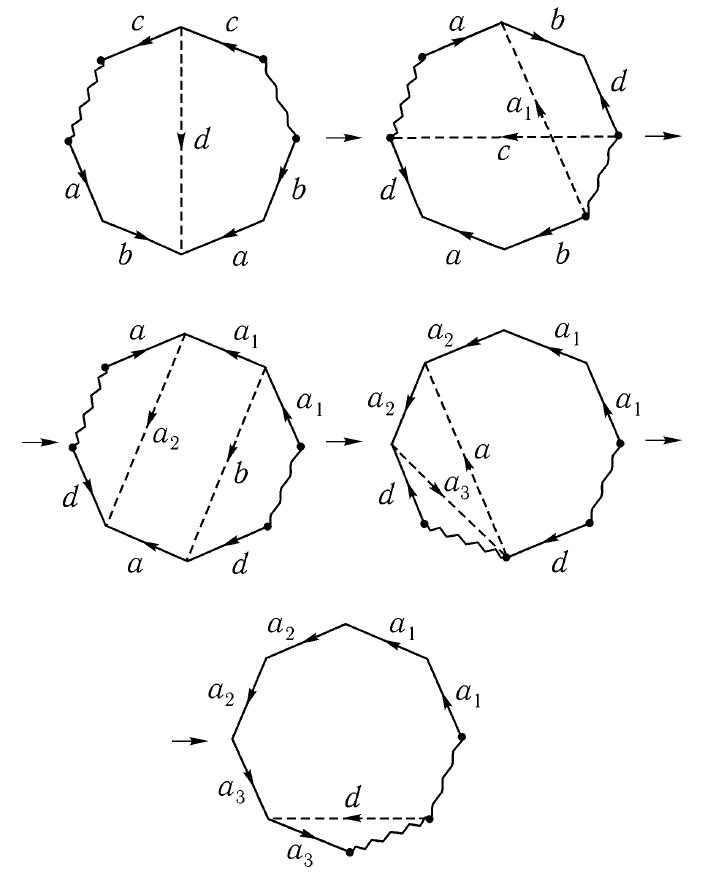
\includegraphics[width=\textwidth]{GaT-4.png}
            \caption{Замена ручек лентами Мёбиуса}
            \label{surface_typisation_picture_6}
            \todo[inline]{Перерисовать.}
        \end{figure}
    \end{proof}

    \begin{theorem}[без доказательства]
        Все поверхности, задаваемые каноническими развертками I и II типа попарно различны (не гомеоморфны).
    \end{theorem}

    \subsection{Классификация одномерных замкнутых многообразий.}

    \begin{theorem}
        Всякое связное замкнутое 1-многообразие гомеоморфно $S^1$.
    \end{theorem}

    \begin{proof}
        \begin{thlemma}
            Пусть $M$ --- 1-многообразие, $U$ и $V$ --- открытые подмножества $M$, каждое гомеоморфно $\RR$. Если $U \cap V \neq \varnothing$, то $U \cup V$ гомеоморфно либо $\RR$, либо $S^1$.
        \end{thlemma}

        \begin{proof}
            Зафиксируем гомеоморфизмы: $\varphi: U \to (0; 1)$, $\psi: V \to (0; 1)$, используя гомеоморфность $\RR$ и $(0; 1)$. Обозначим $A = \varphi(U \cap V)$, $B = \psi(U \cap V)$. Тогда $f = \psi \circ \varphi^{-1}$ --- гомеоморфизм между $A$ и $B$. Т.к. $A$ и $B$ --- открытые подмножества в $(0; 1)$ (а, значит, и в $\RR$), то каждое из них есть дизъюнктное объединение интервалов в $(0; 1)$.
            
            Пусть $I \subseteq A$ и $J \subseteq B$ ---  такие интервалы, что $f(I) = J$. Гомеоморфизм интервалов --- строго монотонное отображение. Он дает соответствие между концами интервалов. Пусть $x$ --- конец интервала $I$, $y$ --- конец интервала $J$, они соответствуют друг другу относительно $f$. Тогда хотя бы одна из этих точек --- конец интервала $(0; 1)$. Действительно, если обе внутренние, то точки $\varphi^{-1}(x)$ и $\psi^{-1}(y)$ нельзя отделить окрестностями в $M$, что противоречит хаусдорфовости.

            Таким образом для всякой такой пары интервалов $I$ и $J$ есть только два варианта (с точностью до перестановки и
            переворачивания):
            \begin{multicols}{2}
                \begin{enumerate}
                    \item $I = (a; b)$, $J = (0; 1)$.
                    \item $I = (a; 1)$, $J = (0; b)$.
                \end{enumerate}
            \end{multicols}
            В первом случае $V \subseteq U$, поэтому $V \cup U = U \simeq \RR$. Во втором случае таких пар интервалов либо одна, либо две. Если одна, то $U \cup V \simeq \RR$. Если две пары, то $U \cup V \simeq S^1$.
        \end{proof}

        В силу компактности, $M$ покрывается конечным набором открытых множеств, каждое из которых гомеоморфно $\RR$. Рассмотрим такое покрытие с минимальным числом элементов. Среди элементов покрытия найдутся два пересекающихся, обозначим их $U$ и $V$. Действительно, если любые два элемента покрытия не пересекаются, то $M$ либо не связно (если элементов покрытия хотя бы два), либо $M$ гомеоморфно $\RR$ (если элемент покрытия ровно один), т.е. не компактно.
        
        Если $U \cup V$ гомеоморфно $\RR$. Тогда в нашем покрытии можно заменить два элемента --- $U$ и $V$ --- на один элемент $U \cup V$, что противоречит минимальности покрытия. Значит по лемме $U \cup V$ гомеоморфно $S^1$.
        
        Опишем свойства $U \cup V$:
        \begin{multicols}{3}
            \begin{enumerate}
                \item компактно (т.к. $S^1$);
                \item замкнуто (компакт в хаусдорфовом пр-ве);
                \item открыто.
            \end{enumerate}
        \end{multicols}
        Тогда в силу связности $U \cup V = M$.
    \end{proof}

    \section{Геометрия}

    \subsection{Аффинные пространства}

    \begin{definition}
        \emph{Аффинное пространство (АП)} --- тройка $(X, \overrightarrow{X}, {+})$, где
        \begin{itemize}
            \item $X$ --- непустое множество, элементы которого называются \emph{точками},
            \item $\overrightarrow{X}$ --- векторное пространство над полем $\RR$, которое называется \emph{присоединённое векторное пространство},
            \item ${+}: X \times \overrightarrow{X} \to X$ --- операция ``откладывания вектора от точки'', которая удовлетворяет следующим аксиомам.
                \begin{enumerate}
                    \item Для всяких точек $x$ и $y$ есть единственный вектор $v \in \overrightarrow{X}$ такой, что $x + v = y$. Вектор $v$ обозначается как $\overrightarrow{xy}$ или $y - x$ и называется \emph{вектором между точками}.
                    \item $\forall x \in X, v, u \in \overrightarrow{X}\qquad x + (v + u) = (x + v) + u$.
                \end{enumerate}
        \end{itemize}

        Для краткости будем обозначать это аффинное пространство как просто $X$.
    \end{definition}

    \begin{example}
        Пусть $V$ --- векторное пространство, а $+$ --- операция сложения векторов в нём. Тогда $(V, V, {+})$ будет аффинным пространством.
    \end{example}

    \begin{lemma}
        Для любых точек $x$, $y$, $z$ аффинного пространства $X$ верно, что
        \begin{enumerate}
            \item $x + \overrightarrow{xy} = y$;
            \item $\overrightarrow{xy} + \overrightarrow{yz} = \overrightarrow{xz}$;
            \item $\overrightarrow{xx} = \overrightarrow{0}$;
            \item $x + \overrightarrow{0} = x$;
            \item $\overrightarrow{yx} = - \overrightarrow{xy}$;
            \item $\overrightarrow{xy} = \overrightarrow{0} \Rightarrow x = y$.
        \end{enumerate}
    \end{lemma}

    \begin{lemma}
        Пусть $o$ --- какая-то точка $X$. Рассмотрим отображение
        \[\varphi_o: X \to \overrightarrow{X}, x \mapsto \overrightarrow{ox}.\]
        Тогда $\phi_o$ --- биекция.
    \end{lemma}

    \begin{definition}
        Эта биекция называется \emph{векторизацией} аффинного пространства.
    \end{definition}

    % \subsubsection{Линейная и барицентрическая комбинации}

    \begin{definition}
        \emph{Линейной комбинацией $\sum_{i=1}^n t_i p_i$ точек $p_1, \dots, p_n \in X$ с коэффициентами $t_1, \dots, t_n$ относительно начала отсчёта $o \in X$} называется либо вектор
        \[v = \sum_{i=1}^n t_i \overrightarrow{op_i},\]
        либо точка
        \[p = o + v.\]

        Линейная комбинация называется:
        \begin{itemize}
            \item \emph{барицентрической}, если $\sum_{i=1}^n t_i = 1$;
            \item \emph{сбалансированной}, если $\sum_{i=1}^n t_i = 0$;
        \end{itemize}
    \end{definition}

    \begin{theorem}\ 
        \begin{enumerate}
            \item Барицентрическая комбинации является точкой, независящей от начала отсчёта.
            \item Сбалансированная комбинации является вектором, независящем от начала отсчёта.
        \end{enumerate}
    \end{theorem}

    \begin{proof}
        Пусть даны два различных начала отсчёта $o_1$ и $o_2$.

        \begin{enumerate}
            \begin{multicols}{2}
                \item 
                    \begin{align*}
                        &\left(o_1 + \sum_{i=1}^n t_i \overrightarrow{o_1 p_i}\right) - \left(o_2 + \sum_{i=1}^n t_i \overrightarrow{o_2 p_i}\right)\\
                        =&(o_1 - o_2) + \sum_{i=1}^n t_i (\overrightarrow{o_1 p_i} - \overrightarrow{o_2 p_i})\\
                        =&\overrightarrow{o_2 o_1} + \sum_{i=1}^n t_i \overrightarrow{o_1 o_2}\\
                        =&\overrightarrow{o_2 o_1} \left(1 - \sum_{i=1}^n t_i\right)\\
                        =&\overrightarrow{0}
                    \end{align*}
                \item 
                    \begin{align*}
                        &\sum_{i=1}^n t_i \overrightarrow{o_1 p_i} - \sum_{i=1}^n t_i \overrightarrow{o_2 p_i}\\
                        =&\sum_{i=1}^n t_i (\overrightarrow{o_1 p_i} - \overrightarrow{o_2 p_i})\\
                        =&\sum_{i=1}^n t_i \overrightarrow{o_1 o_2}\\
                        =&\overrightarrow{o_1 o_2} \sum_{i=1}^n t_i\\
                        =&\overrightarrow{0}
                    \end{align*}
            \end{multicols}
        \end{enumerate}
    \end{proof}

    \begin{definition}
        Множество $Y \subseteq X$ --- \emph{аффинное подпространство}, если есть линейное подпространство $V$ пространства $\overrightarrow{X}$ и точка $p \in X$, что
        \[Y = p + V := \{p + v \mid v \in V\}.\]
        $V$ называется \emph{направлением} $Y$.
    \end{definition}

    \begin{lemma}
        Пусть $Y = p + V$ --- аффинное подпространство.
        \begin{enumerate}
            \item Для любой точки $q \in Y$ верно, что $q + V = Y$.
            \item $Y$ --- аффинное пространство с $\overrightarrow{Y} = V$.
            \item Для любой точки $q \in Y$ верно, что $\varphi_q(Y) = V$.
        \end{enumerate}
    \end{lemma}

    \begin{definition}
        \emph{Размерность} аффинного пространства $\dim(X) := \dim(\overrightarrow{X})$.
    \end{definition}

    \begin{definition}
        \emph{Параллельный перенос} на вектор $v \in \overrightarrow{X}$ --- отображение
        \[T_v: X \to X, x \mapsto x + v.\]
    \end{definition}

    \begin{lemma}\ 
        \begin{enumerate}
            \item $T_{u + v} = T_u \circ T_v$.
            \item $T_{\overrightarrow{0}} = \Id$.
            \item $T_v$ --- биекция.
            \item $T_v^{-1} = T_{-v}$.
        \end{enumerate}
    \end{lemma}

    \begin{corollary}
        Параллельные переносы образуют группу, которая естественно изоморфна аддитивной группе $\overrightarrow{X}$.
    \end{corollary}

    \begin{definition}
        Аффинные подпространства одинаковой размерности \emph{параллельны}, если их направления совпадают.
    \end{definition}

    \begin{lemma}\ 
        \begin{enumerate}
            \item Два пространства параллельны тогда и только тогда, когда одно из них получается из другого параллельным переносом.
            \item $X$ разбивается на аффинные подпространства, параллельные данному $Y$.
        \end{enumerate}
    \end{lemma}

    \begin{definition}
        \emph{Прямая} --- аффинное подпространство размерности $1$.

        \emph{Гиперплоскость} в $X$ --- аффинное подпространство размерности $\dim(X) - 1$.
    \end{definition}

    \begin{theorem}
        Пересечение любого семейства аффинных подпространств есть либо пустое множество, либо аффинное подпространство.
    \end{theorem}

    \begin{proof}
        Пусть дано семейство $\Sigma$ аффинных подпространств. Если они все пересекаются (т.е. пересечение непусто), то можно выделить общую точку $p$. Тогда каждое аффинное пространство $A \in \Sigma$ имеет вид $p + V_A$, следовательно
        \[\bigcap_{A \in \Sigma} A = \bigcap_{A \in \Sigma} p + V_A = p + \bigcap_{A \in \Sigma} V_A.\]
        Поскольку пересечение векторных подпространств есть векторное подпространство, то есть некоторое векторное подпространство $U = \bigcap_{A \in \Sigma} V_A$, следовательно $\bigcap_{A \in \Sigma} A = p + U$, т.е. аффинное подпространство.
    \end{proof}

    \begin{definition}
        \emph{Аффинная оболочка} непустого множества $A \subseteq X$ --- пересечение всех аффинных подпространств, содержащих $A$. Обозначение: $\Aff(A)$.
    \end{definition}

    \begin{remark}
        $\Aff(A)$, как следует из теоремы, минимальное по включению аффинное пространство, содержащее $A$ как подмножество.
    \end{remark}

    \begin{theorem}\label{affin-hull-lower-definition}
        $\Aff(A)$ есть множество всех барицентрических комбинаций точек из $A$, т.е.
        \[\Aff(A) = \left\{\sum_{i=1}^n t_i a_i \mid n \in \NN \setminus \{0\} \wedge \{a_i\}_{i=1}^n \subseteq A \wedge \{t_i\}_{i=1}^n \subseteq \RR \wedge \sum_{i=1}^n t_i = 1\right\}\]
    \end{theorem}

    \begin{proof}
        Возьмём в качестве начала отсчёта любую точку $o$ из $A$. Тогда всякая барицентрическая комбинация $\sum_{i=1}^n t_i a_i$ точек из $A$ будет равна
        \[\sum_{i=1}^n t_i (o + v_i) = o + \sum_{i=1}^n t_i v_i\]
        При этом если вместо этого взять набор точек $\{a_1; \dots; a_n; o\}$, то $t_{n+1} = 1 - \sum_{i=1}^n t_i$, т.е. множество всех барицентрических комбинаций превратится в множество всех линейных комбинаций векторов из $A - o = \{a - o \mid a \in A\}$, т.е. линейной оболочкой $A - o$.
        
        С другой стороны $\Aff(A) - o$ есть пересечение всех векторных подпространств, содержащих $A - o$, т.е. тоже является линейной оболочкой $A - o$. Таким образом наши объекты совпали.
    \end{proof}

    \begin{definition}
        Множество точек $A$ называется \emph{аффинно зависимым}, если для некоторого $n \in \NN \setminus \{0\}$ существуют точки $a_1, \dots, a_n \in A$ и коэффициенты $t_1, \dots, t_n \in \RR \setminus \{0\}$, что
        \[\sum_{i=1}^n t_i = 0\qquad \text{ и }\qquad \sum_{i=1}^n t_i p_i = \overrightarrow{0}\]
        В противном случае множество называется \emph{аффинно независимым}.

        Также говорят, что сами точки \emph{аффинно (не)зависимы}, если их множество аффинно (не)зависимо.
    \end{definition}

    \begin{theorem}
        Пусть дано непустое $A \subseteq X$. TFAE
        \begin{enumerate}
            \item $A$ аффинно независимо.
            \item Каждая из точек $A$ не представляется в виде конечной барицентрической комбинации остальных.
            \item Каждая из точек $A$ не лежит в аффинной оболочке остальных точек $A$.
            \item При выделенной точке $a \in A$ множество векторов $\{a' - a \mid a' \in A \setminus \{a\}\}$ линейно независимо.
            \item Каждая из точек $\Aff(A)$ единственным образом представляется в виде конечной барицентрической комбинации точек из $A$.
        \end{enumerate}
    \end{theorem}

    \begin{proof}
        \begin{itemize}
            \item[$1 \Rightarrow 2$)] Пусть какая-то точка $a$ выражается в виде барицентрической комбинации точек $b_1$, \dots, $b_n$:
                \[a = \sum_{i=1}^n t_i b_i\]
                Тогда мы имеем, что нетривиальная сбалансированная комбинация $a - \sum_{i=1}^n t_i b_i$ равна $\overrightarrow{0}$. Удаляя слагаемые с нулевыми коэффициентами (если таковые есть), получаем противоречие с аффинной независимостью.

            \item[$1 \Leftarrow 2$)] Пусть дана есть точки $a_1, \dots, a_n \in A$ и коэффициенты $t_1, \dots, t_n \in \RR \setminus \{0\}$, что
                \[\sum_{i=1}^n t_i = 0\qquad \text{ и }\qquad \sum_{i=1}^n t_i p_i = \overrightarrow{0}.\]
                Тогда $n > 1$ и следовательно
                \[a_1 = \sum_{i=2}^n \frac{-t_i}{t_1} a_i\]

            \item[$2 \Leftrightarrow 3$)] По теореме \ref{affin-hull-lower-definition} имеем, что $A$ аффинно независимо тогда и только тогда, когда если никакая точка не представляется в виде барицентрической комбинации остальных, тогда и только тогда, когда она не лежит в афинной оболочке остальных.

            \item[$1 \Leftrightarrow 4$)] Любая нетривиальная сбалансированная комбинация точек из $A$ равна $\overrightarrow{0}$ тогда и только тогда, когда нетривиальная сбалансированная комбинация векторов в них из $a$ равна $\overrightarrow{0}$. Таким образом $A$ аффинно зависимо тогда и только тогда, когда какая-то нетривиальная линейная комбинация векторов из $a$ в некоторые другие точки равна $\overrightarrow{0}$, что равносильно линейной зависимости $\{a' - a \mid a' \in A \setminus \{a\}\}$.

            \item[$1 \Leftrightarrow 5$)] Какая-то точка $\Aff(A)$ представляется в виде двух различных барицентрических комбинаций точек из $A$ тогда и только тогда, когда есть нетривиальная сбалансированная комбинация точек из $A$. Соответственно каждая точка $\Aff(A)$ единственным образом представляется в виде барицентрической комбинации точек из $A$ тогда и только тогда, когда $A$ аффинно независимо.
        \end{itemize}
    \end{proof}

    \begin{theorem}
        Пусть дано конечное непустое $A \subseteq X$. Тогда $A$ аффинно независимо тогда и только тогда, когда $\dim(\Aff(A)) = |A| - 1$.
    \end{theorem}

    \begin{proof}
        Выделим из $A$ точку $a$ и определим
        \[A' := \{a' - a \mid a \in A \setminus \{a\}\}.\]
        Тогда $A$ аффинно независимо тогда и тогда только тогда, когда $A'$ линейно независимо. При этом размерность аффинной оболочки $A$ и линейной оболочки $A'$ совпадают; таким образом не более $|A'| = |A| - 1$. Таким образом $A$ аффинно независимо, если $\deg(\Aff(A)) = |A| - 1$.
    \end{proof}

    \begin{corollary}
        Для всякого (не обязательно конечного) множества $A \subseteq X$ верно неравенство
        \[\deg(\Aff(A)) \leqslant |A| + 1\]
    \end{corollary}

    \begin{definition}
        \emph{Аффинный базис (точечный базис)} --- максимальное по включению аффинно независимое множество. В частности, в $n$-мерном аффинном пространстве базис будет выглядеть как всякое аффинно независимое множество из $n+1$ точки.
    \end{definition}

    \begin{lemma}
        Пусть дано подмножество $A$ АП $X$.
        \begin{enumerate}
            \item Если $A$ --- аффинный базис $X$, то аффинная оболочка $A$ содержит в себя всё $X$.
            \item Если $A$ --- минимальное по включению множество, чья аффинная оболочка содержит всё $X$, то $A$ --- аффинный базис $X$.
        \end{enumerate} 
    \end{lemma}

    \begin{lemma}
        TFAE
        \begin{enumerate}
            \item $A$ --- аффинный базис $X$.
            \item $A$ имеет вид $\{a\} \cup \{a + e\}_{e \in A'}$, где $a \in X$, а $A'$ --- базис $\overrightarrow{X}$.
        \end{enumerate}
    \end{lemma}

    \begin{remark}
        Вследствие доказанной леммы также \emph{аффинным базисом} можно назвать любую точку $o \in X$ и базис $A'$ пространства $\overrightarrow{X}$.
    \end{remark}

    \begin{definition}
        Пусть $A = \{a_i\}_{i \in I}$ --- аффинный базис $X$, а $p$ --- любая точка $X$. Тогда $p$ единственным образом представляется в виде барицентрической комбинации
        \[p = \sum_{k=1}^n t_{i_k} a_{i_k}\]
        точек $A$ (остальные $t_i$ равны $0$). Следовательно последовательность $(t_i)_{i \in I}$ называется \emph{барицентрическими координатами $p$}.
    \end{definition}

    \begin{definition}
        Пусть $o$ --- начало отсчёта в $X$, $\{e_i\}_{i \in I}$ --- базис $\overrightarrow{X}$, а $p$ --- любая точка $X$. Тогда $p$ единственным образом представляется в виде
        \[p = 0 + \sum_{k=1}^n x_{i_k} e_{i_k}\]
        (остальные $x_i$ равны $0$). Следовательно последовательность $(x_i)_{i \in I}$ называется \emph{аффинными координатами точки $p$}.
    \end{definition}

    \begin{lemma}\ 
        \begin{enumerate}
            \item Пусть $(t_i)_{i \in I}$ --- барицентрические координаты $p$ в аффинном базисе $\{a_i\}_{i \in I}$. Пусть также $j$ --- всякий индекс из $I$. Тогда $(t_i)_{i \in I \setminus \{j\}}$ --- аффинные координаты $p$ в базисе $\{a_i - a_j\}_{i \in I \setminus \{j\}}$ с центром отсчёта в $a_j$.
            \item Пусть $(x_i)_{i \in I}$ --- аффинные координаты $p$ в базисе $\{e_i\}_{i \in I}$ с центром отсчёта $o$. Тогда $(t_i)_{i \in I \cup \{j\}}$ --- барицентрические координаты $p$ в аффинном базисе $\{a_i\}_{i \in I \cup \{j\}}$, где $t_i = x_i$ и $a_i = o + e_i$ для всех $i \in I$, а $t_j = 1 - \sum_{i \in I} t_i$ и $a_j = o$.
        \end{enumerate}
    \end{lemma}

    \begin{theorem}
        Пусть даны АП $X$, $Y$ и точка $p \in X$. Любое отображение $F: X \to Y$ индуцирует отображение
        \[\widetilde{F}_p: \overrightarrow{X} \to \overrightarrow{Y}, v \mapsto F(p+v) - F(p)\]

        Тогда если для некоторой точки $p$ $\widetilde{F}_p$ линейно, то $\widetilde{F}_q = \widetilde{F}_p$ для всех $q \in X$.
    \end{theorem}

    \begin{proof}
        Пусть $r \in X$ и $v = r - q$. Пусть также $u = q - p$. Тогда
        \begin{align*}
            \widetilde{F}_q(v)
            &= F(r) - F(q)\\
            &= (F(r) - F(p)) - (F(q) - F(p))\\
            &= \widetilde{F}_p(r - p) - \widetilde{F}_p(q - p)\\
            &= \widetilde{F}_p((r - p) - (q - p))\\
            &= \widetilde{F}_p(r - q)\\
            &= \widetilde{F}_p(v)
        \end{align*}
    \end{proof}

    \begin{definition}
        Пусть даны АП $X$ и $Y$. Отображение $F: X \to Y$ называется \emph{аффинным}, если $\widetilde{F}$ является линейным. Причём $\widetilde{F}$ называется \emph{линейной частью аффинного отображения $F$}.
    \end{definition}

    \begin{lemma}
        Пусть дано отображение $F: X \to Y$. TFAE
        \begin{enumerate}
            \item $F$ аффинно.
            \item Существует линейное отображение $L: \overrightarrow{X} \to \overrightarrow{Y}$, что для любых $p, q \in X$
                \[F(p) - F(q) = L(p - q)\]
        \end{enumerate}
    \end{lemma}

    \begin{theorem}
        Пусть даны $x \in X$, $y \in Y$ и линейное $L: \overrightarrow{X} \to \overrightarrow{Y}$. Тогда существует единственное аффинное отображение $F: X \to Y$, что
        \[\widetilde{F} = L \text{ и } F(x) = y.\] 
    \end{theorem}

    \begin{proof}
        \begin{itemize}
            \item \textbf{Существование.} Определим
                $F: X \to Y, p \mapsto y + L(p - x).$
                Тогда понятно, что $\widetilde{F}_x = L$, а $F(x) = y$. Следовательно $F$ аффинно и удовлетворяет требуемым условиям.
            \item \textbf{Единственность.} Пусть даны $F$ и $G$ --- аффинные отображения, удовлетворяющие требуемым условиям. Следовательно для всякой точки $p \in X$
                \[F(p) = F(x) + \widetilde{F}(p - x) = y + L(p - x) = G(x) + \widetilde{G}(p - x) = G(p).\]
        \end{itemize}
    \end{proof}

    \begin{corollary}
        Пусть даны $x \in X$, $y \in Y$, базис $\{e_i\}_{i \in I}$ пространства $\overrightarrow{X}$ и множество $\{g_i\}_{i \in I}$ векторов в $\overrightarrow{Y}$. Тогда существует единственное аффинное $F: X \to Y$, что
        \begin{itemize}
            \item $F(x) = y$,
            \item $\widetilde{F}(e_i) = g_i$ для всех $i \in I$.
        \end{itemize}
    \end{corollary}

    \begin{corollary}
        Пусть даны аффинный базис $\{x_i\}_{i \in I}$ в $X$ и подмножество $\{y_i\}_{i \in I}$ пространства $Y$. Тогда существует единственное аффинное отображение $F: X \to Y$, что $F(x_i) = y_i$ для всех $i \in I$.
    \end{corollary}

    \begin{lemma}
        Аффинные отображения сохраняют барицентрические комбинации, т.е. для всяких аффинного отображения $F: X \to Y$, множества точек $\{x_i\}_{i=1}^n \subseteq X$ и множества чисел $\{t_i\}_{i=1}^n$, что $\sum_{i=1}^n t_i = 1$ верно, что
        \[F\left(\sum_{i=1}^n t_i p_i\right) = \sum_{i=1}^n t_i F(p_i).\]
    \end{lemma}

    \begin{proof}
        Пусть $x \in X$. Тогда
        \begin{align*}
            F\left(\sum_{i=1}^n t_i p_i\right)
            &= F\left(x + \sum_{i=1}^n t_i (p_i - x)\right)&
            &= F(x) + \widetilde{F}\left(\sum_{i=1}^n t_i (p_i - x)\right)\\
            &= F(x) + \sum_{i=1}^n t_i \widetilde{F}(p_i - x)&
            &= F(x) + \sum_{i=1}^n t_i (F(p_i) - F(x))\\
            &= \sum_{i=1}^n t_i F(p_i)&
        \end{align*}
    \end{proof}

    \begin{corollary}
        Для всякого $A \subseteq X$
        \[F(\Aff(A)) = \Aff(F(A))\]
    \end{corollary}

    \begin{lemma}
        Композиция аффинных отображений --- аффинное отображение. При этом линейная часть композиции --- композиция линейных частей.
    \end{lemma}

    \begin{proof}
        Пусть даны аффинные отображения $F: Y \to Z$, $F: X \to Y$. Тогда
        \[
            (F \circ G)(x) - (F \circ G)(y)
            = \widetilde{F}(G(x) - G(y))
            = (\widetilde{F} \circ \widetilde{G})(x - y)
        \]
        Следовательно $F \circ G$ аффинно и $\widetilde{F \circ G} = \widetilde{F} \circ \widetilde{G}$.
    \end{proof}

    \begin{theorem}
        Пусть дано аффинное $F: X \to Y$.
        \begin{enumerate}
            \item Образ аффинного подпространства $X$ по $F$ есть аффинное подпространство $Y$.
            \item Прообраз аффинного подпространства $Y$ по $F$ есть аффинное пространство $X$ или пустое множество.
        \end{enumerate}
    \end{theorem}

    \begin{proof}\ 
        \begin{enumerate}
            \item Пусть $A$ --- аффинное подпространство $X$. Тогда
                \[F(A) = F(\Aff(A)) = \Aff(F(A)),\]
                т.е. аффинное подпространство $Y$.
            \item Пусть $B$ --- аффинное подпространство $Y$, а $A := F^{-1}(B)$. Тогда
                \[F(\Aff(A)) = \Aff(F(A)) = \Aff(B) = B,\]
                т.е. $\Aff(A) \subseteq F^{-1}(B) = A$, следовательно $A = \Aff(A)$, т.е. является аффинным подпространством $X$.
        \end{enumerate}
    \end{proof}

    \begin{theorem}
        Класс параллельных переносов в $X$ совпадает с классом аффинных отображений $X$ на себя с тождественной линейной частью.
    \end{theorem}

    \begin{proof}\ 
        \begin{itemize}
            \item Пусть $F$ --- параллельный перенос в $X$ на вектор $v$. Тогда для всяких точек $p, q \in X$ верно, что
                \[
                    F(p) - F(q)
                    = (p + v) - (q + v)
                    = p - q
                    = \Id(p - q)
                \]
                Следовательно $F$ --- аффинное отображение, а $\widetilde{F} = \Id$.
            \item Пусть $F$ --- аффинное преобразование, что $\widetilde{F} = \Id$. Зафиксируем точку $p \in X$. Тогда для всякой точки $q \in X$
                \[
                    F(q) - q
                    = (F(q) - F(p)) + (F(p) - p) + (p - q)
                    = (\widetilde{F}(q-p) - (q-p)) + F(p) - p
                    = F(p) - p
                \]
                Следовательно $F(q) = q + v$, где $v := F(p) - p$.
        \end{itemize}
    \end{proof}

    \begin{definition}
        Аффинное отображение $F: X \to X$, что $\widetilde{F} = k \Id$ для некоторого коэффициента $k \notin \{0, 1\}$, называется \emph{гомотетией}, а $k$ называется \emph{коэффициентом растяжения} гомотетии $F$.
    \end{definition}

    \begin{theorem}
        Гомотетия имеет ровно одну неподвижную точку.
    \end{theorem}

    \begin{proof}
        \begin{itemize}
            \item \textbf{Существование.} Зафиксируем точку $p \in X$ и рассмотрим произвольную $q \in X$. Тогда
                \[
                    F(q)
                    = F(p + \overrightarrow{pq})
                    = F(p) + k\overrightarrow{pq}
                    = p + \overrightarrow{pF(p)} + k\overrightarrow{pq}
                    = q + \overrightarrow{pF(p)} - (1-k)\overrightarrow{pq}
                \]
                Следовательно $F(q) = q$ тогда и только тогда, когда $\overrightarrow{pF(p)} = (1-k)\overrightarrow{pq}$. Тогда определим
                \[
                    q := p + \frac{\overrightarrow{pF(p)}}{1-k}
                \]
                В таком случае условие выполнится, и тогда $F(q) = q$.
            \item \textbf{Единственность.} Пусть $p$ и $q$ --- неподвижные точки $F$. Следовательно
                \[
                    \widetilde{F}(p-q)
                    = F(p) - F(q)
                    = p - q
                    = 1 \cdot \Id(p - q)
                \]
                т.е. $k = 1$ --- противоречие.
        \end{itemize}
    \end{proof}

    \begin{definition}
        Неподвижная точка гомотетии называется \emph{центром гомотетии}.
    \end{definition}

    \begin{theorem}[основная теорема аффинной геометрии]\label{main-affine-theorem}
        Пусть $X$, $Y$ --- аффинные пространства (над $\RR$), $\dim X \geqslant 2$. Пусть $F: X \to Y$ --- инъективное отображение, переводящее прямые в прямые. Тогда $F$ аффинно.
    \end{theorem}

    \begin{proof}
        Будем обозначать прямую, проходящую чрез $a$ и $b$ за $(ab)$, а параллельность прямых $l_1$ и $l_2$ за $l_1 \parallel l_2$.

        \begin{thlemma}\label{main-affine-theorem-thlemma-1}
            Пусть $X$ --- АП, $\dim X \geqslant 2$. $l_1$ и $l_2$ --- параллельные прямые. Три различные точки: $a, b \in l_1$, $c \in l_2$. Пусть $l_3 = (ac)$, $b \in l_4$ и $l_3 \parallel l_4$.
            \begin{enumerate}
                \item Существует аффинная плоскость $\Sigma$, содержащая прямые $l_1$ и $l_2$.
                \item Прямые $l_3$ и $l_4$ также лежат в $\Sigma$.
                \item Прямые $l_2$ и $l_4$ пересекаются в одной точке, обозначим её $d$.
                \item $\overrightarrow{ab} = \overrightarrow{cd}$ и $\overrightarrow{ac} = \overrightarrow{bd}$.
                \item Прямые $l_5 = (ad)$ и $l_6 = (bc)$ лежат в $\Sigma$ и пересекаются в одной точке, обозначим её $o$.
            \end{enumerate}
        \end{thlemma}

        \begin{proof}
            \todo[inline]{TODO А надо ли?}
        \end{proof}

        \begin{thlemma}
            $F$ сохраняет параллельность прямых, т.е. $l_1 \parallel l_2 \Leftrightarrow F(l_1) \parallel F(l_2)$.
        \end{thlemma}

        \begin{proof}
            Если $l_1$ и $l_2$ пересекаются, то и пересекаются и их образы. И наоборот: если их образы пересекаются, то и сами прямые пересекаются в точке, являющейся прообразом пересечением.

            Следовательно $F$ сохраняет непересекаемость прямых. Также заметим, что по лемме \ref{main-affine-theorem-thlemma-1} есть пересекающиеся (различные) прямые $l_5$ и $l_6$, пересекающиеся с $l_1$ и $l_2$ в разных точка. Следовательно их образами будут пересекающиеся прямые $l_5'$ и $l_6'$, пересекающиеся с образами $l_1$ и $l_2$ --- $l_1'$ и $l_2'$ --- в разных точках, следовательно $l_1'$ и $l_2'$ будут лежать в плоскости, порождённой $l_5'$ и $l_6'$. Следовательно будут параллельны, так как не пересекаются.
        \end{proof}

        \begin{thlemma}
            Зафиксируем $a \in X$. Рассмотрим
            \[\widetilde{F}_a: \overrightarrow{X} \to \overrightarrow{Y}, v \mapsto F(a + v) - F(a).\]
            Тогда $\widetilde{F}_a$ аддитивно.
        \end{thlemma}

        \begin{proof}
            Пусть даны неколлинеарные ненулевые вектора $u$ и $v$. Рассмотрим $b := a + u$, $c := a + v$. По лемме \ref{main-affine-theorem-thlemma-1} есть $d := a + u + v$. Тогда $F((ab)) \parallel F((cd))$, $F((ac)) \parallel F((bd))$, следовательно $F(b) - F(a) = F(d) - F(c)$. Значит
            \begin{multline*}
                    \widetilde{F}_a(u) + \widetilde{F}_a(v)
                    = (F(b) - F(a)) + (F(c) - F(a))\\
                    = (F(d) - F(c)) + (F(c) - F(a))
                    = F(d) - F(a)
                    = \widetilde{F}_a(u + v)
            \end{multline*}

            Теперь же пусть даны коллинеарные $u$ и $w$. Возьмём всякий неколлинеарный им $v$, и тогда
            \[
                \widetilde{F}_a(u+w) + \widetilde{F}_a(v)
                = \widetilde{F}_a(u + w + v)
                = \widetilde{F}_a(u) + \widetilde{F}_a(w + v)
                = \widetilde{F}_a(u) + \widetilde{F}_a(w) + \widetilde{F}_a(v),
            \]
            а значит $\widetilde{F}_a(u + w) = \widetilde{F}_a(u) + \widetilde{F}_a(w)$.
        \end{proof}

        \begin{thlemma}
            $\widetilde{F}_a$ не зависит от $a$.
        \end{thlemma}

        \begin{proof}
            Пусть даны точки $a$ и $b$ и вектор $v$. Тогда
            \[
                \widetilde{F}_b(v) = F(b+v) - F(b)
                = (F(a + \overrightarrow{ab} + v) - F(a)) - (F(b) - F(a))
                = \widetilde{F}_a(\overrightarrow{ab} + v) - \widetilde{F}_a(\overrightarrow{ab})
                = \widetilde{F}_a(v)
            \]
        \end{proof}

        Поэтому можно рассматривать общую $\widetilde{F}$.

        \begin{thlemma}
            Для всякого $k \in \QQ$ и вектора $v$ верно, что
            \[\widetilde{F}(kv) = k \widetilde{F}(v)\]
        \end{thlemma}

        \begin{proof}
            \begin{enumerate}
                \item Если $k = -1$, то
                    \[
                        \widetilde{F}(-u)
                        = \widetilde{F}(-u) + \widetilde{F}(u) - \widetilde{F}(u)
                        = \widetilde{F}(-u + u) - \widetilde{F}(u)
                        = \widetilde{F}(0) - \widetilde{F}(u)
                        = 0 - \widetilde{F}(u)
                        = -\widetilde{F}(u)
                    \]
                \item Если $k \in \NN$, то
                    \[
                        \widetilde{F}(kv)
                        = \widetilde{F}(\underbrace{v + \dots + v}_{k \text{ раз}})
                        = \underbrace{F(v) + \dots + F(v)}_{k \text{ раз}}
                        = k \widetilde{F}(v)
                    \]
                \item Если $k = -n$, где $n \in \NN$, то
                    \[
                        \widetilde{F}(-nv)
                        = -\widetilde{F}(nv)
                        = -n\widetilde{F}(v)
                    \]
                \item Если $k = 1/n$, где $n \in \NN$, то
                    \[
                        \widetilde{F}\left(\frac{1}{n}v\right)
                        = \frac{1}{n} \cdot n \cdot \widetilde{F}\left(\frac{1}{n}v\right)
                        = \frac{1}{n} \cdot \widetilde{F}\left(n \cdot \frac{1}{n}v\right)
                        = \frac{1}{n} \widetilde{F}(v)
                    \]
                \item Если $k = n/m$, где $n \in \ZZ$, а $m \in \NN$, то
                    \[
                        \widetilde{F}\left(\frac{n}{m}v\right)
                        = n\widetilde{F}\left(\frac{1}{m}v\right)
                        = \frac{n}{m}\widetilde{F}(v)
                    \]
            \end{enumerate}
        \end{proof}

        \begin{thlemma}
            Для всяких $\lambda \in \RR$ и ненулевого вектора $u$ $\widetilde{F}(\lambda u)$ коллинеарен $\widetilde{F}(u)$ и $\widetilde{F}(\lambda u) / \widetilde{F}(u)$.
        \end{thlemma}

        \begin{proof}
            Коллинеарность следует из того, что прямая переходит в прямую. Теперь пусть имеется два ненулевых коллинеарных вектора $u$ и $v$. Рассмотрим им неколлинеарный вектор $w$. Отложим от любой точки $a$ вектора:
            \begin{align*}
                x_1 &:= a + u,&
                x_2 &:= a + \lambda u,&
                y_1 &:= a + v,&
                y_2 &:= a + \lambda v,&
                z_1 &:= a + w,&
                z_2 &:= a + \lambda w.
            \end{align*}

            Поскольку гомотетия с центром в $a$ и коэффициентом $\lambda$ переводит $x_1$ в $x_2$, $y_1$ в $y_2$ и $z_1$ в $z_2$, то $(x_1y_1) \parallel (x_2y_2)$, $(z_1y_1) \parallel (z_2y_2)$.

            Пусть $a'$, $x_1'$, $x_2'$, $y_1'$, $y_2'$, $z_1'$, $z_2'$ являются образами по $F$ точек $a$, $x_1$, $x_2$, $y_1$, $y_2$, $z_1$, $z_2$. Тогда $(x_1'y_1') \parallel (x_2'y_2')$, $(z_1'y_1') \parallel (z_2'y_2')$. При этом $a'$, $x_1'$, $x_2'$, $z_1'$ и $z_2'$ лежат на одной прямой, а $a'$, $y_1'$ и $y_2'$ --- на другой. Следовательно гомотетия с центром в $a'$ и коэффициентом $\overrightarrow{a'y_2'}/\overrightarrow{a'y_1'}$ переводит $y_1'$ в $y_2'$ и оставляет прямые параллельными, значит переводит $x_1'$ в $x_2'$ и $z_1'$ в $z_2'$. Следовательно
            \[
                \frac{\widetilde{F}(\lambda v)}{\widetilde{F}(v)}
                = \frac{\overrightarrow{a'x_2'}}{\overrightarrow{a'x_1'}}
                = \frac{\overrightarrow{a'y_2'}}{\overrightarrow{a'y_1'}}
                = \frac{\overrightarrow{a'z_2'}}{\overrightarrow{a'z_1'}}
                = \frac{\widetilde{F}(\lambda u)}{\widetilde{F}(u)}
            \]
        \end{proof}

        Рассмотрим любую прямую $m$ и введём на $m$ и на $m' := F(m)$ аффинные координаты, так, что $F$ переводит $0$ в $0$ и $1$ в $1$. Пусть $\alpha: \RR \to \RR$ является сужением $F$ на $m$ описанным в данных координатных системах. Тогда по доказанным леммам мы имеем, что
        \begin{itemize}
            \item $\alpha(0) = 0$;
            \item $\alpha(1) = 1$;
            \item $\forall q \in \QQ, x \in \RR \quad \alpha(qx) = q \alpha(x)$;
            \item $\forall \lambda, x, y \in \RR \quad \frac{\alpha(\lambda x)}{\alpha(x)} = \frac{\alpha(\lambda y)}{\alpha(y)}$;
            \item $\forall x, y \in \RR \quad \alpha(x + y) = \alpha(x) + \alpha(y)$.
        \end{itemize}

        \begin{thlemma}
            Для всяких $x, y \in \RR$ верно, что $\alpha(xy) = \alpha(x) \alpha(y)$. 
        \end{thlemma}

        \begin{proof}
            Если $x = 0$, то
            \[
                \alpha(xy)
                = \alpha(0y)
                = \alpha(0)
                = 0
                = \alpha(0) \alpha(y)
                = \alpha(x) \alpha(y);
            \]
            аналогично если $y = 0$.

            Иначе же
            \[
                \alpha(xy)
                = \alpha(x) \cdot \frac{\alpha(xy)}{\alpha(x)}
                = \alpha(x) \cdot \frac{\alpha(y)}{\alpha(1)}
                = \alpha(x) \cdot \alpha(1)
            \]
        \end{proof}

        Тогда мы имеем, что для всякого многочлена $P$ с рациональными коэффициентами и всякой величины $r \in \RR$ мы имеем, что
        \[\alpha(P(r)) = P(\alpha(r))\]
        В частности, все числа, представимые в виде квадратов вещественных чисел, остаются представимыми. Значит неотрицательные числа $\alpha$ переводит в неотрицательные, а значит неположительные в неположительные. Следовательно $\alpha$ сохраняет порядок на $\RR$. При этом на $\QQ$ $\alpha$ тождественна. Следовательно из принципа вложенных отрезков выходит тождественность $\alpha$ на всё $\RR$.

        Следовательно $\widetilde{F}$ линейна, значит $F$ аффинна.
    \end{proof}

    \subsection{Проективные пространства}

    \begin{definition}
        Пусть $V$ --- векторное пространство над полем $K$. Введём на множестве $V \setminus \{0\}$ отношение эквивалентности
        \[x \sim y :\Leftrightarrow \exists \lambda \in K: x = \lambda y.\]
        Тогда $(V \setminus \{0\}) / \sim$ --- \emph{проективное пространство}, порождённое векторным пространством $V$; обозначается $\PP(V)$.

        Отображение $P: V \setminus \{0\} \to \PP(V), v \mapsto [v]_{\sim}$ --- \emph{каноническая проекция} или \emph{проективизация}.

        Также $P(K^n)$ обозначается за $K P^n$.
    \end{definition}

    \begin{definition}
        Пусть $W$ --- нетривиальное подпространство векторного пространства $V$. Тогда $\PP(W)$ называется \emph{подпространством} $\PP(V)$.
    \end{definition}

    \begin{definition}
        \emph{Размерность} $\PP(V)$ равна $\dim(V) - 1$.
    \end{definition}

    \begin{theorem}\label{proj-subspaces-intersection-theorem}
        Пусть даны $Y$ и $Z$ --- подпространства проективного пространства $X$, что $\dim(Y) + \dim(Z) \geqslant \dim(X)$ (все пространства конечномерные). Тогда
        \begin{enumerate}
            \item $Y \cap Z \neq \varnothing$;
            \item $Y \cap Z$ --- подпространство;
            \item $\dim(Y \cap Z) \geqslant \dim(Y) + \dim(Z) - \dim(X)$.
        \end{enumerate}
    \end{theorem}

    \begin{proof}
        Пусть $X$, $Y$, $Z$ являются проективизациями $V_X$, $V_Y$ и $V_Z$ соответственно.
        \begin{enumerate}
            \item По определению $\dim(V_Y) + \dim(V_Z) \geqslant \dim(V_X) + 1$. Следовательно $V_Y \cap V_Z$ нетривиально, а значит $Y \cap Z \neq \varnothing$.
            \item $V_Y \cap V_Z$ есть нетривиальное подпространство $V_X$, значит $Y \cap Z$ есть подпространство $X$.
            \item
                \begin{multline*}
                    \dim(Y \cap Z)
                    = \dim(V_Y \cap V_Z) - 1\\
                    \geqslant \dim(V_Y) + \dim(V_Z) - \dim(V_X) - 1
                    = \dim(Y) + \dim(Z) - \dim(X)
                \end{multline*}
        \end{enumerate}
    \end{proof}

    \begin{theorem}
        Пересечение любого семейства проективных подпространств есть либо пустое множество, либо аффинное подпространство.
    \end{theorem}

    \begin{proof}
        Пусть дано семейство $\Sigma$ проективных подпространств. Каждое проективное пространство $A \in \Sigma$ является проективизацией некоторого векторного подпространства $V_A$. При этом понятно, что
        \[\bigcap_{A \in \Sigma} A = \bigcap_{A \in \Sigma} \PP(V_A) = \PP\left(\bigcap_{A \in \Sigma} V_A\right).\]
        Поскольку пересечение векторных подпространств есть векторное подпространство, то есть некоторое векторное подпространство $U = \bigcap_{A \in \Sigma} V_A$, следовательно $\bigcap_{A \in \Sigma} A = \PP(U)$, т.е. проективное подпространство. При этом $U$ получается пустым тогда и только тогда, когда $U$ тривиально.
    \end{proof}

    \begin{definition}
        Пусть $X$ --- проективное пространство. \emph{Проективная оболочка} непустого подмножества $A \subseteq X$ --- пересечение всех проективных подпространств $X$, содержащих $A$.
    \end{definition}

    \begin{remark}
        Как следует из теоремы, проективная оболочка множества $A$ есть минимальное по включению проективное подпространство, содержащее $A$.
    \end{remark}

    \begin{lemma}
        Пусть дано всякое множество $A$ точек проективного пространства $X = \PP(V)$. Для всякого $a \in A$ обозначим за $v_a$ какой-нибудь вектор из $V$, каноническая проекция которого совпадает с $a$. Тогда проективная оболочка $A$ совпадает с проективизацией линейной оболочки $\{v_a\}_{a \in A}$.
    \end{lemma}

    \begin{proof}
        Пусть $Y = \PP(U)$ --- случайное подпространство $X$. Тогда понятно, что для всякой точки $a \in A$ верно, что $a \in Y \Leftrightarrow v_a \in U$. Поэтому $A \subseteq Y \Leftrightarrow \{v_a\}_{a \in A} \subseteq U$. Поэтому пересечение всех проективных подпространств, содержащих $A$, является проективизацией пересечения всех векторных подпространств, содержащих $\{v_a\}_{a \in A}$. А это и значит, что проективная оболочка $A$ совпадает с проективизацией векторной оболочки $\{v_a\}_{a \in A}$.
    \end{proof}

    \begin{definition}
        Пусть $X = \PP(V)$ --- проективное пространство размерности $n$. \emph{Проективный базис} $X$ --- множество из $n+2$ точек, никакие $n+1$ из которых не лежат в одной гиперплоскости.
    \end{definition}

    \begin{lemma}
        Пусть дан базис $P = \{p_i\}_{i=1}^{n+2}$ проективного пространства $X = \PP(V)$. Тогда существует такой набор $\{v_i\}_{i=1}^{n+2}$ векторов из $V$, что $p_i$ будет канонической проекцией $v_i$, а $v_{n+2} = \sum_{i=1}^{n+1} v_i$.
    \end{lemma}

    \begin{proof}
        Рассмотрим набор $E = \{e_i\}_{i=1}^{n+1}$ векторов из $V$, что $p_i$ является канонической проекцией $e_i$. Поскольку проективная оболочка $\{p_i\}_{i=1}^{n+1}$ совпадает со всем $X$, то линейная оболочка $E$ совпадает с $V$, а значит $E$ --- базис $V$. Выберем любой вектор $v_{n+2}$, канонической проекцией которого является $p_{n+2}$. Тогда $v_{n+2} = \sum_{i=1}^{n+1} \alpha_i e_i$. Заметим, что $\alpha_i \neq 0$ для каждого $i$, так как иначе линейная оболочка $E \setminus \{e_i\} \cup \{v_{n+2}\}$ не совпадает со всем $V$, а значит $P \setminus p_i$ лежит в какой-то гиперплоскости. Поэтому можно рассмотреть $v_i := \alpha_i e_i$. Тогда $p_i$ будет канонической проекцией $v_i$, а $v_{n+2} = \sum_{i=1}^{n+1} v_i$.
    \end{proof}

    \begin{definition}
        Пусть $X = \PP(V)$. Зафиксируем некоторый базис $\{e_i\}_{i \in I}$ пространства $V$. Для всякой точки $p$ есть семейство
        \[v \cdot (K \setminus \{0\}) = \{v \cdot \lambda \mid \lambda \in K \wedge \lambda \neq 0\} = P^{-1}(p).\]
        Пусть $(x_i)_{i \in I}$ --- координаты $v$ в выбранном базисе. Тогда $(\lambda x_i)_{i \in I}$ --- координаты $\lambda v$, значит координаты $p$ ``определены с точностью до пропорциональности''.

        Поэтому последовательность $(x_i)_{i \in I}$ с точностью до пропорциональности называется \emph{однородными координатами} точки $p$ и обозначается
        \[
            p = [x_i]_{i \in I}
            \quad \text{ или } \quad
            p = [x_0 : x_1 : \dots : x_n], \text{ где } n = \dim(X)
        \]
        В частности,
        \[
            [x_i]_{i \in I} = [y_i]_{i \in I}
            \quad \Longleftrightarrow \quad
            \exists \lambda \in K \setminus \{0\}:\ \forall i \in I\ y_i = \lambda x_i.
        \]
    \end{definition}

    \begin{definition}
        Пусть $X$ --- аффинное пространство. Зафиксируем $a \in X$ и определим стандартную векторизацию $X$ относительно $a$:
        \[\varphi_a: X \to \overrightarrow{X}, x \mapsto \overrightarrow{ax}.\]
        Рассмотрим векторное пространство $V := \overrightarrow{X} \times K$.

        $\widehat{X} := \PP(V)$ --- \emph{проективное пополнение АП $X$}. При этом всякой точке $x \in X$ соответствует точка с однородными координатами
        \[[\varphi_a(x) : 1],\]
        т.е. первые координаты взяты у $\varphi_a$, а последняя установлена равной $1$. При этом $X_\infty := \PP(\overrightarrow{X} \times \{0\})$ --- множество \emph{бесконечно удалённых точек}.
    \end{definition}

    \begin{lemma}\ 
        \begin{enumerate}
            \item $X_\infty$ --- гиперплоскость в $\widehat{X}$. Она называется \emph{бесконечно удалённой гиперплоскостью}.
            \item Каждому аффинному подпространству $Y \subseteq X$ соответствует проективное подпространство $\widehat{Y} \subseteq \widehat{X}$.
            \item Каждое проективное подпространство в $\widehat{X}$ либо соответствует аффинному подпространству в $X$, либо содержится в бесконечно удалённой гиперплоскости.
        \end{enumerate}
    \end{lemma}

    \begin{example}
        $\RR P^n$ --- проективное пополнение $\RR^n$. Это видно из стандартного вложения
        \[\varphi: \RR^n \to \RR P^n, (x_1, \dots, x_n) \mapsto [x_1 : \dots : x_n : 1]\]
        При этом бесконечные удалённые точки --- те, у которых последняя из однородных координат равна $0$.
    \end{example}

    \begin{definition}
        Пусть $X = \PP(V)$ --- проективное пространство. Выберем в нём гиперплоскость $Y = \PP(U)$ и рассмотрим в $V$ аффинную гиперплоскость, параллельную $U$ и не проходящую через $0$. Тогда всякая прямая в $V$ либо лежит в $U$, либо пересекается с $W$ ровно в одной точке. Тем самым имеется биекция
        \[\pi: X \setminus Y \to W, x \mapsto P(x) \cap W\]
        называется \emph{аффинной картой пространства $\PP(V)$}.
    \end{definition}

    \begin{remark}\ 
        \begin{enumerate}
            \item $U = \overrightarrow{W}$.
            \item $X = \widehat{W}$.
            \item $Y = W_\infty$.
        \end{enumerate}
    \end{remark}

    \begin{theorem}
        Пусть $V$, $W$ --- векторные пространства и $L: V \mapsto W$ --- инъективное линейное отображение. Тогда существует единственное отображение $F: \PP(V) \to \PP(W)$, что коммутативна диаграмма
        \[
            \xymatrix{
                V \setminus \{0\} \ar[d]^{P_V} \ar[r]^{L} & W \setminus \{0\} \ar[d]^{P_W}\\
                {\PP}(V) \ar[r]^{F} & {\PP}(W)
            }
        \]
        где $P_V$ и $P_W$ --- проекции из $V \setminus \{0\}$ и $W \setminus \{0\}$ в $\PP(V)$ и $\PP(W)$ соответственно.
    \end{theorem}

    \begin{proof}
        Прообраз при $P_V$ всякой точки $a \in \PP(V)$ есть прямая в $V$, которая отображается при $L$ в прямую в $W$, а та при $P_W$ --- в точку в $\PP(W)$. Значит образ всякой точки $a$ при $F$ определён однозначно.
    \end{proof}

    \begin{definition}
        Отображение $F$ из теоремы называется \emph{проективизацией} $L$ и обозначается $\PP(L)$.
    \end{definition}

    \begin{definition}
        Пусть даны проективные пространства $X$ и $Y$. Отображение из $X$ в $Y$ называется \emph{проективным}, если оно является проективизацией некоторого линейного $L: V_X \to V_Y$.
    \end{definition}

    \begin{remark*}\ 
        \begin{itemize}
            \item Все проективные отображения инъективны и размерность пространства-образа не меньше размерности пространства-прообраза.
            \item Линейное отображение, порождающее данное проективное, определено однозначно с точностью до гомотетии.
        \end{itemize}
    \end{remark*}

    \begin{lemma}
        Проективное отображение переводит проективные подпространства (в том числе всё пространства) в проективные подпространства тех же размерностей.
    \end{lemma}

    \begin{theorem}
        Пусть $X$, $Y$ --- АП, $\widehat{X}$, $\widehat{Y}$ --- их проективные пополнения, $F: X \to Y$ --- инъективное аффинное отображение. Тогда
        \begin{enumerate}
            \item существует единственное проективное отображение $\widehat{F}: \widehat{X} \to \widehat{Y}$, что $\widehat{F}|_X = F$;
            \item $\widehat{F}$ переводит бесконечно удалённые точки в бесконечно удалённые точки.
        \end{enumerate}
    \end{theorem}

    \begin{proof}
        \begin{enumerate}
            \item Пусть $\varphi_X$ и $\varphi_Y$ --- соответствующие вложения $X$ и $Y$ в их пополнения. Тогда мы хотим коммутативность следующей диаграммы
                \[
                    \xymatrix{
                        X \ar[d]^{\varphi_X} \ar[r]^F & Y \ar[d]^{\varphi_Y}\\
                        {\widehat{X}} \ar[r]^{\widehat{F}} & {\widehat{Y}}
                    }
                \]
        
                Вспомним, что $F$ задаётся линейным $\widetilde{F}$ и образом любой точки из $X$.
        
                Вспомним также, что $\widehat{F}$ проективно тогда и только тогда, когда является проективизацией некоторого линейного $L: \overrightarrow{X} \times K \to \overrightarrow{Y} \times K$. Поскольку $X$ и $Y$ находятся в них как гиперплоскости, у которых последняя координата --- $1$, то будем искать $L$ переводящую гиперплоскость $X$ в гиперплоскость $Y$. (Остальные пропорциональные $L$ отображения могли возникнуть, если бы мы брали не эти гиперплоскости, а параллельные им.)
                
                В таком случае $\varphi_X$ и $\varphi_Y$ тождественно отображают вектора $\overrightarrow{X}$ и $\overrightarrow{Y}$, значит $L$ суженное на $\overrightarrow{X}$ должно вести себя как $\widetilde{F}$. Таким образом мы определили образ почти всего $\overrightarrow{X} \times K$. Образ вектора $(\overrightarrow{0}, 1) \in \overrightarrow{X} \times K$ задаётся образом любой точки $X$.
        
                Таким образом $L$ задаётся строго единственным образом и инъективно. Значит $\widehat{F}$ существует и единственно.

            \item Поскольку $L$ переводит подпространство, параллельное гиперплоскости $X$, в подпространство, параллельное гиперплоскости $Y$, то $\widehat{F}$ переводит бесконечно удалённые точки в бесконечно удалённые точки.
        \end{enumerate}
    \end{proof}
    
    \begin{theorem}
        Пусть даны проективное пространство $X$, гиперплоскости $Y_1$ и $Y_2$ в нём и $p \in X \setminus (Y_1 \cup Y_2)$. Рассмотрим отображение $F: Y_1 \to Y_2$, переводящее всякую точку $y \in Y_1$ в точку пересечения прямой $\overline{yp}$ с гиперплоскостью $Y_2$.
        \begin{enumerate}
            \item $F$ корректно определено: существует и единственно.
            \item $F$ проективно.
        \end{enumerate}
    \end{theorem}

    \begin{definition}
        Данное отображение называется \emph{центральной проекцией из $Y_1$ в $Y_2$ с центром $p$}.
    \end{definition}

    \begin{proof}
        Пусть $X$, $Y_1$, $Y_2$ и $p$ являются проективизациями $V$, $U_1$, $U_2$ и $l$. Тогда рассмотрим отображение $L: U_1 \to U_2$, переводящее всякий вектор $u$ в пересечение $U_2$ и $u + l = \{u + \lambda v \mid v \in K\}$, где $l = \langle v \rangle$.

        Покажем, что $L$ корректно определено. Для всякой точки $u$ есть ровно одна аффинная прямая $u + l$ в $V$. При этом $l$ тривиально пересекается с $U_2$, но дополняет его до $V$ (линейная оболочка их объединения даёт всё $V$), поэтому $u + l$ не параллельна $U_2$, а значит пересекается с ним ровно в одной точке. Таким образом $L$ существует и единственно.

        По тем самым рассуждениям $L$ обратимо.

        Покажем, что $L$ линейно. Пусть $E = \{e_i\}_{i \in I}$ --- базис $U_2$. Тогда $E \cup \{v\}$ --- базис $v$. Тогда по своей сути $L$ зануляет последнюю координату, поэтому является линейным.

        Теперь покажем, что $F = \widehat{L}$. Рассмотрим любую точку $y \in Y_1$. Пусть $y$ является проективизацией прямой $m_1$ --- подпространства $U_1$. Тогда прямая $\overline{yp}$ есть проективизация плоскости $\alpha := \langle m_1, l\rangle$. При этом $\alpha$ содержит $l$, а значит для всякой точки $u \in m_1$ плоскость $\alpha$ содержит $u + l$, а следовательно и $L(u)$. Поэтому $F(y)$ является проективизацией $L(m_1)$.
    \end{proof}

    \begin{remark}\label{sympathetic-proj-basis-representation}
        Аналогичное доказывается следующее утверждение. Пусть $Y_1$, $Y_2$ и $Z$ --- подпространства проективного пространства $X$, что $Z$ не пересекается с $Y_1$ и $Y_2$ и $\dim(X) - \dim(Z) = \dim(Y_1) = \dim(Y_2)$ (для конечномерных пространств; для бесконечномерных пространств нужно сказать, что проективные замыкания $Z \cup Y_1$ и $Z \cup Y_2$ совпадают с $X$). Тогда рассмотрим отображение $F: U_1 \to U_2$, переводящее всякую $u \in U_1$ в пересечение проективной оболочки $Z \cup \{u\}$ с $U_2$.
        \begin{enumerate}
            \item $F$ корректно определено: существует и единственно.
            \item $F$ проективно.
        \end{enumerate}
    \end{remark}

    \begin{remark}
        Обратное отображение к $F$ является центральной проекцией из $H_2$ в $H_1$ с центром в $p$ ($Z$ соответственно).
    \end{remark}

    \begin{theorem}
        Пусть $X$, $Y$ --- проективные пространства размерности $n$, а $\{p_i\}_{i=1}^{n+2}$ и $\{q_i\}_{i=1}^{n+2}$ --- базисы $X$ и $Y$. Тогда существует единственное проективное отображение $F: X \to Y$, переводящее $p_i$ в $q_i$ для всех $i$.
    \end{theorem}

    \begin{proof}
        Пусть $X = \PP(V)$, $Y = \PP(W)$. По лемме \ref{sympathetic-proj-basis-representation} можно выбрать набор $\{v_i\}_{i=1}^{n+2}$ векторов $V$, порождающий $\{p_i\}_{i=1}^{n+2}$, и набор $\{w_i\}_{i=1}^{n+2}$ векторов $W$, порождающий $\{q_i\}_{i=1}^{n+2}$.

        Нам нужно показать, что есть единственное проективное отображение $F: X \to Y$, переводящее $p_i$ в $q_i$. Заметим, что это равносильно существованию и единственности с точностью до гомотетии линейного отображения $L: V \to W$, что $L(v_i)$ коллинеарен $w_i$. Поэтому WLOG докажем единственность линейного отображения $L: V \to W$, что $L(v_i)$ коллинеарно $w_i$ для всех $i$, а $L(v_{n+2}) = w_{n+2}$.

        Пусть $L(v_i) = \lambda_i w_i$. Заметим, что $\{v_i\}_{i=1}^{n+1}$ и $\{w_i\}_{i=1}^{n+1}$ являются базисами $V$ и $W$. Поэтому $L$ определяется набором констант $(\lambda_i)_{i=1}^{n+1}$. Но заметим, что при этом
        \[\sum_{i=1}^{n+1} w_i = w_{n+2} = L(v_{n+2}) = L\left(\sum_{i=1}^{n+1} v_i\right) = \sum_{i=1}^{n+1} \lambda_i w_i\]
        Поэтому есть ровно набор подходящих констант --- $\lambda_i = 1$ для всех $i$. Значит такое $L$ существует и единственно.
    \end{proof}

    \subsubsection{Практика.}

    \begin{theorem}[\href{https://en.wikipedia.org/wiki/Pappus\%27s_hexagon_theorem}{Паппа}]
        Пусть даны проективная плоскость $X$, ращличные прямые $l$, $l'$ на ней и точки $A, B, C \in l$ и $A', B', C' \in l'$. Обозначим $A'' := \overline{BC'} \cap \overline{B'C}$, $B'' := \overline{CA'} \cap \overline{C'A}$ и $C'' := \overline{AB'} \cap \overline{A'B}$. Тогда $A''$, $B''$ и $C''$ коллинеарны.
    \end{theorem}

    \begin{proof}
        Точки $A'$, $B'$ и $C'$ определены по теореме \ref{proj-subspaces-intersection-theorem}.

        Давайте зафиксируем $l$, $l'$, $A$, $B$, $C$, $A'$ и $C'$ и будем мысленно рассматривать все возможные положения точки $B'$ (на прямой $l'$). Тогда $B''$ зафиксирована, а точки $A''$ и $C''$ ``бегают'' по прямым $\overline{BC'}$ и $\overline{BA'}$ соответственно. При этом функции, переводящие $B'$ в $A''$ и $C''$ являются проективными преобразованиями из $l'$ в $\overline{BC'}$ и $\overline{BA'}$, так как являются проекциями через точку, а условие, что $A''$, $B''$ и $C''$ коллинеарны, равносильно тому, что $A''$ переходит в $C''$ при проекции через $B''$ --- проективном преобразовании из $\overline{BC'}$ в $\overline{BA'}$.

        Таким образом у нас есть 3 проективных преобразования, и мы хотим показать, что композиция двух из них равно третьему. При этом проективное преобразование прямой определяется по 3 точкам. Значит нужно показать 3 положения $B''$, для которых понятно, что условие выполняется.
        
        \begin{itemize}
            \item Пусть $B' = A'$. Тогда $C'' = A'$, а $A'' = \overline{A'C} \cap \overline{BC'}$. Таким образом все $A''$, $B''$ и $C''$ лежат на $A'C$, значит проекция через $B''$ переведёт $A''$ в $C''$.
            \item Пусть $B' = C'$. Тогда аналогично предыдущему пункту.
            \item Пусть $B' = l \cap l'$. Тогда $A'' = B = C''$. Тогда очевидно, что проекция через $B''$ переведёт $A''$ в $C''$.
        \end{itemize}
    \end{proof}

    \begin{theorem}[\href{https://en.wikipedia.org/wiki/Desargues\%27s_theorem}{Дезарга}]
        На проективной плоскости даны точки $A$, $B$, $C$, $A'$, $B'$ и $C'$. Обозначим $A'' := \overline{BC} \cap \overline{B'C'}$, $B'' := \overline{CA} \cap \overline{C'A'}$ и $C'' := \overline{AB} \cap \overline{A'B'}$. Тогда если $\overline{AA'}$, $\overline{BB'}$ и $\overline{CC'}$ конкурентны, то $A''$, $B''$ и $C''$ коллинеарны.
    \end{theorem}

    \begin{proof}
        Рассмотрим прямую $l$, проходящую через $A''$ и $B''$. Заметим, что $X := \RR P^2 \setminus l$ --- АП. Тогда в $X$ задача приобрела следующую формулировку:
        \begin{quotation}
            Известно, что $\overline{BC} \parallel \overline{B'C'}$ и $\overline{CA} \parallel \overline{C'A'}$. Тогда и $\overline{AB} \parallel \overline{A'B'}$.
        \end{quotation}

        Обозначим точку пересечения $\overline{AA'}$, $\overline{BB'}$ и $\overline{CC'}$ за $P$. Рассмотрим гомотетию $\pi$ с коэффициентом $\overrightarrow{PC'} / \overrightarrow{PC}$. Она переводит $C$ в $C'$ и не меняет направления прямых. Поэтому она переведёт $\overline{BC}$ в $\overline{B'C'}$ и $\overline{CA}$ в $\overline{C'A'}$. Значит $B$ перешло в $B'$, а $A$ в $A'$. Следовательно $\overline{AB}$ перешло в $\overline{A'B'}$, т.е. эти прямые параллельны.
    \end{proof}

    \subsection{Евклидовы пространства.}

    \begin{definition}
        Пусть $X$ --- векторное пространство над $\RR$. \emph{Скалярным произведением} называется всякая функция
        \[\langle \cdot, \cdot \rangle: X \times X \to \RR\]
        удовлетворяющая условиям:
        \begin{enumerate}
            \item \textbf{Симметричность.} $\forall x, y \in X \quad \langle x, y \rangle = \langle y, x \rangle$.
            \item \textbf{Линейность по каждому аргументу.} $\forall x, y, z \in X, \lambda \in \RR$
            \begin{align*}
                \langle x, y + z \rangle &= \langle x, y \rangle + \langle x, z \rangle&
                \langle x, \lambda y \rangle = \lambda \langle x, y \rangle\\
                \langle x + z, y \rangle &= \langle x, y \rangle + \langle z, y \rangle&
                \langle \lambda x, y \rangle = \lambda \langle x, y \rangle
            \end{align*}
            \item \textbf{Положительность.} $\forall x \in X \quad \langle x, x \rangle \geqslant 0$, и равенство достигается только при $x = \vec{0}$.
        \end{enumerate}

        \emph{Евклидово пространство (ЕП)} --- векторное пространство с заданным на нём скалярным произведением.
    \end{definition}

    \begin{example}
        Пространство $\RR^n$. \emph{стандартное скалярное произведение}:
        \[\langle x, y \rangle = \sum_{i=1}^n x_i y_i\]
    \end{example}

    \begin{definition}
        Пусть $X$ --- евклидово пространство.

        \emph{Длина (норма)} вектора $x \in X$ --- $|x| := \sqrt{\langle x, x \rangle}$.

        \emph{Расстояние} между векторами $x, y \in X$ --- $d(x, y) := |x - y|$.
    \end{definition}

    \begin{example}
        Для $x, y \in \RR^n$:
        \begin{gather*}
            |x| = \sqrt{x_1^2 + \dots + x_n^2}\\
            d(x, y) = \sqrt{(x_1 - y_1)^2 + \dots + (x_n - y_n)^2}
        \end{gather*}
    \end{example}

    \begin{lemma}\ 
        \begin{enumerate}
            \item Можно раскрывать скобки как обычно. Т.е. для любых
                \[\{x_i\}_{i=1}^n, \{y_j\}_{j=1}^m \subseteq X, \{\alpha_i\}_{i=1}^n, \{\beta_j\}_{j=1}^m \subseteq \RR\]
                верно
                \[
                    \left\langle \sum_{i} \alpha_i x_i, \sum_{j} \beta_j y_j \right\rangle
                    = \sum_{i, j} \alpha_i \beta_j \langle x_i, y_j \rangle
                \]
            \item $|x + y|^2 = |x|^2 + |y|^2 + 2 \langle x, y \rangle$.
            \item $|x| > 0$ при $x \neq 0$ и $|\vec{0}| = 0$.
            \item $|\lambda x| = |\lambda| |x|$ для всякого $\lambda \in \RR$.
            \item Расстояние сохраняется при параллельных переносах:
                \[d(x, y) = d(x + z, y + z)\]
        \end{enumerate}
    \end{lemma}

    \begin{theorem}[неравенство Коши-Буняковского-Шварца aka неравенство КБШ, КБШ или НКБШ]
        Для любых $x, y \in X$
        \[|\langle x, y \rangle| \leqslant |x| |y|\]
        Равенство достигается тогда и только тогда, когда $x$ и $y$ линейно зависимы.
    \end{theorem}

    \begin{proof}
        Если $x = 0$ или $y = 0$, утверждение тривиально.

        Заметим, что
        \[0 \leqslant |x - \lambda y|^2 = \lambda^2 |y|^2 - 2 \lambda \langle x, y \rangle + |x|^2\]
        При этом последнее есть многочлен от $\lambda$, а значит его дискриминант $\leqslant 0$. Т.е.
        \begin{gather*}
            \langle x, y \rangle^2 \leqslant |x|^2 |y|^2\\
            |\langle x, y \rangle| \leqslant |x| |y|
        \end{gather*}
        При этом равенство достигается тогда и только тогда, когда дискриминант зануляется, тогда и только тогда, когда есть какой-нибудь корень $\lambda$, тогда и только тогда, когда $x$ и $y$ линейно зависимы.
    \end{proof}

    \begin{corollary}
        Пусть даны $x, y \in X$, $x \neq \vec{0}$, $y \neq \vec{0}$.
        \begin{enumerate}
            \item $x$ и $y$ сонаправлены тогда и только тогда, когда $\langle x, y \rangle = |x||y|$.
            \item $x$ и $y$ противонаправлены тогда и только тогда, когда $\langle x, y \rangle = -|x||y|$.
        \end{enumerate}
    \end{corollary}

    \begin{corollary}
        Для любых $x, y \in X$
        \[|x + y| \leqslant |x| + |y|.\]
        Равенсто достигается тогда и только тогда, когда $x$ и $y$ сонаправлены или один из них есть $\vec{0}$.
    \end{corollary}

    \begin{proof}
        TFAE:
        \begin{gather*}
            |x + y| \leqslant |x| + |y|\\
            |x + y|^2 \leqslant (|x| + |y|)^2\\
            \langle x + y, x + y \rangle \leqslant |x|^2 + 2|x||y| + |y|^2\\
            \langle x, x \rangle + 2\langle x, y \rangle + \langle y, y \rangle \leqslant \langle x, x \rangle + 2|x||y| + \langle y, y \rangle\\
            \langle x, y \rangle \leqslant |x||y|\\
        \end{gather*}
        Последнее неравенсто выполняется по неравенству КБШ. При этом равенство достигается только когда $x$ и $y$ сонаправлены или один из них равен $\vec{0}$.
    \end{proof}

    \begin{corollary}
        Для любых $x, y, z \in X$
        \[d(x, z) \leqslant d(z, y) + d(y, z)\]
        Равенство достигается тогда и только тогда, когда вектора $x - y$ и $y - z$ сонаправлены или один из них равен $\vec{0}$.
    \end{corollary}

    \subsubsection{Углы.}

    \begin{definition}
        Пусть $X$ --- евклидово пространство. \emph{Угол} между ненулевыми векторами $x$ и $y$ --- это
        \[\angle(x, y) := \cos^{-1}\left(\frac{\langle x, y \rangle}{|x| |y|}\right)\]
        (Определение корректно в силу неравенства КБШ.)
    \end{definition}

    \begin{lemma}\ 
        \begin{enumerate}
            \item $\angle(x, y) \in [0; \pi]$.
            \item $\langle x, y \rangle = |x| |y| \cos(\angle(x, y))$.
            \item $\angle(x, y) = \angle(y, x)$.
            \item $\angle(x, \lambda y) = \angle(x, y)$ для всякого $\lambda > 0$.
            \item $\angle(x, \lambda y) = \pi - \angle(x, y)$ для всякого $\lambda < 0$.
            \item \textbf{Теорема косинусов.} $|x-y|^2 = |x|^2 + |y|^2 - 2|x||y|\cos(\angle(x, y))$.
            \item $\cos(\angle(x, y)) = \frac{|x+y|^2 - |x|^2 - |y|^2}{|x||y|} = \frac{|x|^2 + |y|^2 - |x-y|^2}{|x||y|}$.
        \end{enumerate}
    \end{lemma}

    \begin{theorem}
        Для любых ненулевых $x, y, z \in X$
        \[\angle(x, y) + \angle(y, z) \geqslant \angle(x, z)\]
    \end{theorem}

    \begin{proof}
        Пусть $\alpha := \angle(x, y)$, $\beta := \angle(y, z)$, $\gamma := \angle(x, z)$. Если $\alpha + \beta \geqslant \pi$, то неравенство очевидно; поэтому WLOG $\alpha + \beta < \pi$.

        Отложим в (отдельной) плоскости $\RR^2$ вектора $x'$ и $z'$ той же длины, что и $x$ и $z$, с углом $\alpha + \beta$ между ними. Выберем на отрезке между $x'$ и $z'$ вектор $u'$, образующий с $x'$ угол $\alpha$ (а с $z'$ --- $\beta$). Рассмотрим в нашем изначальном пространстве вектор $u$ длины $|u'|$, сонаправленный $y$.

        Тогда по теореме косинусов $|x - u| = |x' - u'|$, $|u - z| = |u' - z'|$. Тогда
        \[|x - z| \leqslant |x - u| + |u - z| = |x' - u'| + |u' - z'| = |x' - z'|\]
        Следовательно по теореме косинусов
        \[\cos(\angle(x, z)) = \frac{|x|^2 + |y|^2 - |x-z|^2}{|x||z|} \geqslant \frac{|x'|^2 + |z'|^2 - |x'-z'|^2}{|x'||z'|} = \cos(\angle(x', z'))\]
        а тогда
        \[\gamma = \angle(x, z) \leqslant \angle(x', z') = \alpha + \beta\]
    \end{proof}

    \begin{corollary}
        $\angle(x, z) = \angle(x, y) + \angle(y, z)$ тогда и только тогда, когда выполнен хотя бы один из следующих случаев:
        \begin{itemize}
            \item $y$ есть линейная комбинация $z$ с неотрицательными коэффициентами.
        \end{itemize}
    \end{corollary}

    \begin{corollary}
        $\angle(x, y) + \angle(y, z) + \angle(z, x) \leqslant 2 \pi$.
    \end{corollary}

    \begin{proof}
        \[\angle(x, z) \leqslant \angle(x, -y) + \angle(-y, z) = \pi - \angle(x, y) + \pi - \angle(y, z)\]
    \end{proof}

    \subsubsection{Ортогональные векторы.}

    \begin{definition}
        Векторы $x, y \in X$ \emph{ортогональны}, если $\langle x, y \rangle = 0$. Обозначение: $x \perp y$.
    \end{definition}

    \begin{lemma}
        \begin{enumerate}
            \item $\vec{0}$ ортогонален любому.
            \item Если $x$ ортогонален любому из $v_1$, \dots, $v_n$, то он ортогонален любой их линейной комбинации.
            \item \textbf{Теорема Пифагора.} Если $x \perp y$, то $|x + y|^2 = |x|^2 + |y|^2$.
            \item Если вектора $v_1$, \dots, $v_n$ попарно ортогональны, то
                \[|v_1 + \dots + v_n|^2 = |v_1|^2 + \dots + |v_n|^2\]
        \end{enumerate}
    \end{lemma}

    \begin{definition}
        \emph{Ортонормированный набор векторов} --- такой набор, в котором
        \begin{itemize}
            \item каждые два вектора ортогональны,
            \item все вектора имеют длину $1$.
        \end{itemize}
    \end{definition}

    \begin{example}
        В $\RR^n$ стандартный базис ортонормирован.
    \end{example}

    \begin{lemma}
        Пусть $v_1, \dots, v_n$ --- ортонормированный набор,
        \begin{align*}
            &x = \sum_{i=1}^n \alpha_i v_i,&
            &y = \sum_{i=1}^n \beta_i v_i.
        \end{align*}
        Тогда
        \begin{align*}
            &\langle x, y \rangle = \sum_{i=1}^n \alpha_i \beta_i,&
            &|x|^2 = \sum_{i=1}^n \alpha_i^2.
        \end{align*}
    \end{lemma}

    \begin{theorem}
        Любой ортонормированный набор линейно независим.
    \end{theorem}

    \begin{proof}
        Пусть $v_1, \dots, v_n$ --- ортонормированный набор, и линейная комбинация $\sum \alpha_i v_i$ равна $\vec{0}$. Тогда
        \[0 = |\vec{0}|^2 = \sum \alpha_i^2\]
        Следовательно все $\alpha_i = 0$.
    \end{proof}

    \begin{theorem}[ортогонализация по Граму-Шмидту]
        Для любого линейно независимого набора векторов $v_1, \dots, v_n$ существует единственный ортонормированный набор $e_1, \dots, e_n$ такой, что для каждого $k \in \{1, \dots, n\}$:
        \begin{itemize}
            \item $\Lin(e_1, \dots, e_k) = \Lin(v_1, \dots, v_k)$;
            \item $\langle v_k, e_k \rangle > 0$.
        \end{itemize}
    \end{theorem}

    \begin{proof}
        \begin{enumerate}
            \item \textbf{Построение.} Построим искомый набор по индукции по $n$.

                \textbf{База.} $n = 1$. Полагаем $e_1 := \frac{v_1}{|v_1|}$. Очевидно, что $\Lin(e_1) = \Lin(v_1)$ и $\langle v_1, e_1 \rangle = |v| > 0$.

                \textbf{Шаг.} Построим $e_1, \dots, e_{n-1}$ с требуемыми свойствами по предположению индукции. Рассмотрим
                \[w := v_n - \sum_{i=1}^{n-1} \langle v_n, e_i \rangle e_i\]
                Тогда
                \begin{itemize}
                    \item $w$ ортогонален $e_1, \dots, e_{n-1}$, так как
                        \[\langle w, e_j \rangle = \langle v_n, e_j \rangle - \sum_{i=1}^{n-1} \langle v_n, e_i \rangle \langle e_i, e_j \rangle = 0\]
                    \item $w \neq \vec{0}$, так как иначе $v_n \in \Lin(e_1, \dots, e_{n-1}) = \Lin(v_1, \dots, v_{n-1})$.
                \end{itemize}
                Определим $e_n := \frac{w}{|w|}$.
                
                Тогда $\{e_1, \dots, e_n\}$ --- ортонормированный набор. При этом:
                \begin{itemize}
                    \item $\Lin(e_1, \dots, e_{n-1}) = \Lin(v_1, \dots, v_{n-1})$ по предположению индукции. Следовательно
                        \[\Lin(v_1, \dots, v_{n-1}, v_n) = \Lin(e_1, \dots, e_{n-1}, v_n) = \Lin(e_1, \dots, e_{n-1}, w) = \Lin(e_1, \dots, e_{n-1}, e_n)\]
                    \item Заметим, что
                        \[v_n = w + \sum_{i=1}^{n-1} \langle v_n, e_i \rangle e_i\]
                        Следовательно
                        \[\langle v_n, e_n \rangle = \langle w, e_n \rangle = |w| \langle e_n, e_n \rangle = |w| > 0\]
                \end{itemize}
            
            \item \textbf{Единственность.} Докажим утверждение по индукции по $n$.
                
                \textbf{База.} $n=1$. Понятно, что $e_1$ коллинеарен $v_1$. Предполагая то, что $|e_1| = 1$, получаем, что таких векторов ровно два. Условие же $\langle e_1, v_1 \rangle$ оставит из них ровно один подходящий.

                \textbf{Шаг.} По предположению индукции вектора $e_1, \dots, e_{n-1}$ определены однозначно. При этом $e_n$ есть линейная комбинация $e_1, \dots, e_{n-1}$ и $v_n$:
                \[e_n = \alpha v_n + \sum_{i=1}^{n-1} \beta_i e_i\]
                При этом $\alpha \neq 0$. Из условия $\langle e_n, e_j \rangle = 0$ мы получаем, что
                \[\alpha \langle v_n, e_j \rangle + \alpha_j = 0\]
                Таким образом каждое $\alpha_j$ выражается через $\alpha$, и сам вектор $e_n$ определён с точностью до пропорциональности. Значит есть два претендента, чьи длины равны $1$, и ровно один из них даёт положительное скалярное произведение с $v_n$.
        \end{enumerate}
    \end{proof}

    \begin{corollary}
        Пусть $X$ --- конечномерное евклидово пространство. Тогда в $X$
        \begin{enumerate}
            \item существует ортонормированный базис;
            \item любой ортонормированный набор можно дополнить до ортонормированного базиса.
        \end{enumerate}
    \end{corollary}

    \begin{proof}
        \begin{enumerate}
            \item Выберем любой базис и ортогонализуем.
            \item Дополним до произвольного базиса и ортогонализуем. Начальный ортонормированный набор не изменится.
        \end{enumerate}
    \end{proof}

    \subsubsection{Изоморфность}

    \begin{definition}
        Пусть $X$ и $Y$ --- Евклидовы пространства. \emph{Изоморфизм} из $X$ в $Y$ --- линейная биекция $f: X \to Y$, сохраняющее скалярное произведение:
        \[\langle f(v), f(w) \rangle_Y = \langle v, w \rangle_X\]
        для любых $v, w \in X$.

        $X$ и $Y$ \emph{изоморфны}, если существует изоморфизм между ними.
    \end{definition}

    \begin{remark}
        Изоморфизм --- отношение эквивалентности.
    \end{remark}

    \begin{theorem}
        Пусть $X$, $Y$ --- конечномерные евклидовы пространства равной размерности. Тогда они изоморфны.
    \end{theorem}

    \begin{proof}
        Пусть размерность пространств равна $n$. Выберем ортонормированные базисы $\{e_i\}_{i=1}^n$ и $\{g_j\}_{j=1}^n$ в $X$ и $Y$ соответственно. Рассмотрим линейное отображение $f: X \to Y$, переводящее $e_i$ в $g_i$. Очевидно, оно является биекцией. Осталось показать, что оно сохраняет скалярное проивзедение.

        Пусть $v, w \in X$. Разложим эти вектора базису:
        \begin{align*}
            &v = \sum_{i=1}^n \alpha_i e_i,&
            &w = \sum_{i=1}^n \beta_i g_i.
        \end{align*}
        Тогда
        \[
            \langle v, w \rangle
            = \sum_{i=1}^n \alpha_i \beta_i
            = \langle f(v), f(w) \rangle
        \]
    \end{proof}

    \begin{corollary}
        Любое евклидово пространство размерности $n$ изоморфно $\RR^n$.
    \end{corollary}

    \subsubsection{Ортогональное дополнение}

    \begin{definition}
        Пусть $X$ --- евклидово пространство, $A$ --- подмножество $X$. \emph{Ортогональное дополнение} множества $A$ --- это
        \[A^\perp := \{x \in X \mid \forall v \in A\quad \langle x, v \rangle = 0 \}.\]
    \end{definition}

    \begin{lemma}\ 
        \begin{enumerate}
            \item $A^\perp$ --- векторное подпространство.
            \item $A \subseteq B \Longrightarrow B^\perp \subseteq A^\perp$.
            \item $A^\perp = \Lin(A)^\perp$.
        \end{enumerate}
    \end{lemma}

    \begin{theorem}[об ортогональном дополнении]
        Пусть $X$ --- конечномерное евклидово пространство, $V \subseteq X$ --- линейное подпространство. Тогда
        \begin{enumerate}
            \item $X \simeq V \oplus V^\perp$.
            \item $(V^\perp)^\perp = V$.
        \end{enumerate}
    \end{theorem}

    \begin{proof}
        Пусть $n := \dim(X)$, $k := \dim(V)$. Выберем ортонормированный базис $e_1, \dots, e_k$ в $V$ и дополним его до ортонормированного базиса $e_1, \dots, e_n$ в $X$. Тогда
        \[V^\perp = \Lin(e_1, \dots, e_n).\]
        Аналогично, $(V^\perp)^\perp = \Lin(e_1, \dots, e_n) = V$.
    \end{proof}

    \begin{corollary}
        Всякий вектор $x$ единственным образом расскладывается в сумму $y$ и $z$, что
        \begin{align*}
            &y \in V,&
            &z \in V^\perp.
        \end{align*}
    \end{corollary}

    \begin{definition}
        Вектор $y$ из разложения выше --- \emph{ортогональная проекция} $x$ на $V$. Обозначение: $y = \Pr_V(x)$.
    \end{definition}

    \begin{lemma}\ 
        \begin{enumerate}
            \item $\Pr_V: X \to V$ --- линейная сюръекция.
            \item $\Pr_V(x)$ --- ближайшая к $x$ точка из $V$.
        \end{enumerate}
    \end{lemma}

    \begin{definition}
        \emph{Нормаль} векторной гиперплоскости $H$ --- любой ненулевой вектор $v \in H^\perp$.
    \end{definition}

    \begin{lemma}\ 
        \begin{enumerate}
            \item Нормаль гиперплоскости существует. Она единственна с точностью до пропорциональности.
            \item Если $v$ - нормаль $H$, то $H = v^\perp$.
        \end{enumerate}
    \end{lemma}

    \begin{theorem}[конечномерная лемма Рисса]
        Пусть $X$ --- конечномерное евклидово пространство, $L: X \to \RR$ --- линейное отображение. Тогда существует единственный вектор $v \in X$ такой, что $L(x) = \langle v, x \rangle$ для всех $x \in X$.
    \end{theorem}

    \begin{proof}
        Пусть $e_1, \dots, e_n$ --- ортонормированный базис. Рассмотрим вектор
        \[v = \sum_{i=1}^n \alpha_i e_i\]
        Заметим, что по линейности он является искомым тогда и только тогда, когда $\langle v, e_i \rangle = L(e_i)$ для всех $i \in \{1, \dots, n\}$. При этом $\langle v, e_i \rangle = \alpha_i$. Значит $\alpha_i = L(e_i)$, и поэтому $v$ может быть определён и единственен.
    \end{proof}

    \begin{theorem}\ 
        \begin{enumerate}
            \item Любая векторная гиперплоскость имеет вид $\Ker(L)$, где $L: X \to \RR$ --- нетривиальное линейное отображение.
            \item $L$ определено одназначно с точностью до умножения на константу.
        \end{enumerate}
    \end{theorem}

    \begin{theorem}
        Пусть $H = v^\perp$. Тогда расстояние от $x$ до $H$ равно
        \[d(x, H) = \frac{|\langle v, x \rangle|}{|v|}\]
    \end{theorem}

    \subsubsection{Ортогональные преобразования}

    \begin{definition}
        \emph{Изометрическое отображение (изометрическое вложение)} $X$ в $Y$ --- линейное отображение из $X$ в $Y$,сохраняющее скалярное произведение.
        
        \emph{Ортогональное преобразование} пространства $X$ --- изометрическое отображение из $X$ в себя.
    \end{definition}

    \begin{remark}
        Изометрические отображения являются инъективными. Поэтому ортогональные преобразования являются биекциями. Поэтому ортогональные преобразования $X$ --- группа относительно композиции.
    \end{remark}

    \begin{definition}
        \emph{Ортогональная группа} порядка $n$ --- группа ортогональных преобразований $\RR^n$. Обозначение: $O(n)$.
    \end{definition}

    \begin{lemma}
        Пусть $f: X \to Y$ --- линейное отображение. Тогда $f$ изометрическое тогда и только тогда, когда
        \begin{enumerate}
            \item оно сохраняет длины векторов.
            \item оно переводит ортонормированный базис в ортонормированный набор.
        \end{enumerate}
    \end{lemma}

    \begin{proof}
        \begin{enumerate}
            \item Из формулы
                \[\langle x, y \rangle = \frac{|x+y|^2 - |x|^2 - |y|^2}{2}\]
            \item \todo[inline]{Дописать.}
        \end{enumerate}
    \end{proof}

    \begin{lemma}
        Пусть $X$ --- евклидово пространство, а $f: X \to X$ сохраняет скалярное произведение. Тогда $f$ линейно. 
    \end{lemma}

    \begin{proof}
        Нужно лишь показать.
        \begin{enumerate}
            \item Пусть $u, v \in X$. Обозначим $w := f(u + v) - f(u) - f(v)$. Тогда
                \begin{align*}
                    \langle w, w \rangle
                    &= \langle f(u + v) - f(u) - f(v), f(u + v) - f(u) - f(v) \rangle\\
                    &= \langle f(u + v), f(u + v) \rangle
                        + \langle f(u), f(u) \rangle
                        + \langle f(v), f(v) \rangle\\
                        &\phantom{=} - 2\langle f(u + v), f(u) \rangle
                        - 2\langle f(u + v), f(v) \rangle
                        + 2\langle f(u), f(v) \rangle\\
                    &= \langle u + v, u + v \rangle
                        + \langle u, u \rangle
                        + \langle v, v \rangle\\
                        &\phantom{=} - 2\langle u + v, u \rangle
                        - 2\langle u + v, v \rangle
                        + 2\langle u, v \rangle\\
                    &= 0
                \end{align*}
                Следовательно $w = 0$. Значит $f(u + v) = f(u) + f(v)$.
            \item Пусть $v \in X$, $\lambda \in \RR$. Обозначим $w := f(\lambda v) - \lambda f(v)$. Тогда
                \begin{align*}
                    \langle w, w \rangle
                    &= \langle f(\lambda v) - \lambda f(v), f(\lambda v) - \lambda f(v) \rangle\\
                    &= \langle f(\lambda v), f(\lambda v) \rangle
                        - 2\lambda \langle f(\lambda v), f(v) \rangle
                        + \lambda^2 \langle f(v), f(v) \rangle\\
                    &= \langle \lambda v, \lambda v \rangle
                        - 2\lambda \langle \lambda v, v \rangle
                        + \lambda^2 \langle v, v \rangle\\
                    &= 0
                \end{align*}
                Следовательно $w = 0$. Значит $f(\lambda v) = \lambda f(v)$.
        \end{enumerate}
    \end{proof}

    \begin{theorem}
        Пусть $f: X \to Y$ линейно, $A$ --- его матрица в ортонормированных базисах $X$ и $Y$. Тогда $f$ изометрическое тогда и только тогда, когда $A^T A = E$.
    \end{theorem}

    \begin{proof}
        Пусть $\{e_i\}_{i=1}^n$ --- выбранный базис в $X$. Тогда $i$-ый столбец $A$ --- координаты образа $e_i$ в выбранном базисе $Y$. Тогда
        \[(A^T A)_{i, j} = \langle f(e_i), f(e_j) \rangle.\]
        При этом $f$ изометрическое тогда и только тогда, когда $\{f(e_i)\}_{i=1}^n$ --- ортонормированный набор, т.е.
        \[\langle f(e_i), f(e_j) \rangle = \delta_{i, j}\footnote{Здесь под $\delta_{i, j}$ подразумевается \href{https://ru.wikipedia.org/wiki/\%D0\%A1\%D0\%B8\%D0\%BC\%D0\%B2\%D0\%BE\%D0\%BB_\%D0\%9A\%D1\%80\%D0\%BE\%D0\%BD\%D0\%B5\%D0\%BA\%D0\%B5\%D1\%80\%D0\%B0}{символ Кронекера}.}\]
        что равносильно тому, что $A^T A = E$.
    \end{proof}

    \begin{corollary}
        При $\dim(X) = \dim(Y)$ (и, в частности, для $X = Y$) это равносильно тому, что $AA^T = E$ или $A^{-1} = A^T$.
    \end{corollary}

    \begin{definition}
        \emph{Ортогональная матрица} --- квадратная матрица $A$, для которой $A^T A = E$.
    \end{definition}

    \begin{lemma}
        Пусть дана квадратная матрица $A$. TFAE
        \begin{enumerate}
            \item $A$ ортогональна, т.е. $A^T A = E$.
            \item $A A^T = E$.
            \item Столбцы ортонормированы.
            \item Строки ортонормированы.
            \item $A$ как оператор сохраняет многочлен $x_1^2 + \dots + x_n^2$.
        \end{enumerate}
    \end{lemma}

    \begin{theorem}
        Если $A$ --- ортогональная матрица, то $\det(A) = \pm 1$.
    \end{theorem}

    \begin{proof}
        \[\det(A)^2 = \det(A^T)\det(A) = \det(A^T A) = \det(E) = 1\]
        Следовательно $\det(A) = \pm 1$.
    \end{proof}

    \begin{example}
        Простыми примерами ортогональных матриц могут быть матрицы вида
        \[
            \begin{pmatrix}
                \pm 1\\
                & \pm 1\\
                && \ddots\\
                &&& \pm 1
            \end{pmatrix}
        \]
        Понятно, что уже среди них половина имеет определитель $1$, а другая половина --- $-1$.
    \end{example}

    \begin{definition}
        Специальная ортогональная группа $SO(n)$ --- группа ортогональных преобразований с определителем $1$.
    \end{definition}

    \begin{example}
        Следующие преобразования ортогональны:
        \begin{enumerate}
            \item $\Id$.
            \item $-\Id$ (центральная симметрия относительно $0$).
            \item Поворот плоскости относительно $0$. Т.е. матрицы вида
                \[
                    \begin{pmatrix}
                        \cos(\alpha)& -\sin(\alpha)\\
                        \sin(\alpha)& \cos(\alpha)
                    \end{pmatrix}
                \]
            \item Пусть $X$ разложено в ортогональную прямую сумму
                \[X = X_1 \oplus \dots \oplus X_n\]
                и на каждом $X_i$ задано ортогональное преобразование $f_i$. Тогда существует единственное ортогональное преобразование $f: X \to X$ такое, что $f|_{X_i} = f_i$.
            \item Симметрия относительно линейного подпространства $Y$: порождённое $\Id$ на $Y$ и $-\Id$ на $Y^\perp$.
        \end{enumerate}
    \end{example}

    \begin{example}[Ортогональные преобразования $\RR^2$]
        Матрица имеет вид
        \[
            \begin{pmatrix}
                \cos(\alpha)& -\sin(\alpha)\\
                \sin(\alpha)& \cos(\alpha)
            \end{pmatrix}
            \qquad\text{ или }\qquad
            \begin{pmatrix}
                \cos(\alpha)& \sin(\alpha)\\
                \sin(\alpha)& -\cos(\alpha)
            \end{pmatrix}
        \]
        (других вариантов нет, так как столбцы должны быть ортонормированы). Первое из них --- поворот на угол $\alpha$, второе --- симметрия относительно прямой, образующей угол $\alpha/2$ с $e_1$ (т.е. симметрия относительно
        \[\Lin(\ (\cos(\alpha/2),\, \sin(\alpha/2))\ )\]
        ).
    \end{example}

    \begin{definition}
        \emph{Инвариантное подпространство} линейного отображения $f: X \to X$ --- линейное подпространство $Y \subseteq X$ такое, что $f(Y) \subseteq Y$.
    \end{definition}

    \begin{remark}
        Для биективных отображений это равносильно тому, что $f(Y) = Y$.
    \end{remark}

    \begin{lemma}
        Если $V$ --- инвариантное подпространство ортогонального преобразования, то $V^\perp$ --- тоже инвариантное.
    \end{lemma}

    \begin{corollary}
        $V$ является инвариантным относительно ортогонального преобразования тогда и только тогда, когда $V^\perp$ является.
    \end{corollary}

    \begin{theorem}
        Пусть $f: X \to X$ --- ортогональное преобразование. Тогда существует разложение $X$ в ортогональную прямую сумму
        \[X = X_+ \oplus X_- \oplus \Pi_1 \oplus \dots \oplus \Pi_m\]
        инвариантных подпространств, так что
        \begin{itemize}
            \item $f|_{X_+} = \Id$,
            \item $f|_{X_-} = -\Id$,
            \item $\dim(\Pi_i) = 2$ и $f|_{\Pi_i}$ --- поворот.
        \end{itemize}
    \end{theorem}

    \begin{proof}
        Определим
        \[X_+ := \{x \in X \mid f(x) = x\}\]
        Это линейное подпространство. Теперь WLOG можно рассматривать в качестве $X$ пространство $X_+^\perp$. Аналогично выделяется $X_-$. Таким образом для всякого $x \in X \setminus \{\vec{0}\}$ имеем $f(x) \notin \{x; -x\}$.

        Теперь осталось найти в $X$ инвариантную подплоскость. Как только мы это сделаем, можно будет применить индукцию по $\dim(X)$.

        Рассмотрим на сфере $S := \{x \in X \mid |x| = 1\}$ функцию
        \[\phi(v) := \angle(v, f(v))\]
        По теореме Вейерштрасса, так как $\phi$ непрерывна, она принимает минимум в какой-то точке $v_0$. Пусть $v_1 := f(v_0)$, $v_2 := f(v_1)$, $\alpha := \angle(v_0, v_1)$. Тогда из ортогональности $f$ имеем, что $\angle(v_1, v_2) = \alpha$.
        
        Рассмотрим
        \[w_1 := \frac{v_0 + v_1}{|v_0 + v_1|}\]
        и $w_2 := f(w_1)$. $w_1$ --- биссетриса между $v_0$ и $v_1$, а $w_2$, из-за линейности и ортогональности, --- биссетриса между $v_1$ и $v_2$. Следовательно по определению $\alpha$
        \[\angle(w_1, w_2) \geqslant \alpha\]
        а по неравенству треугольника
        \[\angle(w_1, w_2) \leqslant \angle(w_1, v_1) + \angle(v_1, w_2) = \frac{\alpha}{2} + \frac{\alpha}{2} = \alpha\]
        Значит равенство в последнем неравенстве выполняется, а поэтому $w_1$, $v_1$, $w_2$ лежат в одной плоскости, следовательно и $v_0$, $v_1$, $v_2$ лежат в одной плоскости. Таким образом плоскость $\Lin(v_0, v_1)$ инвариантна.
    \end{proof}

    \begin{definition}
        Два базиса \emph{одинаково ориентированы}, если матрица перехода между ними имеет положительный определитель.
    \end{definition}

    \begin{theorem}
        Одинаковая ориентированность базисов --- отношение эквивалентнтости. Классов эквивалентности ровно два (кроме случая $\dim(X) = 0$).
    \end{theorem}

    \begin{definition}
        \emph{Ориентированное векторное пространство} --- векторное пространство, в котором выделен один из двух классов одинаково ориентированныхбазисов. Выделенные базисы --- \emph{положительно ориентированные} (\emph{положительные}), остальные --- \emph{отрицательно ориентированные} (\emph{отрицательно ориентированные}).
    \end{definition}

    \begin{example}
        Стандартная ориентация $\RR^n$ --- та, в которой стандартный базис считается положительно ориентированным.
    \end{example}

    \begin{definition}
        Пусть $X$ --- ориентированное евклидово пространство размерности $n$, $v_1, \dots, v_n$ --- вектора из $X$. Смешанное произведение $v_1, \dots, v_n$ --- определитель матрицы из координат $v_1, \dots,v_n$ в произвольном положительном ортонормированном базисе. Обозначение: $[v_1, \dots, v_n]$.
    \end{definition}

    \begin{remark}
        Это ориентированный объем параллелепипеда.
    \end{remark}

    \begin{theorem}
        Смешанное произведение корректно определено, т.е. не зависит от выбора базиса.
    \end{theorem}

    \begin{lemma}
        Смешанное произведение:
        \begin{enumerate}
            \item линейно по каждому аргументу;
            \item \textbf{(кососимметричность)} при перестановке любых двух аргументов меняет знак.
            \item $[v_1, \dots, v_n] = 0$ тогда и только тогда, когда векторы $v_1, \dots, v_n$ линейно зависимы.
            \item $[v_1, \dots, v_n] > 0$ тогда и только тогда, когда векторы $v_1, \dots, v_n$ образуют положительный базис.
        \end{enumerate}
    \end{lemma}

    \begin{definition}
        Пусть $X$ --- 3-мерное ориентированное евклидово пространство, $u, v \in X$. Их векторное произведение --- такой вектор $h \in X$, что $\langle h, x \rangle = [u, v, x]$ для любого $x \in X$. Обозначение: $h = u \times v$.
    \end{definition}

    \begin{remark}
        Такой вектор существует и единственен по лемме Рисса.
    \end{remark}

    \begin{lemma}\ 
        \begin{enumerate}
            \item $\langle u \times v, w \rangle = [u, v, w]$.
            \item \textbf{Кососимметричность.} $u \times v = -(v \times u)$.
            \item \textbf{Линейность по каждому аргументу.}
                \begin{gather*}
                    (u + v) \times w = u \times w + v \times w\\
                    u \times (v + w) = u \times v + u \times w\\
                    u \times (\lambda v) = \lambda (u \times v) = (\lambda u) \times v
                \end{gather*}
            \item $u \times v = 0$ тогда и только тогда, когда $u$ и $v$ коллинеарны.
        \end{enumerate}
    \end{lemma}

    \begin{theorem}
        Пусть $u$ и $v$ неколлинеарны. Тогда
        \begin{enumerate}
            \item $u \times v$ --- вектор, ортогональный $u$ и $v$.
            \item $u, v, u \times v$ --- положительный базис.
            \item $|u \times v|$ равно площади параллелограмма, образованного векторами $u$ и $v$.
        \end{enumerate}
    \end{theorem}

    \begin{theorem}
        Пусть $e_1, e_2, e_3$ --- положительный ортонормированный базис,
        \begin{align*}
            &x = x_1 e_1 + x_2 e_2 + x_3 e_3,&
            &y = y_1 e_1 + y_2 e_2 + y_3 e_3.
        \end{align*}
        Тогда
        \[x \times y = (x_2 y_3 - x_3 y_2) e_1 + (x_3 y_1 - x_1 y_3) e_2 + (x_1 y_2 - x_2 y_1) e_3\]
        Или, в псевдо-матричной записи,
        \[
            x \times y =
            \begin{vmatrix}
                x_1& x_2& x_3\\
                y_1& y_2& y_3\\
                e_1& e_2& e_3
            \end{vmatrix}
        \]
    \end{theorem}

    \begin{proof}
        Пусть определитель этой псевдо-матрицы равен $h(x, y)$. Заметим, что
        \[\langle h(x, y), z \rangle\]
        равен определителю изначальной псевдо-матрицы в $h$, где вместо $e_i$ подставляют $z_i$, т.е.
        \[
            \begin{vmatrix}
                x_1& x_2& x_3\\
                y_1& y_2& y_3\\
                z_1& z_2& z_3
            \end{vmatrix}
        \]
        Следовательно мы получаем $[x, y, z]$. Значит $h(x, y) = x \times y$.
    \end{proof}

    \begin{definition}
        \emph{Евклидово аффинное пространство (ЕАП)} --- аффинное пространство $X$ с заданным на $\overrightarrow{X}$ скалярным произведением. Расстояние в таком пространстве: $d(x, y) = |x-y|$ ($|\cdot|$ определяется скалярным произведением).
    \end{definition}

    \begin{definition}
        \emph{Движение} евклидова аффинного пространства $X$ --- отображение из $X$ в $X$, сохраняющее расстояния. Группа движений обозначается $\Iso(X)$.
    \end{definition}

    \begin{lemma}\label{parallelogram-equality-lemma}
        Пусть даны точки $A$, $B$, $C$, $D$ в евклидовом аффинном пространстве $X$. Тогда
        \[|AB|^2 + |BC|^2 + |CD|^2 + |DA|^2 = |AC|^2 + |BD|^2\]
        тогда и только тогда, когда $ABCD$ --- параллелограмм (возможно, вырожденный), т.е. $\overrightarrow{AB} = \overrightarrow{DC}$.
    \end{lemma}

    \begin{proof}
        Обозначим
        \[
            u := \overrightarrow{AB},
            \qquad
            v := \overrightarrow{BC}
            \qquad \text{ и } \qquad
            w := \overrightarrow{CD}.
        \]
        Тогда равенство выше равносильно
        \begin{gather*}
            |u|^2 + |v|^2 + |w|^2 + |u + v + w|^2 = |u + v|^2 + |v + w|^2\\
            \langle u, u \rangle + \langle v, v \rangle + \langle w, w \rangle + \langle u + v + w, u + v + w \rangle = \langle u + v, u + v \rangle + \langle v + w, v + w \rangle\\
            2\langle u, u \rangle + 2\langle v, v \rangle + 2\langle w, w \rangle + 2\langle u, v \rangle + 2\langle v, w \rangle + 2\langle w, u \rangle = \langle u, u \rangle + 2\langle v, v \rangle + \langle w, w \rangle + 2\langle u, v \rangle + 2\langle v, w \rangle\\
            \langle u, u \rangle + \langle w, w \rangle + 2\langle w, u \rangle = 0\\
            \langle u + w, u + w \rangle = 0\\
            |u + w| = 0\\
            u + w = \vec{0}\\
            u = - w\\
        \end{gather*}
        Последнее равносильно тому, что $\overrightarrow{AB} = \overrightarrow{DC}$, т.е. что $ABCD$ --- параллелограмм.
    \end{proof}

    \begin{theorem}\ 
        \begin{enumerate}
            \item \label{motion-definition-equivakence-theorem-bijection-item} Движения суть биекции.
            \item \label{motion-definition-equivakence-theorem-affine-item} Движения суть аффинные преобразования.
            \item \label{motion-definition-equivakence-theorem-orthogonal-item} Линейные части движений ортогональны.
            \item \label{motion-definition-equivakence-theorem-reverse-item} Аффинные преобразования, линейные части которых ортогональны, суть движения.
        \end{enumerate}
    \end{theorem}

    \begin{proof}
        Пусть дано движение $F: X \to X$.
        \begin{enumerate}
            \item Выделим любую точку $c \in X$ и сделаем её центром отсчёта. Тогда можно рассматривать отображение
                \[L: \overrightarrow{X} \to \overrightarrow{X}, v \mapsto F(c + v) - F(c)\]
                Таким образом мы хотим показать, что $L$ --- биекция. При этом мы знаем, что для всяких $u, v \in \overrightarrow{X}$
                \[
                    |u - v|
                    = d(c + u, c + v)
                    = d(F(c + u), F(c + v))
                    = d(F(c) + L(u), F(c) + L(v))
                    = |L(u) - L(v)|
                \]
                Пусть $u$ и $v$ --- вектора из $\overrightarrow{X}$. Тогда
                \begin{multline*}
                    \langle u, v \rangle\\
                    = \frac{|u - \vec{0}|^2 + |v - \vec{0}|^2 - |u - v|^2}{2}\\
                    = \frac{|L(u) - L(\vec{0})|^2 + |L(v) - L(\vec{0})|^2 - |L(u) - L(v)|^2}{2}\\
                    = \langle L(u), L(v) \rangle
                \end{multline*}
                т.к. $L(\vec{0}) = \vec{0}$. Так мы доказали пункт \ref{motion-definition-equivakence-theorem-orthogonal-item}, но не показали его корректность.
                
                Теперь же легко заметить, что если $\{e_i\}_{i=1}^n$ --- ортонормированный базис $X$, то $\{L(e_i)\}_{i=0}^\infty$ --- ортонормированный базис $X$. Значит для всякого вектора
                \[v = \sum_{i=1}^n \alpha_i e_i\]
                верно, что
                \[\langle L(v), L(e_i) \rangle = \langle v, e_i \rangle = \alpha_i,\]
                следовательно
                \[L(v) = \sum_{i=1}^n \alpha_i e_i\]
                Таким образом понятно, что $L$ биективно.
            
            \item Поскольку $F$ сохраняет расстояния, то из-за леммы \ref{parallelogram-equality-lemma} оно сохраняет параллелограммы. Следовательно для всякого вектора $v \in \overrightarrow{X}$
                \[F(c + v) - F(c)\]
                не зависит от выбора точки $c$. Значит $\widetilde{F}$ определено. Очевидно, что
                \[\widetilde{F} = \widetilde{F}_c = L,\]
                где $L$ является линейным (так как линейно порождён образами ортонормированного базиса). Следовательно $F$ аффинно.

            \item Как мы показали ранее $\widetilde{F} = L$, которое сохраняет скалярные произведения. Значит $\widetilde{F}$ ортогонально.
            
            \item Пусть $F$ --- аффинное преобразование $X$, а $L := \widetilde{F}$ --- ортогональное преобразование. Тогда для всяких точек $x, y \in X$
                \[d(F(x), F(y)) = |F(x) - F(y)| = |L(x - y)| = |x - y| = d(x, y)\]
                Отсюда следует, что $F$ --- движение.
        \end{enumerate}
    \end{proof}

    \begin{corollary}
        Класс движений и класс аффинных преобразований, линейная часть которых --- ортогональное преобразование, совпадают.
    \end{corollary}

    \begin{lemma}
        Пусть $X$ --- аффинное пространство, $F: X \to X$ --- аффинное отображение, и его линейная часть не имеет неподвижных ненулевых векторов, т.е. $\overrightarrow{F}(v) \neq v$ для всех $v \in \overrightarrow{X} \setminus \{\vec{0}\}$. Тогда $F$ имеет неподвижную точку, т.е. есть $p \in X$, что $F(p) = p$.
    \end{lemma}

    \begin{example}\ 
        \begin{enumerate}
            \item Параллельные переносы суть движения. Так как их линейные части суть $\Id$, что и есть ортогональное преобразование.
            \item Среди всех гомотетий только гомотетия с коэффициентом $-1$ является движением (так как мы запретили коэффициенту гомотетии равняться $0$ и $1$).
            \item Ортогональная симметрия относительно аффинного подпространства тоже движение.
        \end{enumerate}
    \end{example}

    \begin{proof}
        Пусть $L = \overrightarrow{F}$. Выдерем какую-нибудь точку $x \in X$, обозначим $y := F(x)$. Тогда $F$ выражается как
        \[
            F(p) = y + L(\overrightarrow{xp})
            \qquad \text{ или } \qquad
            F(x + v) = y + L(v)
        \]
        Мы хотим найти решение уравнения $F(p) = p$. Подставляя $p = x + v$, получаем уравнение
        \[x + v = y + L(v)\]
        или, если сделать замену $w = y - x$,
        \[(L - E)(v) = -w\]
        Поскольку у $L$ нет неподвижных точек, то ядро $L-E$ тривиально. Значит у $-w$ есть прообраз, т.е. есть корень $p$. 
    \end{proof}

    \begin{corollary}
        Если линейная часть движения плоскости --- поворот на ненулевой угол, то и само движение --- поворот на этот угол относительно некоторой точки.
    \end{corollary}

    \begin{corollary}
        Композиция поворотов --- поворот или параллельный перенос.
    \end{corollary}

    \subsubsection{Классификация движений}

    \begin{lemma}
        Пусть $f$ --- ортогональное преобразование ЕП $X$. Обозначим $W := \Ker(f - \Id)$. Тогда
        \[\Img(f - \Id) = W^\perp\]
    \end{lemma}

    \begin{proof}
        Пусть $u \in \Ker(f - \Id)$ и $v \in \Img(f - \Id)$. Последнее значит, что есть $w \in X$, что
        \[f(w) - w = v\]
        При этом первое значит, что
        \[f(u) = u\]
        Следовательно
        \[
            \langle u, v \rangle
            = \langle u, f(w) - w \rangle
            = \langle u, f(w) \rangle - \langle u, w \rangle
            = \langle f(u), f(w) \rangle - \langle u, w \rangle
            = \langle u, w \rangle - \langle u, w \rangle
            = 0
        \]
        Таким образом
        \[\Img(f - \Id) \subseteq W^\perp\]

        При этом заметим, что
        \[
            \dim(\Img(f - \Id))
            = \dim(X) - \dim(\Ker(f - \Id))
            = \dim(X) - \dim(W)
            = \dim(W^\perp)
        \]
        Значит
        \[\Img(f - \Id) = W^\perp\]
    \end{proof}

    \begin{corollary}
        Пусть $f$ --- ортогональное преобразование $f$ ЕП $X$. Тогда $f$ и $f - \Id$ --- линейные автоморфизмы $\Img(f - \Id)$.
    \end{corollary}

    \begin{lemma}
        Пусть $F$ --- движение ЕАП $X$, а $W := \Ker(\widetilde{F} - \Id)$. Тогда существует вектор $u_F \in W$, что для всякой точки $p \in X$
        \[\Pr_W(\overrightarrow{p F(p)}) = u_F\]
    \end{lemma}

    \begin{proof}
        Рассмотрим случайные точки $p, q \in X$. Заметим, что
        \[
            \overrightarrow{pF(p)} - \overrightarrow{qF(q)}
            = \overrightarrow{pq} - \overrightarrow{F(p)F(q)}
            = (\widetilde{F} - \Id)(\overrightarrow{qp})
            \in \Img(\widetilde{F} - \Id) = W^\perp
        \]
        Следовательно
        \[\Pr_W(\overrightarrow{pF(p)}) = \Pr_W(\overrightarrow{qF(q)})\]
        Таким образом можно зафиксировать точку $p$, определить
        \[u_F := \Pr_W(\overrightarrow{pF(p)})\]
        и тогда для любой точки $q \in X$ будет верно, что
        \[\Pr_W(\overrightarrow{qF(q)}) = \Pr_W(\overrightarrow{pF(p)}) = u_F\]
    \end{proof}

    \begin{definition}
        Вектор $u_F$ из леммы выше называется ``Glide vector''.
    \end{definition}

    \begin{theorem}[основная]
        Пусть $F$ --- движение ЕАП $X$. Тогда
        \[G := F \circ T_{-u_F}\]
        будет движением с неподвижной точкой.
    \end{theorem}

    \begin{proof}
        Зафиксируем $p \in X$. Тогда
        \[\overrightarrow{p F(p)} = u_F + u,\]
        где $u_F \in W$, $u \in W^\perp$. Значит есть такое $w \in \overrightarrow{X}$, что
        \[u = (\widetilde{F} - \Id)(w) = \widetilde{F}(w) - w\]
        Определим $q := p - w$. Тогда
        \begin{multline*}
            G(q)
            = (F \circ T_{-u_F})(p - w)
            = F(p - w - u_F)
            = F(p) - \widetilde{F}(w + u_F)\\
            = p + u_F + \widetilde{F}(w) - w - \widetilde{F}(w) - \widetilde{F}(u_F)
            = p - w
            = q
        \end{multline*}
        Следовательно $q$ --- неподвижная точка $G$.
    \end{proof}

    \begin{corollary}
        Пусть $v$ --- вектор из $\overrightarrow{X}$, и $F \circ T_v$ имеет неподвижную точку. Тогда $\Pr_W(v) = -u_F$.
    \end{corollary}

    \begin{proof}
        Пусть $q$ --- неподвижная точка $F \circ T_v$. Пусть также
        \[v = w + u\]
        где $w \in W$ и $u \in W^\perp$. Тогда
        \[
            q
            = (F \circ T_v)(q)
            = F(q + w + u)
            = F(q) + \widetilde{F}(w) + \widetilde{F}(u)
            = F(q) + w + \widetilde{F}(u)
        \]
        При этом $\widetilde{F}(u) \in W^\perp$. Следовательно
        \[u_F = \Pr_W(\overrightarrow{p F(p)}) = \Pr_W(-w - \widetilde{F}(u)) = -w\]
        Таким образом $\Pr_W(v) = w = -u_F$.
    \end{proof}

    \begin{corollary}
        Любое движение ЕАП есть композиция параллельного переноса и движения с неподвижной точкой.
    \end{corollary}

    \begin{corollary}
        Любое движение плоскости есть одно из:
        \begin{itemize}
            \item параллельный перенос,
            \item поворот (относительно некоторой точки),
            \item скользящая симметрия (композиция осевой симметрии и параллельного переноса вдоль оси).
        \end{itemize}
    \end{corollary}

    \subsection{Выпуклая геометрия}

    \begin{definition}
        Пусть $X$ --- АП, $x, y \in X$. \emph{Отрезок} между точками $x$ и $y$ --- это множество
        \[[xy] := \{tx + (1-t)y \mid t \in [0; 1]\}\]
        Другое обозначение $[x, y]$.
    \end{definition}

    \begin{remark}
        $tx + (1-t)y$ --- барицентрическая комбинация $x$ и $y$. Следовательно, отрезок --- множество точек, не зависящее от начала отсчёта.
    \end{remark}

    \begin{definition}
        Множество $A \subseteq X$ \emph{выпуклое}, если для любых $x, y \in A$ отрезок $[x, y]$ тоже содержится в $A$.
    \end{definition}

    \begin{example}\ 
        \begin{itemize}
            \item Пустое множество, точка, аффинные подпространства --- выпуклые множества.
            \item Образы и прообразы выпуклых множеств при аффинных отображениях выпуклы.
                \begin{quotation}
                    Это следует из того, что аффинное отображение сохраняет барицентрические комбинации, т.е. если $\sum t_i = 1$, то
                    \[F\left(\sum t_i p_i\right) = \sum t_i F(p_i)\]
                \end{quotation}
            \item Шары евклидовой метрики выпуклы.
                \begin{quotation}
                    Например, для $B = \overline{B}_1(0)$:
                    \[
                        x, y \in B
                        \quad \Longrightarrow \quad |x|, |y| \leqslant 1
                        \quad \Longrightarrow \quad |tx + (1-t)y| \leqslant |tx| + |(1-t)y| \leqslant t|x| + (1-t)|y| \leqslant 1
                    \]
                \end{quotation}
            \item Пересечение любого набора выпуклых множеств выпукло.
        \end{itemize}
    \end{example}

    \begin{definition}
        Пусть $A, B \subseteq X$. Их \emph{сумма по Минковскому} --- множество
        \[A + B := \{a + b \mid a \in A, b \in B\}\]
    \end{definition}

    \begin{remark}
        При замене начала отсчёта множество $A + B$ изменяется, но отличается от исходного только параллельным переносом.
    \end{remark}

    \begin{theorem}
        Если $A$ и $B$ выпуклы, то $A + B$ тоже.
    \end{theorem}

    \begin{proof}
        Рассмотрим произвольные точки из $A + B$:
        \[c_1 = a_1 + b_1, \qquad c_2 = a_2 + b_2,\]
        где $a_1, a_2 \in A$, $b_1, b_2 \in B$. Для любого $t \in [0;1]$
        \[
            tc_1 + (1-t)c_2
            = t(a_1 + b_1) + (1-t)(a_2 + b_2)
            = (ta_1 + (1-t)a_2) + (tb_1 + (1-t)b_2)
            \in A + B
        \]
    \end{proof}

    \begin{definition}
        \emph{Выпуклая оболочка} множества $A \subseteq X$ --- пересечение всех выпуклых множеств, содержащих $A$ (т.е. наименьшее из таких множеств). Обозначение: $\conv(A)$.
    \end{definition}

    \begin{definition}
        Пусть $\{p_i\}_{i=1}^m$ --- набор точек в X. Выпуклой комбинацией точек $\{p_i\}_{i=1}^m$ называется любая барицентрическая комбинация вида
        \[
            \sum_{i=1}^m \lambda_i p_i,
            \qquad \text{ где } \sum_{i=1}^m \lambda_i = 1 \text{ и } \lambda_i \geqslant 0.
        \]
    \end{definition}

    \begin{remark}
        Выпуклые комбинации --- частный случай барицентрических, поэтому это точки, не зависящие от начала отсчёта.
    \end{remark}

    \begin{remark}
        Выпуклая комбинация двух точек --- точка на отрезке между ними.
    \end{remark}

    \begin{lemma}\label{main-convex-hull-theorem-lemma}
        Если $A$ --- выпуклое множество, то оно содержит все выпуклые комбинации своих точек.
    \end{lemma}

    \begin{proof}
        Докажем утверждение по индукции $m$.

        \textbf{База.} Если $m=1$, то выпуклая комбинация есть точка $p_1$. Если $m=2$, то выпуклая комбинация лежит на отрезке $[p_1, p_2]$.

        \textbf{Шаг.} Пусть дана выпуклая комбинация
        \[p = \sum_{i=1}^m \lambda_i p_i\]
        точек из $A$.
        \begin{itemize}
            \item Если $\lambda_m = 0$, то
                \[p = \sum_{i=1}^{m-1} \lambda_i p_i\]
                --- выпуклая комбинация, и по предположению индукции $p \in A$.
            \item Если $\lambda_m = 1$, то $p = p_m \in A$.
            \item Иначе $\lambda_m \in (0; 1)$. Обозначим
                \[q := \sum_{i=1}^{m-1} \frac{\lambda_i}{1 - \lambda_m} p_i\]
                Следовательно по предположению индукции $q \in A$. И поскольку
                \[p = (1 - \lambda_m)q + \lambda_m p_m\]
                --- выпуклая комбинация, то $p \in A$.
        \end{itemize}
    \end{proof}

    \begin{theorem}
        Пусть $A$ --- произвольное подмножество $X$. Тогда $\conv(A)$ --- множество всех выпуклых комбинаций точек из $A$.
    \end{theorem}

    \begin{proof}
        Пусть $C$ --- множество всех выпуклых комбинаций точек из $A$. Тогда по лемме \ref{main-convex-hull-theorem-lemma}
        \[C \subseteq \conv(A).\]
        
        Покажем, что $C$ выпукло. Пусть $p, q \in C$. Тогда они представляются в виде выпуклых комбинаций
        \[
            p = \sum_{i=1}^m \alpha_i a_i,
            \qquad
            q = \sum_{i=1}^m \beta_i a_i
        \]
        точек из $A$ (общий набор точек $\{a_i\}_{i=1}^m$ можно получить, взяв какие-нибудь выпуклые комбинации $p$ и $q$, объединив точки в них и приписав нулевые коэффициенты, где нужно). Следовательно для всякого $\lambda \in [0; 1]$
        \[\lambda p + (1 - \lambda) q = \sum_{i=1}^m (\lambda \alpha_i + (1 - \lambda) \beta_i) a_i\]
        --- выпуклая комбинация, значит лежит в $C$.
        
        Значит $C$, действительно, выпукло. В таком случае $C \subseteq \conv(A)$. Поэтому $C = \conv(A)$.
    \end{proof}

    \begin{theorem}[Каратеодори]\label{Caratheodory-theorem}
        Пусть $\dim(X) = n$, $A \subseteq X$, $p \in \conv(A)$. Тогда $p$ представима в виде выпуклой комбинации не более $n+1$ точек из $A$.
    \end{theorem}

    \begin{proof}
        Поскольку $p$ лежит в выпуклой оболочке $A$, то представима в виде выпуклой комбинации
        \[p = \sum_{i=1}^m \lambda_i p_i\]
        точек из $A$. Пусть $m \geqslant n+2$; покажем, что $p$ представима в виде комбинации меньшего числа точек.

        Поскольку $m \geqslant n + 2 > \dim(X) + 1$, то множество точек $\{p_i\}_{i=1}^m$ аффинно зависимо. Следовательно
        \[\sum_{i=1}^m \alpha_i p_i = 0,\]
        где $\sum_{i=1}^m \alpha_i = 0$, и не все $\alpha_i$ равны нулю. Тогда для всякого $t \in \RR$
        \[p = \sum_{i=1}^m (\lambda_i - \alpha_i t) p_i\]
        есть барицентрическая комбинация. Мы хотим подобрать довольно маленькое $t$, чтобы все коэффициенты были неотрицательно, но один занулился; тогда $p$ будет всё ещё представлено в виде выпуклой комбинации, но точку с нулевым коэффициентом можно будет выкинуть. Тогда в качестве искомого значения подойдёт
        \[t := \min \left\{\frac{\lambda_i}{\alpha_i} \mid \alpha_i > 0\right\}\]

        С помощью таких процедур можно запустить конечный процесс, в результате которого получится представление $p$ в виде выпуклой комбинации $m \leqslant n+1$ точек.
    \end{proof}

    \begin{definition}
        \emph{$k$-мерный симплекс} --- выпуклая оболочка $k+1$ аффинно независимых точек $\{p_i\}_{i=0}^k$ или, говоря иначе,
        \[\left\{\sum_{i=0}^k t_i p_i \mid \forall i \in \{0; \dots; k\} \quad t_i \in [0; 1] \wedge \sum_{i=0}^k t_i = 1 \right\}.\]
        Точки $\{p_i\}_{i=0}^k$ называются \emph{вершинами симплекса}.
    \end{definition}

    \begin{corollary}
        Для любого $A \subseteq X$, $\conv(A)$ --- объединение всех симплексов с вершинами в $A$.
    \end{corollary}

    \begin{proof}
        Применяя процедуру из \hyperref[Caratheodory-theorem]{теоремы Каратеодори} можно получить представление $p$ в виде выпуклой комбинации аффинно независимых точек из $A$. Таким образом эти точки и будут вершинами симплекса, в котором находится $p$.
    \end{proof}

    \begin{lemma}\label{simplex-closure-and-interior-lemma}
        Пусть $Y$ --- аффинная ($k$-мерная) оболочка $k+1$ симплекса $\Delta$ с вершинами $\{p_i\}_{i=0}^k$. Тогда $\Cl_Y(\Delta) = \Delta$, а
        \[\Int_Y(\Delta) = \widetilde{\Delta} := \left\{\sum_{i=0}^k t_i p_i \mid \forall i \in \{0; \dots; k\} \quad t_i \in (0; 1) \wedge \sum_{i=0}^k t_i = 1 \right\}.\]
    \end{lemma}

    \begin{proof}
        Вспомним, что $\{v_i\}_{i=1}^k := \{p_i - p_0\}_{i=1}^k$ --- базис в присоединённом векторном пространстве $Y$.

        Заметим, что
        \[\sum_{i=0}^k t_i p_i = p_0 + \sum_{i=1}^k t_i v_i\]
        и на $t_i$ поставлены ``замкнутые условия'': $t_i \in [0; 1]$ и $\sum_{i=0}^k t_i = 1$. Следовательно $\Delta$ замкнуто, поэтому является собственным замыканием:
        \[\Cl_Y(\Delta) = \Delta.\]
        
        Теперь определим внутренность $\Delta$. Точка $x \in \Delta$ будет внутренней точкой $\Delta$ тогда и только тогда, когда существует набор $\{\varepsilon_i\}_{i=1}^k$ положительных чисел, что любая точка вида
        \[x + \sum_{i=1}^k \alpha_i v_i, \qquad \text{ где } \forall i \in \{1; \dots; k\}\quad |\alpha_i| < \varepsilon_i,\]
        будет лежать в $\Delta$. При этом точка
        \[x = p_0 + \sum_{i=1}^k \beta_i v_i\]
        лежит в $\Delta$ тогда и только тогда, когда
        \[\forall i \in \{1; \dots; k\} \quad \beta_i \in [0; 1] \wedge \sum_{i=1}^k \beta_i \leqslant 1.\]
        
        Таким образом если $\beta_i \in (0; 1)$ для каждого $i$ и $\sum_{i=0}^k < 1$, то, понятно, можно подобрать такие $\{\varepsilon_i\}_{i=1}^k$. Иначе:
        \begin{enumerate}
            \item Если $\beta_j = 0$ для некоторого $j$, то для всякого $\alpha_j \in (-\varepsilon_j; 0)$, а тогда $x + \alpha_j v_j$ не лежит в $\Delta$.
            \item Если $\sum_{i=1}^k \beta_i = 1$, то для всякого $\alpha_1 \in (0; \varepsilon_1)$, что $x + \alpha_1 v_1$ не лежит в $\Delta$.
        \end{enumerate}
        Таким образом $x$ является внутренней тогда и только тогда, когда
        \[\forall i \in \{1; \dots; k\} \quad \beta_i \in (0; 1) \wedge \sum_{i=1}^k \beta_i < 1,\]
        что равносильно тому, что $x$ имеет вид
        \[\sum_{i=0}^k t_i p_i, \qquad \text{ где } \forall i \in \{0; \dots; k\} \quad t_i \in (0; 1) \wedge \sum_{i=0}^k \beta_i = 1.\]
        Это и значит, что
        \[\Int_Y(\Delta) = \widetilde{\Delta}.\]
    \end{proof}

    \begin{theorem}[следствие {\hyperref[Caratheodory-theorem]{теоремы Каратеодори}}]
        Если $A \subseteq \RR^n$ компактно, то $\conv(A)$ тоже компактно.
    \end{theorem}

    \begin{proof}
        Определим множество
        \[\Delta := \left\{(t_1, \dots, t_{n+1}) \in \RR^{n+1} \mid \forall i \in \{1; \dots; n+1\} \quad t_i \geqslant 0 \wedge \sum_{i=0}^m t_i = 1\right\}\]
        Понятно, что $\Delta$ компакт. Также определим функцию
        \[F: A^{n+1} \times \Delta \to \RR^n, \left((a_i)_{i=1}^{n+1}, (t_i)_{i=1}^{n+1}\right) \mapsto \sum_{i=1}^{n+1} t_i a_i\]
        По \hyperref[Caratheodory-theorem]{теореме Каратеодори} $\conv(A)$ есть множество значений $F$. При этом $A^{n+1} \times \Delta$ есть компакт, а $F$ непрерывна (так как является полиномом). Следовательно $\conv(A)$, как образ компакта по непрерывной функции, компактен.
    \end{proof}

    \begin{theorem}[Радон]
        Пусть $M$ --- подмножество АП $X$ размерности $n$, что $|M| \geqslant n+2$. Тогда $M$ можно разбить на два подмножества с пересекающимися выпуклыми оболочками.
    \end{theorem}

    \begin{proof}
        Поскольку $|M| \geqslant \dim(X) + 2$, то $M$ аффинно зависимо. Значит в нём можно выделить подмножество $\{a_i\}_{i=1}^m$, что
        \[\sum_{i=1}^m a_i \lambda_i = \vec{0}\]
        --- нетривиальная сбалансированная комбинация (т.е. $\sum_{i=1}^m \lambda_i = 0$) без нулевых коэффициентов. Тогда некоторые из коэффициентов положительны, а некоторые отрицательны (причём есть оба вида). Значит эти точки можно разбить на два набора: $\{p_i\}_{i=1}^k$ и $\{q_j\}_{j=1}^l$, что
        \[
            \sum_{i=1}^k \alpha_i p_i = \sum_{j=1}^l \beta_j q_j,
            \quad \text{ где } \sum_{i=1}^k \alpha_i = \sum_{j=1}^l \beta_j \text{ и все } \alpha_i > 0 \text{ и } \beta_j > 0.
        \]
        Обозначим
        \[\gamma := \sum_{i=1}^k \alpha_i = \sum_{j=1}^l \beta_j\]
        Тогда
        \[\sum_{i=1}^k \frac{\alpha_i}{\gamma} p_i = \sum_{j=1}^l \frac{\beta_j}{\gamma} q_j = r\]
        --- некоторая точка. При этом обе суммы являются выпуклыми комбинациями. Значит $r$ лежит в пересечении выпуклых оболочек $\conv\{p_i\}_{i=1}^k$ и $\conv\{q_j\}_{j=1}^l$.
        
        Таким образом мы разбили подмножество $M$ на два множества с пересекающимися выпуклыми оболочками. Остальные точки $M$ можно распределить между получившимися множествами как угодно.
    \end{proof}

    \begin{theorem}[Хелли]
        Пусть $X$ --- АП размерности $n$, $\{C_i\}_{i=1}^m$ --- семейство выпуклых подмножеств $X$, что $m \geqslant n + 1$. Пусть также известно, что любые $n+1$ из этих множеств имеют непустое пересечение. 
    \end{theorem}

    \begin{proof}
        Докажем утверждение индукцией по $m$.

        \textbf{База.} Случай $m = n + 1$ очевиден.

        \textbf{Шаг.} Имеем $m \geqslant n + 2$. По предположению индукции любое подсемейство из $m-1$ множества имеет непустое пересечение. Следовательно для всякого $k \in \{1; \dots; m\}$ есть точка $p_k$, лежащая во всех $C_i$, кроме, быть может, $C_k$. Определим множество $M = \{p_i\}_{i=1}^m$. Рассмотрим два случая:
        \begin{itemize}
            \item $|M| < m$. Тогда $p := p_i = p_j$ для каких-то различных $i$ и $j$. Тогда эта точка $p$ лежит во всех множествах, кроме, быть может, $C_i$, и во всех, кроме, быть может, $C_j$. То есть она лежит во всех множествах.
            \item $|M| = m$. Тогда применяя теорему Радона к $M$ получаем, что можно разбить $\{1; \dots; m\}$ на два непустых подмножества $A$ и $B$, что
                \[\conv \{p_i\}_{i \in A} \cap \conv \{p_j\}_{j \in B} \neq \varnothing\]
                При этом
                \[
                    \conv \{p_i\}_{i \in A} \subseteq \bigcap_{j \in B} C_j
                    \qquad \text{ и } \qquad
                    \conv \{p_j\}_{j \in B} \subseteq \bigcap_{i \in A} C_i
                \]
                Таким образом
                \[
                    \bigcap_{k=1}^m C_k
                    = \bigcap_{i \in A} C_i \cap \bigcap_{j \in B} C_j
                    \supseteq \conv \{p_i\}_{i \in A} \cap \conv \{p_j\}_{j \in B}
                    \neq \varnothing
                \]
                Значит и само семейство множеств имеет непустое пересечение.
        \end{itemize}
    \end{proof}

    \begin{corollary}[aka ``теорема Хелли для бесконечного набора компактов'']
        Пусть $\{C_i\}_{i \in I}$ --- семейство выпуклых компактов в $\RR^n$, что $|I| \geqslant n+1$. Пусть также известно, что любые $n+1$ из множеств $C_i$ имеют непустое пересечение. Тогда всё семейство имеет непустое пересечение.
    \end{corollary}

    \begin{remark}
        Без компактности теорема неверна. Например, пусть $X = \RR$, $I = \NN$, $C_i = [i; +\infty)$.
    \end{remark}

    \begin{proof}
        По теореме \ref{closed-compact-in-hausdorff-space} $\{C_i\}_{i \in I}$ является семейством замкнутым множеств. Из обычной теоремы Хелли следует, что $\{C_i\}_{i \in I}$ --- \hyperref[finite-intersection-property-definition]{центрированное семейство замкунтых множеств}. Тогда по следствию \ref{compactness-equivalence-closed-FIP-family-theorem-corollary-1} пересечение всего семейства множеств непусто.
    \end{proof}

    \begin{corollary}[aka ``теорема Юнга'']
        Пусть $M \subseteq \RR^n$ такое, что любые $n+1$ точек из $M$ можно накрыть единичным шаром. Тогда и всё множество $M$.
    \end{corollary}

    \begin{proof}
        \begin{thlemma}\label{young-theorem-transition-thlemma}
            Для всякого $S \subseteq \RR^n$ TFAE:
            \begin{itemize}
                \item $S$ накрывается единичным шаром;
                \item $\bigcap_{x \in S} \overline{B}_1(x) \neq \varnothing$.
            \end{itemize}
        \end{thlemma}

        \begin{proof}
            Действительно,
            \begin{align*}
                &\text{$S$ накрывается единичным шаром}\\
                \Longleftrightarrow\; &\exists p \in \RR^n{:}\; \forall x \in S \quad x \in \overline{B}_1(p)\\
                \Longleftrightarrow\; &\exists p \in \RR^n{:}\; \forall x \in S \quad d(p, x) \leqslant 1\\
                \Longleftrightarrow\; &\exists p \in \RR^n{:}\; \forall x \in S \quad p \in \overline{B}_1(x)\\
                \Longleftrightarrow\; &\bigcap_{x \in S} \overline{B}_1(x) \neq \varnothing
            \end{align*}
        \end{proof}

        Применяя лемму \ref{young-theorem-transition-thlemma}, получаем, что нужно показать, что
        \[\bigcap_{x \in M} \overline{B}_1(x) \neq \varnothing\]
        При этом шары --- выпуклые компакты, поэтому по теореме Хелли для компактов достаточно показать, что любые $n+1$ из описанных шаров пересекаются:
        \[\forall a, b, c \in M\quad \overline{B}_1(a) \cap \overline{B}_1(b) \cap \overline{B}_1(c) \neq \varnothing.\]
        Применяя лемму \ref{young-theorem-transition-thlemma} второй раз, получаем, что нужно доказать лемму для всякого $S \subseteq M$ мощности $n+1$. Но он прямиком описан в условии, так что теорема доказана.
    \end{proof}

    \begin{lemma}\label{convex-set-closure-and-interior-convexity-lemma}
        Пусть $A \subseteq \RR^n$ выпукло. Тогда $\Int(A)$ и $\Cl(A)$ тоже выпуклы.
    \end{lemma}

    \begin{proof}
        \begin{itemize}
            \item Докажем, что $\Int(A)$ выпукло. WLOG $\Int(A) \neq \varnothing$. Тогда пусть $p$ и $q$ --- случайные точки из $\Int(A)$. Следовательно есть $\varepsilon > 0$, что
                \[
                    B_\varepsilon(p) \subseteq A
                    \qquad \text{ и } \qquad
                    B_\varepsilon(q) \subseteq A.
                \]
                Зафиксируем любое $\alpha \in [0; 1]$. Обозначим $r = \alpha p + (1-\alpha) q$. Покажем, что 
                \[B_\varepsilon(r) \subseteq A\]
                Для всякой точки $t \in B_\varepsilon(r)$ обозначим
                \[v := t - r\]
                Поскольку $|v| < \varepsilon$, то
                \[
                    p + v \in B_\varepsilon(p) \subseteq A
                    \qquad \text{ и } \qquad
                    q + v \in B_\varepsilon(q) \subseteq A.
                \]
                Следовательно
                \[r + v = \alpha (p + v) + (1-\alpha) (q + v) \in A\]
                Таким образом $r \in \Int(A)$.

            \item Докажем, что $\Cl(A)$ выпукло. WLOG $\Cl(A) \neq \varnothing$. Тогда пусть $p$ и $q$ --- случайные точки из $\Cl(A)$. Следовательно есть последовательности
                \[
                    \{p_i\}_{i=0}^\infty \to p
                    \qquad \text{ и } \qquad
                    \{q_i\}_{i=0}^\infty \to q
                \]
                точек из $A$. Зафиксируем $\alpha \in [0; 1]$. Понятно, что для всякого $i \in \NN$
                \[\alpha p_i + (1-\alpha) q_i \in A.\]
                Следовательно
                \[\{\alpha p_i + (1-\alpha) q_i\}_{i=0}^\infty \to \alpha p + (1-\alpha) q\]
                --- последовательность точек из $A$. Значит
                \[\alpha p + (1-\alpha) q \in \Cl(A).\]
        \end{itemize}
    \end{proof}

    \begin{theorem}
        Пусть $A \subseteq \RR^n$ --- выпуклый компакт с непустой внутренностью. Тогда $A$ гомеоморфно замкнутому шару $\overline{B}_1(0)$.
    \end{theorem}

    \begin{remark}
        Условие $\Int(A) \neq \varnothing$ существенно. Пример: отрезок на плоскости.
    \end{remark}

    \begin{proof}
        WLOG $0 \in \Int(A)$.
        
        Зафиксируем сферу
        \[S := S_1(0)\]
        Каждый вектор $v \in S$ задаёт луч
        \[l(v) := \{\lambda v \mid \lambda \in [0; +\infty)\}\]
        $l(v) \cap A$ --- отрезок. Действительно, $l(v) \cap A$ --- выпуклый компакт на прямой, следовательно является отрезком. При этом отрезок не является вырожденным, так как $A$ содержит некоторую окрестность нуля.

        Определим
        \[f: S \to \RR, v \mapsto \max \{t \mid t > 0 \wedge tv \in A\}\]
        Иначе говоря, так как $l(v) \cap A$ --- невырожденный отрезок,
        \[f(v) = \max_{u \in l(v) \cap A} |u|\]
        Т.е. $f$ корректно определена.

        \begin{thlemma}
            $f$ непрерывна.
        \end{thlemma}

        \begin{proof}
            Поскольку $0 \in \Int(A)$, то $\Int(A)$ содержит $r$-окрестность $0$ для некоторого $r > 0$.

            Возьмем на сфере угловую метрику. Она задает ту же топологию,что и стандартная индуцированная топология на сфере.Пусть $v_0, v \in S$ ($v_0 \neq v$). Обозначения: $\delta$ --- уголмежду $v_0$ и $v$, $x = f(v_0) \cdot v_0$. Далее работаем в плоскости $\Pi$, натянутой на векторы $v_0$ и $v$. Тогда $x \in \Pi$.Через $0$ проведем прямую, перпендикулярно $v_0$. Её пересечения с $\Fr(\overline{B}_r(0))$ обозначим $y$ и $z$. Выпуклость $\Rightarrow$ $\triangle xyz \subseteq A$. Обозначим: $\alpha$ --- угол $0xy$, $b$ --- точка $l(v) \cap [x,y]$. $f(v) \geqslant |b|$, т.к. $b \in A$. По теореме синусов $|b| = \frac{f(v_0) \sin(\alpha)}{\sin(\alpha + \delta)}$. $c$ --- точка пересечения $l(v)$ с прямой $(xz)$ (угол $\delta$ мал). Тогда $f(v) \leqslant |c|$ (объяснить). По теореме синусов $|c| = \frac{f(v_0)\sin(\alpha)}{\sin(\alpha - \delta)}$. $\delta \to 0$ $\Rightarrow$ $f(v) \to f(v_0)$ $\Rightarrow$ $f$ непрерывна.

            \todo[inline]{Переписать. Добавить картинку. См. \href{https://studentspburu.sharepoint.com/sites/a_1_40/Shared\%20Documents/General/\%D0\%A1\%D0\%BB\%D0\%B0\%D0\%B9\%D0\%B4\%D1\%8B\%20\%D0\%BB\%D0\%B5\%D0\%BA\%D1\%86\%D0\%B8\%D0\%B9\%20(\%D1\%81\%D0\%B5\%D0\%BC\%D0\%B5\%D1\%81\%D1\%82\%D1\%80\%202)/lecture09.pdf?CT=1620835625041&OR=ItemsView}{слайды, стр. 3}}
        \end{proof}

        Определим
        \[
            F: \RR^n \to \RR^n, x \mapsto
            \begin{cases}
                x \cdot f\left(\frac{x}{|x|}\right)& x \neq 0\\
                0& x = 0
            \end{cases}
        \]

        \begin{thlemma}
            $F$ непрерывна.
        \end{thlemma}

        \begin{proof}
            F непрерывна в нуле.
            \begin{itemize}
                \item $S$ --- компакт $\Rightarrow$ $\exists K > 0$ т.ч. $K = \max f(v)$.
                \item $|F(x)| \leqslant K|x|$.
                \item $\forall \varepsilon > 0 \exists \delta = \varepsilon/K: |x-0| \leqslant \delta \Rightarrow |F(x) - 0| < \varepsilon$.
            \end{itemize}

            \todo[inline]{Переписать. См. \href{https://studentspburu.sharepoint.com/sites/a_1_40/Shared\%20Documents/General/\%D0\%A1\%D0\%BB\%D0\%B0\%D0\%B9\%D0\%B4\%D1\%8B\%20\%D0\%BB\%D0\%B5\%D0\%BA\%D1\%86\%D0\%B8\%D0\%B9\%20(\%D1\%81\%D0\%B5\%D0\%BC\%D0\%B5\%D1\%81\%D1\%82\%D1\%80\%202)/lecture09.pdf?CT=1620835625041&OR=ItemsView}{слайды, стр. 4}}
        \end{proof}

        \todo[inline]{Почему $F^{-1}$ непрерывна?}

        $F$ задаёт гомеоморфизм $\overline{B}_1(0) \to A$.
        \todo[inline]{Почему?}
    \end{proof}

    \subsubsection{Относительная внутренность}

    \begin{definition}
        \emph{Размерностью} непустого выпуклого множества $A$ называется размерность его аффинной оболочки:
        \[\dim(A) := \dim(\Aff(A)).\]
    \end{definition}

    \begin{definition}
        \emph{Относительная внутренность} выпуклого множества $A \subseteq \RR^n$ --- его внутренность в индуцированной топологии его аффинной оболочки $\Aff(A)$. Обозначение: $\RelInt(A)$.
    \end{definition}

    \begin{example}
        Отрезок на плоскости имеет пустую внутренность, но его относительная внутренность --- тот же отрезок без концов
    \end{example}

    \begin{theorem}
        Если $A \subseteq \RR^n$ --- непустое выпуклое множество, то $\RelInt(A) \neq \varnothing$.
    \end{theorem}

    \begin{proof}
        Пусть
        \[Y := \Aff(A), \quad k := \dim(Y).\]
        Тогда $Y \simeq \RR^k$, и $\RelInt(A) = \Int_Y(A)$. При этом, так как $Y$ является аффинной оболочкой, в $A$ есть аффинно независимые точки $\{p_i\}_{i=0}^{k}$, значит $A$ содержит и $k$-мерный симплекс $\Delta$ с вершинами в этих точках. Следовательно
        \[\RelInt(A) = \Int_Y(A) \supseteq \Int_Y(\Delta).\]
        По лемме \ref{simplex-closure-and-interior-lemma} последнее непусто, значит и рассматриваемое множество непусто.
    \end{proof}

    \begin{corollary}
        Любой непустой выпуклый компакт $A \subseteq \RR^n$ гомеоморфен $D^k$, где $k = \dim(A)$.
    \end{corollary}

    \begin{lemma}
        Относительная внутренность выпуклого множества выпукла.
    \end{lemma}

    \begin{proof}
        Применяя лемму \ref{convex-set-closure-and-interior-convexity-lemma} в аффинной оболочке множество, получаем требуемое.
    \end{proof}

    \begin{lemma}\label{convex-set-interior-belonging-criterion-lemma}
        Пусть $A \subseteq \RR^n$ выпукло, $p \in \Int(A)$. Если $t > 0$ и $p + tv \in A$, то $p + t'v \in \Int(A)$ для всех $t' \in (0, t)$.
    \end{lemma}

    \begin{proof}
        Поскольку $p \in \Int(A)$, то есть открытый шар с центром в $p$, содержащийся в $A$. Гомотетией с центром в $p + tv$ его можно перевести в открытый шар с центром в $p+t'v$. При этом из-за того что коэффициент гомотетии $\lambda \in (0; 1)$ и выпуклости $A$, данный шар тоже лежит в $A$: каждую его точку можно получить как выпуклую комбинацию прообраза этой точки и $p + tv$ с коэффициентами $\lambda$ и $1-\lambda$ соответственно, поэтому по выпуклости они лежат в $A$. Следовательно $p + t'v$ тоже лежит в $\Int(A)$.
    \end{proof}

    \begin{lemma}\label{convex-set-closure-belonging-criterion-lemma}
        Пусть $A \subseteq \RR^n$ выпукло, $p \in \Int(A)$. Если $t > 0$ и $p + tv \notin A$, то $p + t'v \notin \Cl(A)$ для всех $t' > t$.
    \end{lemma}

    \begin{proof}
        Поскольку $p \in \Int(A)$, то есть открытый шар с центром в $p$, содержащийся в $A$. Гомотетией с центром в $p + tv$ его можно перевести в открытый шар с центром в $p+t'v$. При этом из-за того что коэффициент гомотетии $\lambda < 0$ и выпуклости $A$, данный шар не пересекается с $A$: если какая-то его точка лежит в $A$, то $p + tv$ можно получить как выпуклую комбинацию этой точки и её прообраза с коэффициентами $1$ и $\lambda$ соответственно, поэтому по выпуклости и она окажется в $A$, что вызовет противоречие. Значит окрестность $p + t'v$ не пересекается с $A$, а значит $p + t'v$ не лежит в $A$.
    \end{proof}

    \begin{lemma}
        Пусть $A \subseteq \RR^n$ выпукло, $p \in \Int(A)$, $l$ --- луч с началом в $p$, т.е. $l = \{ p + tv \mid t \geqslant 0\}$, где $v \in S^{n-1}$. Положим
        \[t_0 = \sup \{t > 0 \mid p + tv \in A\}\]
        (возможно, $t_0 = \infty$). Тогда
        \begin{enumerate}
            \item $p + tv \in \Int(A)$ при всех $t \in [0; t_0)$;
            \item $p + tv \notin \Cl(A)$ при всех $t > t_0$.
        \end{enumerate}
    \end{lemma}

    \begin{proof}
        \begin{enumerate}
            \item Легко следует из леммы \ref{convex-set-interior-belonging-criterion-lemma}.
            \item Легко следует из леммы \ref{convex-set-closure-belonging-criterion-lemma}.
        \end{enumerate}
    \end{proof}

    \begin{theorem}
        Пусть $A \subseteq \RR^n$ выпукло, $\Int(A) \neq \varnothing$. Тогда
        \begin{enumerate}
            \item $\Int(\Cl(A)) = \Int(A)$,
            \item $\Cl(\Int(A)) = \Cl(A)$,
            \item $\Fr(A) = \Fr(\Int(A)) = \Fr(\Cl(A))$.
        \end{enumerate}
    \end{theorem}

    \begin{proof}
        \begin{enumerate}
            \item Возьмём любую точку $p \in \Int(A)$. Пусть $q$ --- случайная точка (отличная от $p$; с $p$ всё и так ясно); проведём луч $l$ с началом в $p$ через $q$. Пусть также
                \[r := p + t_0 \overrightarrow{pq}\]
                где
                \[t_0 := \sup \{t > 0 \mid p + t \overrightarrow{pq} \in A\}.\]
                Тогда имеем, что
                \[\Int(A) \cap l = [p;r), \qquad \Cl(A) \cap l = [p;r].\]
                Значит если $q \in \Cl(A)$, то $q \in [p; r]$; значит если $q \in \Int(\Cl(A))$, то $q \in [p; r)$. Следовательно $q \in \Int(A)$. Следовательно
                \[\Int(\Cl(A)) \subseteq \Int(A).\]
                Обратная вложенность следует буквально из вложенности $A \subseteq \Cl(A)$.
            \item Возьмём любую точку $p \in \Int(A)$. Пусть $q$ --- случайная точка (отличная от $p$; с $p$ всё и так ясно); проведём луч $l$ с началом в $p$ через $q$. Пусть также
                \[r := p + t_0 \overrightarrow{pq}\]
                где
                \[t_0 := \sup \{t > 0 \mid p + t \overrightarrow{pq} \in A\}.\]
                Тогда имеем, что
                \[\Int(A) \cap l = [p;r), \qquad \Cl(A) \cap l = [p;r].\]
                Значит если $q \in \Cl(A)$, то $q \in [p; r]$. Следовательно $q \in \Cl(\Int(A))$. Следовательно
                \[\Cl(\Int(A)) \supseteq \Cl(A).\]
                Обратная вложенность следует буквально из вложенности $A \supseteq \Int(A)$.
            \item По первым двум пунктам имеем, что
                \[\Fr(\Int(A)) = \Cl(\Int(A)) \setminus \Int(\Int(A)) = \Cl(A) \setminus \Int(A) = \Fr(A)\]
                и
                \[\Fr(\Cl(A)) = \Cl(\Cl(A)) \setminus \Int(\Cl(A)) = \Cl(A) \setminus \Int(A) = \Fr(A).\]
        \end{enumerate}
    \end{proof}

    \begin{corollary}
        Для любого выпуклого $A \subseteq \RR^n$,
        \begin{enumerate}
            \item $\RelInt(\Cl(A)) = \RelInt(A)$,
            \item $\Cl(\RelInt(A)) = \Cl(A)$.
        \end{enumerate}
    \end{corollary}

    \subsubsection{Полупространства}

    \begin{definition}
        Пусть $X$ --- АП (над $\RR$), $L: X \to \RR$ --- нетривиальное линейное отображение, $a \in \RR$ --- константа. Тогда определим следующие объекты.
        \begin{enumerate}
            \setcounter{enumi}{-1}
            \item (напоминание) Множество
                \[H := L^{-1}(a) = \{x \in X \mid L(x) = a\}\]
                называется \emph{гиперплоскостью}.
            \item Множества
                \[
                    H^+ := L^{-1}((a; +\infty)) = \{x \in X \mid L(x) > a\}
                \]
                и
                \[
                    H^- := L^{-1}((-\infty; a)) = \{x \in X \mid L(x) < a\}
                \]
                называются \emph{открытыми полупространствами (относительно $H$)}.
            \item Множества
                \[
                    \overline{H}^+ := L^{-1}([a; +\infty)) = \{x \in X \mid L(x) \geqslant a\} = H^+ \cup H
                \]
                и
                \[
                    \overline{H}^- := L^{-1}((-\infty; a]) = \{x \in X \mid L(x) \leqslant a\} = H^- \cup H
                \]
                называются \emph{замкнутыми полупространствами (относительно $H$)}.
        \end{enumerate}
    \end{definition}

    \begin{remark*}
        Для всякой гиперплоскости пара $(L; a)$ определена с точностью до мультипликативной (ненулевой) константы.

        В частности, поэтому $H^+$ и $H^-$ (как и $\overline{H}^+$ и $\overline{H}^-$) аффинно неразличимы. И поэтому у них нет обозначений (обозначения $H^+$, $H^-$, $\overline{H}^+$ и $\overline{H}^-$ являются временными, использующимися только в контексте данного определения).
    \end{remark*}

    \begin{lemma}
        Полупространства (открытые и закрытые) являются выпуклыми.
    \end{lemma}

    \begin{lemma}
        Пусть в АП $X$ фиксирована гиперплоскость $H$. Тогда для любых точек $p, q \in X \setminus H$ верно, что $[p;q]$ пересекается с $H$ тогда и только тогда, когда эти точки находятся в разных полуплоскостях относительно $H$.
    \end{lemma}

    \begin{definition}
        Пусть $A, B \subseteq \RR^n$ --- непустые множества, $H$ --- гиперплоскости.

        $H$ \emph{строго разделяет} $A$ и $B$ (\emph{строго отделяет} $A$ от $B$), если $A$ и $B$ лежат в разных \underline{открытых} полуплоскостях относительно $H$.

        $H$ \emph{нестрого разделяет} $A$ и $B$ (\emph{нестрого отделяет} $A$ от $B$), если $A$ и $B$ лежат в разных \underline{замкнутых} полуплоскостях относительно $H$.
    \end{definition}

    \begin{lemma}[существование ближайших точек]\label{closed-and-compact-sets-distance-representatives-lemma}
        Пусть $A, B \subseteq \RR^n$ непусты, $A$ компактно, $B$ замкнуто. Тогда $\exists p \in A, q \in B:$
        \[d(p, q) = d(A, B)\]
    \end{lemma}

    \begin{proof}
        Пусть $d$ --- расстояние между случайной точкой из $A$ и случайной точкой из $B$. Тогда $B$ пересекается с $d$-окрестностью $A$. При этом поскольку $A$ ограничена, то и $d$-окрестность $A$ ограничена, т.е. содержится в некотором шаре $N$.
        
        Определим
        \[\widetilde{B} := B \cap N.\]
        Следовательно
        \[d(A, B) = d(A, \widetilde{B}).\]
        При этом $\widetilde{B}$ --- компакт. Следовательно функция расстояния как непрерывная достигает свой минимум на компакте $A \times \widetilde{B}$. Это значит, что есть точки $p \in A$, $q \in \widetilde{B}$, что
        \[d(p, q) = d(A, \widetilde{B}) = d(A, B).\]
        Поскольку
        \[q \in \widetilde{B} \subseteq B,\]
        то пара точек $p$ и $q$ является искомой.
    \end{proof}

    \begin{theorem}[о строгой отделимости]\label{strict-separability-theorem}
        Пусть $A, B \subseteq \RR^n$ --- непустые замкнутые выпуклые множества, хотя бы одно из них компактно, $A \cap B = \varnothing$. Тогда существует гиперплоскость, строго разделяющая $A$ и $B$.
    \end{theorem}

    \begin{remark}
        Без предположения о компактности это неверно. Пример: $n=2$, $A$ --- надграфик экспоненты, $B$ --- нижняя полуплоскость.
    \end{remark}

    \begin{proof}
        По лемме \ref{closed-and-compact-sets-distance-representatives-lemma} есть точки $p \in A$ и $q \in B$, что
        \[d(p, q) = d(A, B).\]
        Пусть $H$ --- гиперплоскость, ортогональная отрезку $[p;q]$ и проходящая через его середину. Докажем, что $H$ --- искомая гиперплоскость, т.е. $H$ строго разделяется $A$ и $B$.

        Обозначим за $P$ и $Q$ открытые полуобъёмы относительно $H$, что $p \in P$, $q \in Q$. Предположим противное. Тогда WLOG $A$ пересекается с $Q \cup H$. Если есть точка $p' \in A \cap Q$, то отрезок $[p;p']$ содержится в $A$ и пересекается с $H$. Значит $A$ пересекается с $H$.

        Пусть теперь $p'$ --- любая точка из пересечения $A$ и $H$. Определим функцию
        \[r: \RR \to \RR^n, \lambda \mapsto p + \lambda \overrightarrow{pp'}.\]
        Тогда (так как $d(p', p) = d(p' q)$)
        \begin{align*}
            d(r(\lambda), q)
            &= |r(\lambda) - q|\\
            &= |r(\lambda) - p|^2 + |q - p|^2 - 2\langle r(\lambda) - p, q - p \rangle\\
            &= \lambda^2 |p' - p|^2 + |q - p|^2 - 2 \lambda \langle p' - p, q - p \rangle\\
            &= \lambda^2 |p' - p|^2 + |q - p|^2 + \lambda(|p' - q|^2 - |p' - p|^2 - |q - p|^2)\\
            &= \lambda^2 |p' - p|^2 + |q - p|^2 - \lambda|q - p|^2\\
        \end{align*}
        Поскольку $p, p' \in A$, то $[p; p'] \subseteq A$, следовательно $r(\lambda) \in A$ для всех $\lambda \in [0; 1]$. При этом, как видно из формулы выше, есть достаточно маленькое $\lambda \in (0; 1)$, что
        \[d(r(\lambda), q) < d(p, q)\]
        При этом $r(\lambda) \in A$ --- противоречие с определением $p$ и $q$. Значит $H$ разделяет $A$ и $B$.
    \end{proof}

    \begin{corollary}
        Пусть $B \subseteq \RR^n$ --- замкнутое выпуклое. Тогда $B$ строго отделимо от любой точки $x \notin B$.
    \end{corollary}

    \begin{corollary}
        Любое замкнутое выпуклое множество --- пересечение замкнутых полупространств.
    \end{corollary}

    \begin{proof}
        Пусть $A$ данное замкнутое выпуклое множество. Рассмотрим $\Pi$ --- пересечение всех замкнутых полупространств, содержащих $A$.

        Понятно, что
        \[A \subseteq \Pi.\]
        При этом для всякой точки $x \notin A$ верно, что $x$ отделима от $A$, т.е. существует замкнутое полупространство, содержащее $A$ и не содержащее $x$. Следовательно $x \notin \Pi$. Значит
        \[A = \Pi.\]
    \end{proof}

    \begin{definition}
        Пусть даны непустое подмножество $A \subseteq \RR^n$ и гиперплоскость $H$. $H$ называется \emph{опорной гиперплоскостью (ОГ)} $A$, если
        \begin{enumerate}
            \item $A$ (нестрого) лежит по одну сторону от $H$,
            \item $H$ пересекается с замыканием $A$: $H \cap \Cl(A) = \varnothing$.
        \end{enumerate}
    \end{definition}

    \begin{remark}
        TFAE.
        \begin{enumerate}
            \item $H$ --- опорная гиперплоскость $A$.
            \item $H$ --- опорная гиперплоскость $\Cl(A)$.
        \end{enumerate}
        Таким образом можно считать, что $A$ замкнуто.
    \end{remark}

    \begin{theorem}
        Пусть дано непустое ограниченное $A \subseteq \RR^n$. Тогда для всякого направления есть опорная гиперплоскость $A$ данного направления, и таких гиперплоскостей не более двух.
    \end{theorem}

    \begin{proof}
        Пусть фиксировано направление (напомним, что это $n-1$ подпространство $\RR^n$). Рассмотрим всякую прямую $l$, в нём не лежащую и рассмотрим проекцию $A$ на $l$ параллельно данному направлению. Получим некоторое ограниченное множество $A'$ на прямой $l$. Значит у него есть верхняя и нижняя границы (крайние предельные точки $A'$). Тогда проведём гиперплоскость через одну из этих крайних точек в данном фиксированном направлении. Заметим, что поскольку эта крайняя точка есть замыкание $A'$, то бишь проекция $\Cl(A)$, то есть некоторая точка $\Cl(A)$, лежащая на данной гиперплоскости. При этом понятно, что $A$ (нестрого) лежит по одну сторону от данной гиперплоскости.

        С другой стороны всякая подходящая гиперплоскость будет крайней точкой $\Cl(A')$, а таких не более двух. Значит и опорных гиперплоскостей данного направления не более двух.
    \end{proof}

    \begin{theorem}
        Пусть дано непустое замкнутое выпуклое множество $A \subseteq \RR^n$ и точка $p \in \Fr(A)$. Тогда существует опорная гиперплоскость $H$ к $A$, проходящая через $p$.
    \end{theorem}

    \begin{proof}
        WLOG будем считать, что $p$ --- начало координат. В таком случае есть последовательность точек $(p_i)_{i=0}^\infty$, сходящаяся к $0$. По \hyperref[strict-separability-theorem]{теореме о строгой отделимости} для всякой точки $p_i$ есть гиперплоскость $H_i$, строго разделяющая $p_i$ и $A$. Пусть также $v_i$ --- единичная нормаль к $H_i$ от нуля к $p_i$, т.е. $H_i$ задаётся формулой
        \[\langle x, v_i \rangle + c_i = 0,\]
        а на множестве $A$ выполняется неравенство
        \[\langle x, v_i \rangle + c_i < 0.\]

        Выделим подпоследовательность, что вектора $v_i$ сходятся к некоторому вектору $v$. При этом понятно, что $c_i \to 0$. Следовательно, устремляя в неравенстве
        \[\langle x, v_i \rangle + c_i \leqslant 0\]
        $i \to \infty$ получаем неравенство
        \[\langle x, v \rangle \leqslant 0.\]
        Тем самым получаем, что $A$ будет находиться по одну сторону относительно гиперплоскость $H := v^\perp$. И при этом $p \in H$. Значит $H$ --- опорная гиперплоскость $A$ в точке $p$.
    \end{proof}

    \subsubsection{Экстремальные точки}

    \begin{definition}
        Пусть дано выпуклое множество $A \subseteq \RR^n$. Точка $p \in \Cl(A)$ называется \emph{экстремальной} точкой $A$, если $A \setminus \{p\}$ выпукло.

        Множество всех экстремальных точек $A$ обозначается $\ex(A)$.
    \end{definition}

    \begin{lemma}\ 
        \begin{enumerate}
            \item Экстремальные точки могут не лежать в $A$.
            \item $p$ не является экстремальной тогда и только тогда, когда есть точки $x, y \in A \setminus \{p\}$, что $p \in [x; y]$.
            \item $\ex(A) \subseteq \Fr(A)$.
        \end{enumerate}
    \end{lemma}

    \begin{lemma}
        Пусть дано выпуклое замкнутое множество $A$ и опорная гиперплоскость $H$ множества $A$. Тогда
        \[\ex(A \cap H) \subseteq \ex(A).\]
    \end{lemma}

    \begin{proof}
        Предположим противное, т.е. есть точка $p \in \ex(A \cap H) \setminus \ex(A)$. Поскольку $p \in \ex(A \cap H)$, то $p \in \Cl(A \cap H) = A \cap H$. Следовательно есть точки $x, y \in A \setminus \{p\}$, что $p \in [x; y]$.

        Если $x \in H$, то $y \in H$, и наоборот. В случае $x, y \in H$ мы имеем, что $x, y \in (A \cap H) \setminus \{p\}$, значит $p \notin \ex(A \cap H)$. В ином случае мы имеем, что $x$ и $y$ находятся по разные стороны $H$, что противоречит с опорностью $H$.
    \end{proof}

    \begin{theorem}[Креймана-Мильмана]\label{Krein–Milman-theorem}
        Пусть дан выпуклый компакт $A \subseteq \RR^n$. Тогда
        \[A = \conv(\ex(A)).\]
    \end{theorem}

    \begin{proof}
        Понятно, что
        \[\exp(A) \subseteq A \qquad \Longrightarrow \qquad \conv(\exp(A)) \subseteq A.\]
        Докажим обратное утверждение по индукции по $n$.

        \textbf{База.} $n=0$, очевидно.

        \textbf{Шаг.} Сначала покажем, что
        \[\Fr(A) \subseteq \conv(\ex(A)).\]
        Пусть $p$ --- какая-то точка $\Fr(A)$. Поскольку $A$ замкнуто и выпукло, а $p \in \Fr(A)$, то есть опорная плоскость $H$ множества $A$ в точке $p$. Следовательно $p \in A \cap H$. При этом $A \cap H$ --- замкнутое выпуклое множество. Значит по предположению индукции
        \[p \in A \cap H = \conv(\ex(A \cap H)) \subseteq \conv(\ex(A)),\]
        так как по лемме $\ex(A \cap H) \subseteq \ex(A)$. Отсюда сразу получаем, что
        \[\Fr(A) \subseteq \conv(\ex(A)).\]

        Теперь пусть $p \in \Int(A)$. Тогда пересекаю всякую прямую, проходящую через $p$, с множеством $A$, получаем отрезок $[x; y]$. Понятно, что $x, y \in \Fr(A)$, а значит $x, y \in \conv(\ex(A))$. Тогда по выпуклости
        \[p \in [x; y] \subseteq \conv(\ex(A)).\]
    \end{proof}

    \subsubsection{Теорема Вейля-Минковского, часть 1}

    \begin{definition}
        \emph{Выпуклое полиэдральное множество (ВПМ)} --- пересечение конечного числа замкнутых полупространств.
    \end{definition}

    \begin{remark}
        ВПМ --- множество решений системы линейных неравенств.
    \end{remark}

    \begin{theorem}[Вейля-Минковского]\label{Weyl-Minkowski-theorem}
        Пусть дано $A \subseteq \RR^n$. TFAE.
        \begin{enumerate}
            \item $A$ --- ограниченное ВПМ.
            \item $A$ --- выпуклая оболочка конечного множества.
        \end{enumerate}
    \end{theorem}

    \begin{proof}[Доказательство теоремы Вейля-Минковского, следствие $1 \Rightarrow 2$.]
        Пусть $A$ --- ограниченное ВПМ. Тогда $A$ выпукло и компактно. По теореме \ref{Krein–Milman-theorem} имеем, что $A = \conv(\ex(A))$. Значит покажем, что $\ex(A)$ конечно; тогда теорема будет очевидна.

        Пусть $A = \bigcap_{i=1}^m \overline{H}_i^+$. Тогда покажем, что всякая точка из $\ex(A)$ есть пересечение $n$ линейно независимых гиперплоскостей из множества $\{H_i\}_{i=1}^m$. Пусть есть некоторая точка $p \in \ex(A)$. Пусть для индексов $i$ из $S \subseteq \{1; \dots; m\}$ верно, что $p \in H_i$, а для остальных индексов $i$ (т.е. из $\overline{S} := \{1; \dots; m\} \setminus S$) верно, что $p \in H_i^+$. Тогда имеем, что
        \[
            p \in B \cap C, \text{ где } \qquad
            B := \bigcap_{i \in S} H_i, \qquad
            C := \bigcap_{j \in \overline{S}} H_j^+,
        \]
        где $B$ --- некоторое аффинное подпространство, а $C$ --- открытое множество. В таком случае понятно, что если $B$ не вырождено (т.е. имеет размерность хотя бы $1$), то в $B$ можно выделить отрезок, содержащий $p$ и лежащий в $C$. Значит $B$ вырождено. А в таком случае $B \cap C$ состоит только из $p$.
        
        Также понятно, что всякий максимальный поднабор линейно независимых гиперплоскостей из набора $\{H_i\}_{i \in S}$ в пересечении будет давать $B$ и будет иметь мощность $n-\dim(B)$. Таким образом всякая точка из $\ex(A)$ есть пересечение некоторого набора из $n$ линейно независимых гиперплоскостей из $\{H_i\}_{i = 1}^m$. Значит
        \[|\ex(A)| \leqslant \binom{m}{n}.\]
    \end{proof}

    \subsubsection{Поляра}

    \begin{definition}
        \emph{Полярой} множества $A \subseteq \RR^n$ называется множество
        \[A^\circ := \{x \in \RR^n \mid \forall a \in A \langle x, a \rangle \leqslant 1\}.\]
    \end{definition}

    \begin{example}\ 
        \begin{enumerate}
            \item $\left(\overline{B}_r(0)\right)^\circ = \overline{B}_{1/r}(0)$.
            \item $\{0\}^\circ = \RR^n$.
            \item $\{p\}^\circ$ --- замкнутое полупространство, содержащее ноль, относительно гиперплоскости, перпендикулярной $p$ и проходящей через $p/|p|^2$ (инверсный образ...).
            \item Пусть $A$ --- линейное подпространство. Тогда $A^\circ = A^\perp$.
        \end{enumerate}
    \end{example}

    \begin{lemma}\ 
        \begin{enumerate}
            \item $A \subseteq B \Longrightarrow A^\circ \supseteq B^\circ$.
            \item Если $A$ ограничено, то $0 \in \Int(A^\circ)$.
            \item Если $0 \in \Int(A)$, то $A^\circ$ ограниченно.
            \item $\left(\bigcup_{i \in I} A_i\right)^\circ = \bigcap_{i \in I} A_i^\circ$.
            \item $A^\circ$ замкнуто, выпукло и содержит $0$.
            \item $(A \cup \{0\})^\circ = A^\circ$.
            \item $(\conv(A))^\circ = A^\circ$.
            \item $(\Cl(A))^\circ = A^\circ$.
            \item $(\Cl(\conv(A \cup \{0\})))^\circ = A^\circ$.
        \end{enumerate}
    \end{lemma}

    \begin{proof}\ 
        \begin{enumerate}
            \item Всякая точка, подходящая под условия $B^\circ$ подходит и под условия $A^\circ$. Значит $A^\circ \supseteq B^\circ$.
            \item Есть такое $r > 0$, что $A \subseteq B_r(0)$, а тогда $B_{1/r}(0) \subseteq A^\circ$.
            \item Есть такое $r > 0$, что $B_r(0) \subseteq A$, а тогда $A^\circ \subseteq B_{1/r}(0)$.
            \item Все точки, подходящие под условие каждого $A_i^\circ$ --- точки, подходящие под условие $\left(\bigcup_{i \in I} A_i\right)^\circ$.
            \item Поскольку
                \[A^\circ = \left(\bigcup_{x \in A} \{x\}\right)^\circ = \bigcap_{x \in A} \{x\}^\circ,\]
                а $x^\circ$ --- замкнутое полупространство (т.е. замкнуто выпукло и содержит $0$), то $A^\circ$ выпукло как пересечение выпуклых, замкнуто как пересечение замкнутых и содержит $0$ как пересечение содержащих ноль.
            \item $(A \cup \{0\})^\circ = A^\circ \cap \{0\}^\circ = A^\circ \cap \RR^n = A^\circ$.
            \item С одной стороны
                \[A \subseteq \conv(A) \qquad \Longrightarrow \qquad (\conv(A))^\circ \subseteq A^\circ.\]
                С другой стороны всякая точка $b \in \conv(A)$ представима в виде
                \[b = \sum_{i=1}^m t_i a_i, \qquad t_i > 0, \sum_{i=1}^m t_i = 1,\]
                где $a_i \in A$. Следовательно для всякой точки $x \in A^\circ$ верно
                \[\langle x, b \rangle = \sum_{i=1}^m t_i \langle x, a_i \rangle \leqslant \sum_{i=1}^m t_1 = 1,\]
                что значит, что $x \in (\conv(A))^\circ$, т.е.
                \[A^\circ \subseteq (\conv(A))^\circ.\]
            \item С одной стороны
                \[A \subseteq \Cl(A) \qquad \Longrightarrow \qquad (\Cl(A))^\circ \subseteq A^\circ.\]
                С другой стороны всякая точка $b \in \Cl(A)$ представима в виде
                \[b = \lim_{i \to \infty} a_i,\]
                где $a_i \in A$. Следовательно для всякой точки $x \in A^\circ$ верно
                \[\langle x, b \rangle = \lim_{i \to \infty} \langle x, a_i \rangle \leqslant \lim_{i \to \infty} 1 = 1,\]
                что значит, что $x \in (\Cl(A))^\circ$, т.е.
                \[A^\circ \subseteq (\Cl(A))^\circ.\]
            \item \[(\Cl(\conv(A \cup \{0\})))^\circ = (\conv(A \cup \{0\}))^\circ = (A \cup \{0\})^\circ = A^\circ.\]
        \end{enumerate}
    \end{proof}

    \begin{example}
        Поляра треугольника $abc$ есть поляра $\{a; b; c\}$.
    \end{example}

    \begin{remark*}
        $\Cl(\conv(A \cup \{0\}))$ --- наименьшее замкнутое выпуклое множество, содержащее $A$ и $0$.
    \end{remark*}

    \begin{theorem}
        Пусть дано множество $A \subseteq \RR^n$.
        \begin{enumerate}
            \item Если $A$ выпукло, замкнуто и содержит $\{0\}$, то $A^{\circ\circ} = A$.
            \item $A^{\circ\circ} = \Cl(\conv(A \cup \{0\}))$.
        \end{enumerate}
    \end{theorem}

    \begin{proof}\ 
        \begin{enumerate}
            \item Понятно, что для всяких $a \in A$ и $b \in A^\circ$
                \[\langle a, b \rangle \leqslant 1,\]
                а значит $A \subseteq A^{\circ\circ}$.

                Теперь покажем обратное. Пусть есть точка $p \in A^{\circ\circ} \setminus A$. Так как $A$ выпукло и замкнуто, то есть гиперплоскость $H$, строго их разделяющая. Пусть $v$ --- единичная нормаль к $H$, что
                \[A \subseteq H^- \qquad \text{ и } \qquad p \in H^+.\]
                Тогда уравнение $H$ есть
                \[\langle x, v \rangle = c;\]
                при этом $c \geqslant \langle 0, v \rangle = 0$. Пусть $h := v/c$. Тогда
                \[H: \langle x, h \rangle = 1.\]
                Поскольку $A \subseteq H^-$, то для всякой точки $a \in A$
                \[\langle a, h \rangle < 1,\]
                откуда следует, что $h \in A^\circ$. При этом $p \in H^+$, а
                \[\langle p, h \rangle > 1,\]
                откуда $p \notin A^{\circ\circ}$ --- противоречие.
            \item
                \[
                    A^\circ = (\Cl(\conv(A \cup \{0\})))^\circ
                    \qquad \Longrightarrow \qquad
                    A^{\circ\circ} = (\Cl(\conv(A \cup \{0\})))^{\circ\circ} = \Cl(\conv(A \cup \{0\})).
                \]
        \end{enumerate}
    \end{proof}

    \begin{corollary}
        Пусть $\mathfrak{B}^n$ --- множество всех выпуклых, замкнутых, содержащих $0$ множеств в $\RR^n$. Тогда отображение $A \mapsto A^\circ$ есть инволюция на $\mathfrak{B}^n$.
    \end{corollary}

    \begin{corollary}
        Пусть $\mathfrak{B}_0^n$ --- множество всех выпуклых, содержащих $0$ во внутренности компактов в $\RR^n$. Тогда отображение $A \mapsto A^\circ$ есть инволюция на $\mathfrak{B}_0^n$.
    \end{corollary}

    \begin{corollary}
        Пусть $A, B \in \mathfrak{B}^n$. Тогда
        \[(A \cap B)^\circ = \Cl(\conv(A^\circ \cup B^\circ)).\]
    \end{corollary}

    \begin{proof}
        Поскольку множества с обеих сторон равенства лежат в $\mathfrak{B}^n$, то для доказательства равенства достаточно показать, что поляры этих множеств равны.

        Действительно,
        \[
            (\Cl(\conv(A^\circ \cup B^\circ)))^\circ
            = (A^\circ \cup B^\circ)^\circ
            = A^{\circ\circ} \cap B^{\circ\circ}
            = A \cap B
            = (A \cap B)^{\circ\circ}.
        \]
    \end{proof}

    \begin{proof}[Доказательство {\hyperref[Weyl-Minkowski-theorem]{теоремы Вейля-Минковского}}, следствие $2 \Rightarrow 1$.]
        Пусть
        \[A = \conv\{p_1; \dots; p_m\}.\]

        Сначала предположим, что $\Int(A) \neq \varnothing$. Благодаря параллельному переносу WLOG можно считать, что $0 \in \Int(A)$. Рассмотрим $B := A^\circ$. Поскольку $A \in \mathfrak{B}_0^n$, то $B \in \mathfrak{B}_0^n$ тоже, т.е. ограничено. При этом
        \[B = \bigcap_{i=1}^m \{p_i\}^\circ,\]
        т.е. $B$ есть пересечение конечного набора замкнутых полупространств. Таким образом $B$ --- ограниченное ВПМ. Следовательно по первой части теоремы Вейля-Минковского $B$ есть выпуклая оболочка конечного множества. И поскольку $\Int(B) \neq \varnothing$ ($0 \in \Int(B)$), то можно повторить рассуждение для $B$ и показать, что $B^\circ = A$ --- ограниченное ВПМ.

        Теперь если $\Int(A) = \varnothing$, то рассмотрим $Y := \Aff(A)$. Понятно, что $\RelInt(A) \neq \varnothing$, т.е. $\Int_Y(A) \neq \varnothing$. Тогда применяя первую часть доказательства, получаем, что $A$ есть пересечение замкнутых полупространств $\{\overline{G}^+_i\}_{i=1}^m$ в $Y$. Тогда для всякого $\overline{G}^+_i$ можно рассмотреть полупрочтанство $\overline{H}^+_i$, что
        \[\overline{G}^+_i := Y \cap \overline{H}^+_i,\]
        и тогда
        \[A = \bigcap_{i=1}^m \overline{G}^+_i = Y \cap \bigcap_{i=1}^m \overline{H}^+_i = \overline{Y}^+ \cap \overline{Y}^- \cap \bigcap_{i=1}^m \overline{H}^+_i.\]
    \end{proof}

    \section{Фундаментальная группа}

    \subsection{Гомотопия}

    \begin{definition}
        Пусть даны топологические пространства $X$ и $Y$ и непрерывные отображения $f, g: X \to Y$. $f$ и $g$ называются \emph{гомотопными} и обозначаются $f \sim g$, если существует непрерывное отображение $H: X \times [0; 1] \to Y$, что
        \begin{enumerate}
            \item $H(x, 0) = f(x)$ для всех $x \in X$,
            \item $H(x, 1) = g(x)$ для всех $x \in X$.
        \end{enumerate}
        Отображение $H$ называется \emph{гомотопией} между $f$ и $g$.
    \end{definition}

    \begin{remark*}
        Гомотопию можно рассматривать как ``непрерывное семейство'' отображений $\{h_t\}_{t \in [0; 1]}$, где
        \[h_t: X \to Y, x \mapsto H(x,t),\]
        с условием $h_0 = f$ и $h_1 = g$. ``Непрерывность'' семейства $\{h_t\}$ определяется как непрерывность соответствующего $H$.
    \end{remark*}

    \begin{example}
        Любые два отображения $f, g: X \to R^n$ гомотопны. Они связаны, например, линейной гомотопией
        \[H(x, t) := (1-t) f(x) + t g(x).\]
    \end{example}

    \begin{theorem}
        Гомотопность --- отношение эквивалентности на множестве всехнепрерывных отображений из $X$ в $Y$.
    \end{theorem}

    \begin{proof}
        Пусть $f, g, h: X \to Y$ --- непрерывные отображения.
        \begin{itemize}
            \item \textbf{Рефлексивность.} Возьмём $H(x, t) = f(x)$. $H$ непрерывно как композиция проекции $X \times [0; 1] \to X$ и функции $f$.
            \item \textbf{Симметричность.} Если $H(x, t)$ --- гомотопия между $f$ и $g$, то $G(x,t) = H(x,1-t)$.
            \item \textbf{Транзитивность.} Пусть $H1, H2: X \times [0,1] \to Y$ --- гомотопии между $f$ и $g$ и между $g$ и $h$,соответственно. Определяем гомотопию $H$ между $f$ и $h$ так:
            \[
                H(x,t)=
                \begin{cases}
                    H_1(x, 2t)& \text{ если } t \leqslant \frac{1}{2},\\
                    H_2(x, 2t-1)& \text{ если } t \geqslant \frac{1}{2}.
                \end{cases}
            \]
            Непрерывность $H$ следует из свойств фундаментальных покрытий.
        \end{itemize}
    \end{proof}

    \begin{theorem}
        Пусть даны топологические пространства $X$, $Y$ и $Z$, гомотопные непрерывные отображения $f_1, f_2: X \to Y$ и другие гомотопные непрерывные отображения $g_1, g_2: Y \to Z$. Тогда
        \[g_1 \circ f_1 \sim g_2 \circ f_2.\]
    \end{theorem}

    \begin{proof}
        Пусть
        \[
            H_1: X \times [0; 1] \to Y \text{ --- гомотопия между $f_1$ и $f_2$},
            \qquad
            H_2: Y \times [0; 1] \to Z \text{ --- гомотопия между $g_1$ и $g_2$}.
        \]
        Тогда $H(x, t) = H_2(H_1(x, t), t)$ --- необходимая гомотопия:
        \[
            H(x, 0) = H_2(H_1(x, 0), 0) = H_2(f_1(x), 0) = g_1(f_1(x)).
            \qquad
            H(x, 1) = H_2(H_1(x, 1), 1) = H_2(f_1(x), 1) = g_1(f_1(x)).
        \]
    \end{proof}

    \begin{definition}
        Пусть $A \subseteq X$. Говорят, что гомотопия $H: X \times [0; 1] \to Y$ \emph{связана на $A$}, если $H(x, t) = H(x, 0)$ для всех $x \in A$, $t \in [0; 1]$. Если хотят подчеркнуть, что никакого условия связанности не предполагается, то говорят, что рассматриваемая гомотопия является свободной.
    \end{definition}

    \begin{exercise}
        Так же как и для обычной (свободной) гомотопии, отношение связанной на $A$ гомотопности отображений есть отношение эквивалентности.
    \end{exercise}

    \begin{definition}[гомотопия путей]
        Два пути $\alpha, \beta: [0; 1] \to X$ \emph{гомотопны} ($\alpha \sim \beta$), если существует соединяющая их гомотопия, связанная на $\{0; 1\}$.
    \end{definition}

    \begin{remark*}
        Если пути $\alpha$ и $\beta$ гомотопны, то $\alpha(0) = \beta(0)$, $\alpha(1) = \beta(1)$.
    \end{remark*}

    \begin{remark*}
        Обычная (не связанная) гомотопия для путей никогда не рассматривается.
    \end{remark*}

    \begin{definition}
        Пусть $\alpha, \beta: [0; 1] \to X$ --- пути, $\alpha(1) = \beta(0)$. Тогда определено \emph{произведение путей} $\alpha\beta$:
        \[
            (\alpha\beta)(t) :=
            \begin{cases}
                \alpha(2t)& \text{ если } t \leqslant \frac{1}{2},\\
                \beta(2t-1)& \text{ если } t \geqslant \frac{1}{2}.
            \end{cases}
        \]
    \end{definition}

    \begin{lemma}\ 
        \begin{enumerate}
            \item Если $\alpha_1 \sim \alpha_2$ и $\beta_1 \sim \beta_2$, то $\alpha_1 \beta_1 \sim \alpha_2 \beta_2$.
            \item $(\alpha\beta)\gamma \sim \alpha(\beta\gamma)$.
            \item Пусть $\varepsilon_p$ и $\varepsilon_q$ --- постоянные пути в начале $\alpha(0) = p$ и конце $\alpha(1) = q$ пути $\alpha$ (т.е. $\varepsilon_p(t) = p$, $\varepsilon_q(t) = q$). Тогда $\varepsilon_p \alpha \sim \alpha \varepsilon_q \sim \alpha$.
            \item Пусть $\alpha'(t) := \alpha(1-t)$. Тогда $\alpha\alpha' \sim \varepsilon_p$. Обозначение: $\alpha^{-1} = \alpha'$.
        \end{enumerate}
    \end{lemma}

    \begin{proof}\ 
        \begin{enumerate}
            \item Пусть $F$, $G$ --- гомотопии, реализующие $\alpha_1 \sim \alpha_2$ и $\beta_1 \sim \beta_2$. Тогда гомотопия $\alpha_1 \beta_1 \sim \alpha_2 \beta_2$ задаётся формулой
                \[
                    H(t, s) :=
                    \begin{cases}
                        F(2t, s)& \text{ если } t \leqslant \frac{1}{2},\\
                        G(2t-1, s)& \text{ если } t \geqslant \frac{1}{2}.
                    \end{cases}
                \]
            \item Заметим, что
                \[
                    ((\alpha\beta)\gamma)(t) =
                    \begin{cases}
                        \alpha(4t)& \text{ если } t \in \left[0; \frac{1}{4}\right],\\
                        \alpha(4t-1)& \text{ если } t \in \left[\frac{1}{4}; \frac{1}{2}\right],\\
                        \alpha(2t-1)& \text{ если } t \in \left[\frac{1}{2}; 1\right],
                    \end{cases}
                    \qquad
                    (\alpha(\beta\gamma))(t) =
                    \begin{cases}
                        \alpha(2t)& \text{ если } t \in \left[0; \frac{1}{2}\right],\\
                        \alpha(4t-2)& \text{ если } t \in \left[\frac{1}{2}; \frac{3}{4}\right],\\
                        \alpha(4t-3)& \text{ если } t \in \left[\frac{3}{4}; 1\right].
                    \end{cases}
                \]
                Тогда гомотопия задаётся формулой
                \[
                    H(t, s) :=
                    \begin{cases}
                        \alpha(4t/(s+1))& \text{ если } t \in \left[0; \frac{s+1}{4}\right],\\
                        \alpha(4t-s-1)& \text{ если } t \in \left[\frac{s+1}{4}; \frac{s+2}{4}\right],\\
                        \alpha((4t-s-2)/(2-s))& \text{ если } t \in \left[\frac{s+2}{4}; 1\right].
                    \end{cases}
                \]
            \item Если
                \[
                    H(t, s) :=
                    \begin{cases}
                        p& \text{ если } t \in \left[0; \frac{1-s}{2}\right],\\
                        \alpha((2t-1+s)/(1+s))& \text{ если } t \in \left[\frac{1-s}{2}; 1\right].
                    \end{cases}
                \]
                Тогда $H(t, 0) = (\varepsilon_p \alpha)(t)$, $H(t, 1) = \alpha(t)$. Аналогично $\alpha \varepsilon_q \sim \alpha$.
            \item Поскольку
                \[
                    (\alpha\alpha')(t) =
                    \begin{cases}
                        \alpha(2t)& \text{ если } t \in \left[0; \frac{1}{2}\right],\\
                        \alpha(2-2t)& \text{ если } t \in \left[\frac{1}{2}; 1\right],
                    \end{cases}
                \]
                то
                \[
                    H(t, s) :=
                    \begin{cases}
                        \alpha(2t(1-s))& \text{ если } t \in \left[0; \frac{1}{2}\right],\\
                        \alpha((2-2t)(1-s))& \text{ если } t \in \left[\frac{1}{2}; 1\right],
                    \end{cases}
                \]
                будет гомотопией между $\alpha\alpha'$ и $\varepsilon_p$.
        \end{enumerate}
    \end{proof}

    \subsection{Фундаментальная группа}

    \begin{definition}
        \emph{Петля} --- путь, у которого конец совпадает с началом.
        
        $\Omega(X, x_0)$ --- множество петель в $X$ с началом и концом в $x_0$.
    \end{definition}

    \begin{definition}
        Фундаментальная группа топологического пространства $X$ с отмеченной точкой $x_0$ (обозначение: $\pi_1(X, x_0)$) определяется так:
        \begin{itemize}
            \item множество элементов группы --- фактор-множество $\Omega(X, x_0)/\sim$, где $\sim$ --- гомотопность путей (с фиксированными концами в $x_0$).
            \item Групповое произведение определяется формулой $[\alpha][\beta] = [\alpha \beta]$, где $[\cdot]$ --- класс эквивалентности, $\alpha, \beta \in \Omega(X, x_0)$.
        \end{itemize}
    \end{definition}

    \begin{theorem}\ 
        \begin{enumerate}
            \item Групповое произведение в $\pi_1(X, x_0)$ определено корректно.
            \item $\pi_1(X, x_0)$ --- группа.
        \end{enumerate}
    \end{theorem}

    \begin{example}[без доказательства/анонс]\ 
        \begin{enumerate}
            \item $\pi_1(\RR^n, x_0) = \{e\}$ для всякой точки $x_0$.
            \item $\pi_1(S^1) \simeq \pi_1(\RR^2 \setminus \{0\}) \simeq \ZZ$.
            \item При $n \geqslant 2$, $\pi_1(S^n) \simeq \{e\}$.
            \item При $n \geqslant 2$, $\pi_1(\RR P^n) \simeq \ZZ_2$.
            \item $\pi_1$ букета или более окружностей --- свободная группа (не коммутативная).
        \end{enumerate}
    \end{example}
    
    \begin{theorem}
        Пусть даны топологическое пространство $X$, $p, q \in X$ и путь $\gamma$ в $X$ из $p$ в $q$. Тогда отображение
        \[T_\gamma: \pi_1(X, p) \to \pi_1(X, q), [\alpha] \mapsto [\gamma^{-1} \alpha \gamma]\]
        есть изоморфизм между $\pi_1(X, p)$ и $\pi_1(X, q)$.
    \end{theorem}

    \begin{proof}
        \begin{enumerate}
            \item \textbf{Корректность $T_\gamma$.} Если $\alpha \sim \beta$, то $\gamma^{-1} \alpha \gamma \sim \gamma^{-1} \beta \gamma$, откуда следует
                \[[\gamma^{-1} \alpha \gamma] = [\gamma^{-1} \beta \gamma].\]
            \item \textbf{$T_\gamma$ --- гомоморфизм.}
                \[
                    T_\gamma([\alpha][\beta])
                    = T_\gamma([\alpha\beta])
                    = [\gamma^{-1} \alpha \beta \gamma]
                    = [\gamma^{-1} \alpha \gamma] [\gamma^{-1} \beta \gamma]
                    = T_\gamma([\alpha]) T_\gamma([\beta]).
                \]
            \item \textbf{$T_\gamma$ --- биекция.} Несложно понять, что
                \[T_{\gamma_1} \circ T_{\gamma_2} = T_{\gamma_1 \gamma_2}.\]
                Следовательно
                \[T_\gamma \circ T_{\gamma^{-1}} = \Id,\]
                т.е. $T_\gamma$ обратимы.
        \end{enumerate}
    \end{proof}

    \begin{corollary}
        Если $X$ линейно связно, то $\pi_1(X, x_0)$.
    \end{corollary}

    \begin{remark}
        В таком случае вместо $\pi_1(X, x_0)$ пишут $\pi_1(X)$.
    \end{remark}

    \begin{remark}
        Если $Y$ --- линейная компонента связности точки $x_0$ в пространстве $X$, то $\pi_1(X, x_0) = \pi_1(Y)$.
    \end{remark}

    \begin{theorem}
        Пусть даны топологические пространства $X$, $Y$ и точки $x_0 \in X$ и $y_0 \in Y$. Тогда
        \[\pi_1(X \times Y, (x_0, y_0)) \simeq \pi_1(X, x_0) \pi_1(Y, y_0).\]
    \end{theorem}

    \begin{proof}
        Заметим, что отображение
        \[f: \Omega(X, x_0) \times \Omega(Y, y_0) \to \Omega(X \times Y, (x_0, y_0)), (\alpha, \beta) \mapsto \gamma: \gamma|_X = \alpha, \gamma|_Y = \beta\]
        задаёт биекцию (будет обозначать $\gamma$ как $(\alpha_1, \beta_1)$). При этом
        \begin{itemize}
            \item $(\alpha_1, \beta_1)(\alpha_2, \beta_2) = (\alpha_1\alpha_2, \beta_1\beta_2)$,
            \item $\alpha_1 \sim \alpha_2 \wedge \beta_1 \sim \beta_2 \Longleftrightarrow (\alpha_1, \beta_1) \sim (\alpha_2, \beta_2)$.
        \end{itemize}
        Следовательно $f$ задаёт (и корректно) изоморфизм $\pi_1(X, x_0) \times \pi_1(Y, y_0) \to \pi_1(X \times Y, (x_0, y_0))$.
    \end{proof}

    \begin{definition}[гомоморфизм фундаментальных групп, индуцированны отображение]
        Пусть даны топологические пространства $X$ и $Y$, точки $x_0 \in X$ и $y_0 \in Y$ и непрерывное отображение $f: X \to Y$. Тогда есть гомеоморфизм
        \[f_\star: \pi_1(X, x_0) \to \pi_1(Y, y_0), [\alpha] \mapsto [f \circ \alpha].\]
    \end{definition}

    \begin{lemma}\ 
        \begin{enumerate}
            \item Пусть даны непрерывные $f: X \to Y$, $g: Y \to Z$. Тогда
                \[(g \circ f)_\star = g_\star \circ f_\star.\]
            \item $\Id_\star = \Id$.
            \item Если $f: X \to Y$ --- гомеоморфизм, то $f_\star: \pi_1(X, x_0) \to \pi_1(Y, y_0)$ --- изоморфизм.
        \end{enumerate}
    \end{lemma}

    \subsection{Односвязность пространств}

    \begin{definition}
        Топологическое пространство $X$ называется \emph{односвязным}, если оно линейно связно и $\pi_1(X) = \{e\}$.
    \end{definition}

    \begin{example}\ 
        \begin{enumerate}
            \item $\RR^n$ --- односвязно.
            \item Любое выпуклое подмножество $\RR^n$ односвязно.
        \end{enumerate}
    \end{example}

    \begin{theorem}
        Для всякого $n \geqslant 2$ сфера $S^n$ односвязно.
    \end{theorem}

    \begin{proof}
        Линейная связность очевидна. Следовательно необходимо показать, что всякая петля стягиваема.

        Пусть дана петля $\alpha$. Пусть $p := \alpha(0) = \alpha(1)$, а $-p$ --- диаметрально противоположная к $p$. Рассмотрим окрестности $U$ и $V$ точек $-p$ и $p$ соответственно, что $\{U; V\}$ есть открытое покрытие $S^n$, но $p \notin U$ и $-p \notin V$. По \hyperref[Lebesgue-lemma-functional-corollary]{лемме Лебега для отображений} мы имеем, что есть $r > 0$, что для всякого $x \in [0; 1]$
        \[\alpha(B_r(x)) \subseteq U \text{ или } \alpha(B_r(x)) \subseteq V.\]
        Таким образом если мы возьмём разбиение $\{t_i\}_{i=0}^m$ с шагом меньше $r$ (т.е. $|t_{i+1} - t_i| < r$), то будет верно, что
        \[\alpha([t_i; t_{i+1}]) \subseteq U \text{ или } \alpha([t_i; t_{i+1}]) \subseteq V.\]
        Т.е. мы разбили петлю $\alpha$ в конкатенацию путей $\alpha_1 \dots \alpha_m$, что образ каждого пути лежит либо в $U$, либо в $V$.

        В таком случае мы понимаем, что образ всякого пути $\alpha_i$ либо не содержит $-p$, либо полностью содержится в $U$. В первом случае заменим его на $\beta_i := \alpha_i$, откуда понятно, что $\alpha_i \sim \beta_i$. Во втором случае заменим его на всякий путь $\beta_i$ с теми же концами, что и $\alpha_i$, но не проходящий через $-p$ и лежащий в $U$ (например, на дугу). В таком случае $\alpha_i\beta_i^{-1}$ --- петля, лежащая в $U$. Но $U \simeq \RR^n$, т.е. $\alpha_i \beta_i^{-1}$ стягивается, следовательно \[\alpha_i \sim \alpha_i \beta_i^{-1} \beta_i \sim \beta_i.\]

        Таким образом мы имеем
        \[\beta := \beta_1 \dots \beta_m \sim \alpha_1 \dots \alpha_m \sim \alpha.\]
        При этом образ пути $\beta$ не содержит $-p$. Значит $\beta([0; 1]) \subseteq S^n \setminus \{-p\} \simeq \RR^n$, т.е. $\beta$ стягиваемо. Следовательно и $\alpha$ стягиваемо.
    \end{proof}

    \begin{corollary}
        Для всякого $n \geqslant 3$ $\RR^n$ односвязно.
    \end{corollary}

    \subsection{Накрытия. Постоянство числа листов}
    
    \begin{definition}
        Пусть даны топологические пространства $X$ и $B$. Непрерывное отображение $p: X \to B$ называется \emph{накрытием}, если для всякой точки $y \in B$ есть её окрестность $U$, что
        \[p^{-1}(U) = \bigsqcup_{i \in I} V_i,\]
        где $V_i$ открыто в $X$ и $p|_{V_i}$ --- гомеоморфизм $V_i \to U$. $B$ называется \emph{базой накрытия} $p$, $X$ --- \emph{пространством накрытия (накрывающим пространством)}, а $U$ --- \emph{правильно накрываемой окрестностью}.
    \end{definition}

    \begin{example}\ 
        \begin{enumerate}
            \item Гомеоморфизмы --- накрытия.
            \item Отображение
                \[p: \RR \to S^1, \alpha \mapsto (\cos(\alpha); \sin(\alpha)).\]
                При этом правильно накрываемой окрестностью будет любая окрестность, отличная от $S^1$.
            \item Отображение
                \[p: S^1 \to S^1, (\cos(\alpha); \sin(\alpha)) \mapsto (\cos(n \alpha); \sin(n \alpha)).\]
                При этом правильно накрываемой окретсностью будет любая окрестность, отличная от $S^1$.
        \end{enumerate}
    \end{example}

    \begin{theorem}
        Пусть дано накрытие $p: X \to B$, где $B$ связно. Тогда $|p^{-1}(b)|$ не зависит от $b$.
    \end{theorem}

    \begin{proof}
        Рассмотрим отображение
        \[f: B \to ???, b \mapsto |p^{-1}(b)|.\]
        (Формально, нет множества всех кардиналов. Но если хочется формальности, то можно взять какой-нибудь кардинал $\kappa$, больший $|p^{-1}(b)|$ для конкретной точки $b$, и рассматривать $f: B \to \kappa+1, b \mapsto \min(|p^{-1}(b)|, \kappa)$.) Покажем, что $f^{-1}(\alpha)$ открыто.

        Для всякой точки $b \in f^{-1}(\alpha)$ имеем, что есть правильно накрываемая окретсность $U$ точки $b$. По определению
        \[\bigsqcup_{i \in I} V_i,\]
        где $V_i$ открыты и $\pi_i := p|_{V_i}$ --- гомеоморфизм $V_i \to U$. Следовательно для всякой точки $b' \in U$
        \[p^{-1}(b') = \{\pi^{-1}(b')\}_{i \in I}.\]
        Следовательно для всякой точки $b' \in U$
        \[|p^{-1}(b')| = |\{\pi^{-1}(b')\}_{i \in I}| = |I| = |\{\pi^{-1}(b)\}_{i \in I}| = |p^{-1}(b)| = \alpha.\]
        Таким образом $U \subseteq f^{-1}(\alpha)$.

        Следовательно $B$ разбивается на открытые множества $\{f^{-1}(\alpha)\}_{\alpha \in f(B)}$. При этом по связности $B$ мы имеем, что таких множеств не более одного, т.е. $f$ константно. (Тут мы ещё можем добавить, что эта констанста в формальном случае $< \kappa$, так как есть точка, в которой $f$ меньше $\kappa$. Следовательно и $|p^{-1}|$ есть константная функция.)
    \end{proof}

    \begin{definition}
        Число $|p^{-1}(b)|$ называется \emph{числом листов накрытия}.
    \end{definition}

    \begin{definition}
        Пусть даны топологические пространства $X$, $Y$ и $B$, накрытие $p: X \to B$ и непрерывное отображение $f: Y \to B$. Всякое отображение $\tilde{f}: Y \to X$ называется \emph{поднятием $f$}, если $f = p \circ \tilde{f}$.
    \end{definition}

    \begin{theorem}
        Пусть даны топологические пространства $X$ и $B$, накрытие $p: X \to B$, путь $\alpha$ в $B$ и точка $x_0$, что $p(x_0) = \alpha(0)$. Тогда существует и единственен путь $\tilde{\alpha}$ в $X$, что $p \circ \tilde{\alpha} = \alpha$, т.е. $\alpha$ поднимаемо и единственным образом.
    \end{theorem}

    \begin{proof}
        Обозначим за $S$ множество всех точек $s \in [0; 1]$, что $\alpha|_{[0; s]}$ поднимаемо и единственным образом. Покажем, что $S = [0; 1]$, откуда будет следовать поднимаемость $\alpha$ и единственность его поднятия.

        Предположим противное. Тогда $\overline{S} := [0; 1] \setminus S$ непусто. Значит есть $t := \inf(\overline{S})$.
        
        Покажем, что $t \in S$. Если $t = 0$, то поскольку $\alpha|_{[0;0]}$, очевидно, поднимаем единственным образом, $t \in S$. Если же $t > 0$, то рассмотрим правильно накрыавемую окрестность $U$ точки $\alpha(t)$. Поскольку для всякого $s \in [0; t)$ сужение $\alpha|_{[0; s]}$ поднимаемо единственным образом, то и $\alpha|_{[0; t)}$ поднимаемо единственным образом. Тогда есть некоторое $a \in [0; t)$, что $\alpha((a; t)) \subseteq U$. При этом
        \[p^{-1}(U) = \bigsqcup_{i \in I} V_i,\]
        где $V_i$ открыты. Следовательно $\tilde{\alpha}((a; t))$ является подмножеством строго одного конкретного $V_i$. При этом $\pi := p|_{V_i}$ --- гомеоморфизм $V_i \to U$. Следовательно $\pi^{-1} \circ \alpha$ есть непрерывное отображение на некоторой окрестности $t$ (и в частности на $(a; t]$), и при этом $\pi^{-1} \circ \alpha = \tilde{\alpha}$ на $(a; t)$. Отсюда понятным образом следует, что $t$ логично поднять только до $\pi^{-1}(\alpha(t))$, а значит $\alpha|_{[0; t]}$ поднимаемо единственным образом.

        Теперь покажем, что некоторая окретсность $t$ поднимаема. Пусть $U$ --- некоторая правильно накрываемая окретсность $\alpha(t)$, а $W$ --- какая-то линейно связная окрестность $t$ (т.е. открытый интервал), что $\alpha(W) \subseteq U$. При этом
        \[p^{-1}(U) := \bigsqcup_{i \in I} V_i,\]
        где $V_i$ открыты. А $\alpha$ поднимаема в $t$ только до некоторой точки $x$ из какого-то конкретного $V_i$. Следовательно из-за линейной связности если $\alpha$ куда-то может быть поднята на $W$, так только в $V_i$. При этом $\pi := p|_{V_i}$ есть гомеоморфизм $V_i \to U$, а значит поднятие $\alpha$ на $W$ как $\pi^{-1} \circ \alpha$ подходит (в частности оно сочетается с определёнными поднятиями точек из $[0; t)$). Следовательно $t$ есть внутренняя точка $S$, а значит не может быть равна $\inf(\overline{S})$. Значит и $\overline{S}$ пусто.
    \end{proof}

    \begin{lemma}[о непрерывном аргументе]
        Пусть дан путь $\gamma: [0; 1] \to \CC \setminus \{0\}$.
        \begin{enumerate}
            \item Существует непрерывная функция $\varphi: [0; 1] \to \RR$, что $\gamma(t) = |\gamma(t)| e^{\varphi(t)i}$.
            \item Такая $\varphi$ единственна с точностью до аддитивной константы вида $2\pi n$.
        \end{enumerate}
    \end{lemma}

    \begin{definition}
        Значение
        \[\ind_0(\gamma) = \frac{\varphi(1) - \varphi(0)}{2\pi}\]
        называется \emph{индексом кривой $\gamma$ относительно точки $0$}.
    \end{definition}

    \begin{theorem}
        \todo[inline]{Тут должно быть что-то про обобщения теоремы о поднятиях путей до теоремы о поднятия ``гомотопий'' (здесь --- непрерывных отображений $[0; 1]^2 \to X$). Рассуждение в леции (через лемму Лебега) поднимается через теорему о поднятии пути. Моё рассуждение, кажется, поднимается до всякого связного пространства.}
    \end{theorem}

    \begin{corollary}
        Если $\tilde{\alpha}$ и $\tilde{\beta}$ --- поднятия путей $\alpha$ и $\beta$, где $\alpha \sim \beta$. Тогда $\tilde{\alpha} \sim \tilde{\beta}$.
    \end{corollary}

    \begin{corollary}
        Поднятие стягиваемой петли --- стягиваемая петля.
    \end{corollary}

    \begin{corollary}
        Пусть даны накрытие $p: X \to B$ и точки $x_0 \in X$ и $b_0 := p(x_0)$. Тогда индуцируемый гомоморфизм
        \[p_\star: \pi_1(X, x_0) \to \pi_1(B, b_0)\]
        инъективен.
    \end{corollary}

    \begin{definition}
        Образ $p_\star(\pi_1(X, x_0))$ называется группой накрытия.
    \end{definition}

    \begin{remark}
        \[\pi_1(X, x_0) = p_\star(\pi_1(X, x_0)) \leqslant \pi_1(B, b_0).\]
    \end{remark}

    \subsection{Универсальные накрытия}

    \begin{definition}
        Накрытие $p: X \to B$ называется \emph{универсальным}, если $X$ односвязно.
    \end{definition}
\end{document}